
\documentclass[12pt]{article}
\usepackage[hmargin=1.5cm,vmargin=1.5cm]{geometry}

\usepackage[affil-it]{authblk}
\usepackage[percent]{overpic}
\usepackage{float}
\usepackage{color}
\usepackage{hyperref}
\usepackage[numbers,sort&compress]{natbib}

%\usepackage{ifpdf}
%\ifpdf 
%    \usepackage[pdftex]{graphicx}   % to include graphics
%    \pdfcompresslevel=9 
%    \usepackage[pdftex,     % sets up hyperref to use pdftex driver
%            plainpages=false,   % allows page i and 1 to exist in the same document
%            breaklinks=true,    % link texts can be broken at the end of line
%            colorlinks=true,
%            pdftitle=My Document
%            pdfauthor=My Good Self
%           ]{hyperref} 
%    \usepackage{thumbpdf}
%\else 
%    \usepackage{graphicx}       % to include graphics
%    \usepackage{hyperref}       % to simplify the use of \href
%\fi 

\title{On Timing Properties of LYSO-based Calorimeters}

\author[1]{D.~Anderson}
\author[1]{A.~Apresyan}
\author[1]{A.~Bornheim}
\author[1]{J.~Duarte}
\author[1]{C.~Pena}
\author[2]{A.~Ronzhin}
\author[1]{M.~Spiropulu}
\author[1]{J.~Trevor}
\author[1]{S.~Xie}
\affil[1]{California Institute of Technology, Pasadena, CA, USA}
\affil[2]{Fermi National Accelerator Laboratory, Batavia, IL, USA}

\date{}

\begin{document}

\maketitle
\abstract{We present studies on the timing performance and characterization of the time resolution of LYSO-based
calorimeters.  We demonstrate time resolution of $30$~ps is achievable for a particular design. We  discuss  precision timing calorimetry as a tool for  mitigation  of physics object performace degradation effects due to the large number of simulateneous interactions in the high luminosity  environment foreseen at the Large Hardon Collider. }



\section{Introduction}

The high luminosity upgrade of the Large Hadron Collider (HL-LHC) at
CERN~\cite{Rossi:1471000} is expected to provide instantaneous luminosities of
$5\times10^{34}$ cm$^{-2}$s$^{-1}$. The enhanced data rates will
provide the datasets necessary to perform precision measurements of the Higgs couplings, 
probe rare Higgs processes, study the scattering of longitudinally polarized W
bosons and search for physics beyond the standard model. 

The  rate of simultaneous interactions per bunch crossing (pileup) is  projected to reach 
an average of $140$ to $200$. The large amount of pileup increases the likelihood of 
confusion in the reconstruction of events of interest, due to the contamination from 
particles produced in different pileup interactions. The ability to discriminate between 
jets produced in the events of interests -- especially those associated with the vector 
aboson fusion processes -- and jets produced by pileup interactions will be degraded, 
the missing transverse energy resolution will deteriorate, and several other physics 
objects performance metrics will suffer.

One way to mitigate pileup confusion effects, complementary to precision tracking methods, 
is to perform a time of arrival measurement associated with a particular layer of the calorimeter, 
allowing for a time assignment for both charged particles and photons. Such a measurement with 
a precision of about $20$ to $30$~ps, when unambiguously associated to the corresponding energy
measurement, will significantly reduce the inclusion of pileup particles in  the
reconstruction of the event of interest given that the spread in collision time of
pileup interactions is about $200$~ps. The association of the time measurement to the energy 
measurement is crucial,  leading to  a  prototype  design that calls for the time and energy 
measurements to be performed in the same active detector element. It is in this context that we 
study the possibility of measuring the time of arrival of particles with a calorimetric device.

We focus our studies on measurements of the time of flight using sampling calorimeters 
based on LYSO crystals. Due to its very high light yield 
($\sim 30$K photons/MeV)~\cite{LYSOProperties}, and radiation 
tolerance~\cite{5402126, 4291695, 5402125, Dissertori:2013rma}, LYSO
is the active element of one of the options considered for the upgrade of the
Compact Muon Solenoid (CMS) detector for the HL-LHC~\cite{Contardo:1605208}. 

In Figure~\ref{fig:ScintillatorTiming} we present a simplified illustration of
the major time scales associated to the timing measurement using a monolithic
crystal calorimeter. Upon entering the crystal the photon or electron travels
at the speed of light, interacts, and begins to shower, producing scintillation light in the crystal. 
The time between the entry of the photon into the crystal and the first interaction is denoted by
$t_I$ and for high energy impinging particles it is the shower development time. 
The time associated with the conversion of the incident photon to
scintillation light is denoted by $t_S$. The scintillation light travels from
the point of interaction to the photodetector at the velocity $c/\hat{n}$, where
$\hat{n}$ is the effective index of refraction of the crystal~\cite{Moses}. The
time associated with the propagation of the scintillation light to the photodetector 
is denoted by $t_P$. Once the scintillation light reaches the photodetector, the  photons 
are converted into an electrical signal. The time associated with this process is known as the
photodetector signal transit time, $t_T$. Finally, the data acquisition (DAQ)
system has a characteristic time constant $t_D$. Each of these time intervals will fluctuate or 
jitter on an event-by-event basis, contributing to the time resolution.


\begin{figure}[h] \centering
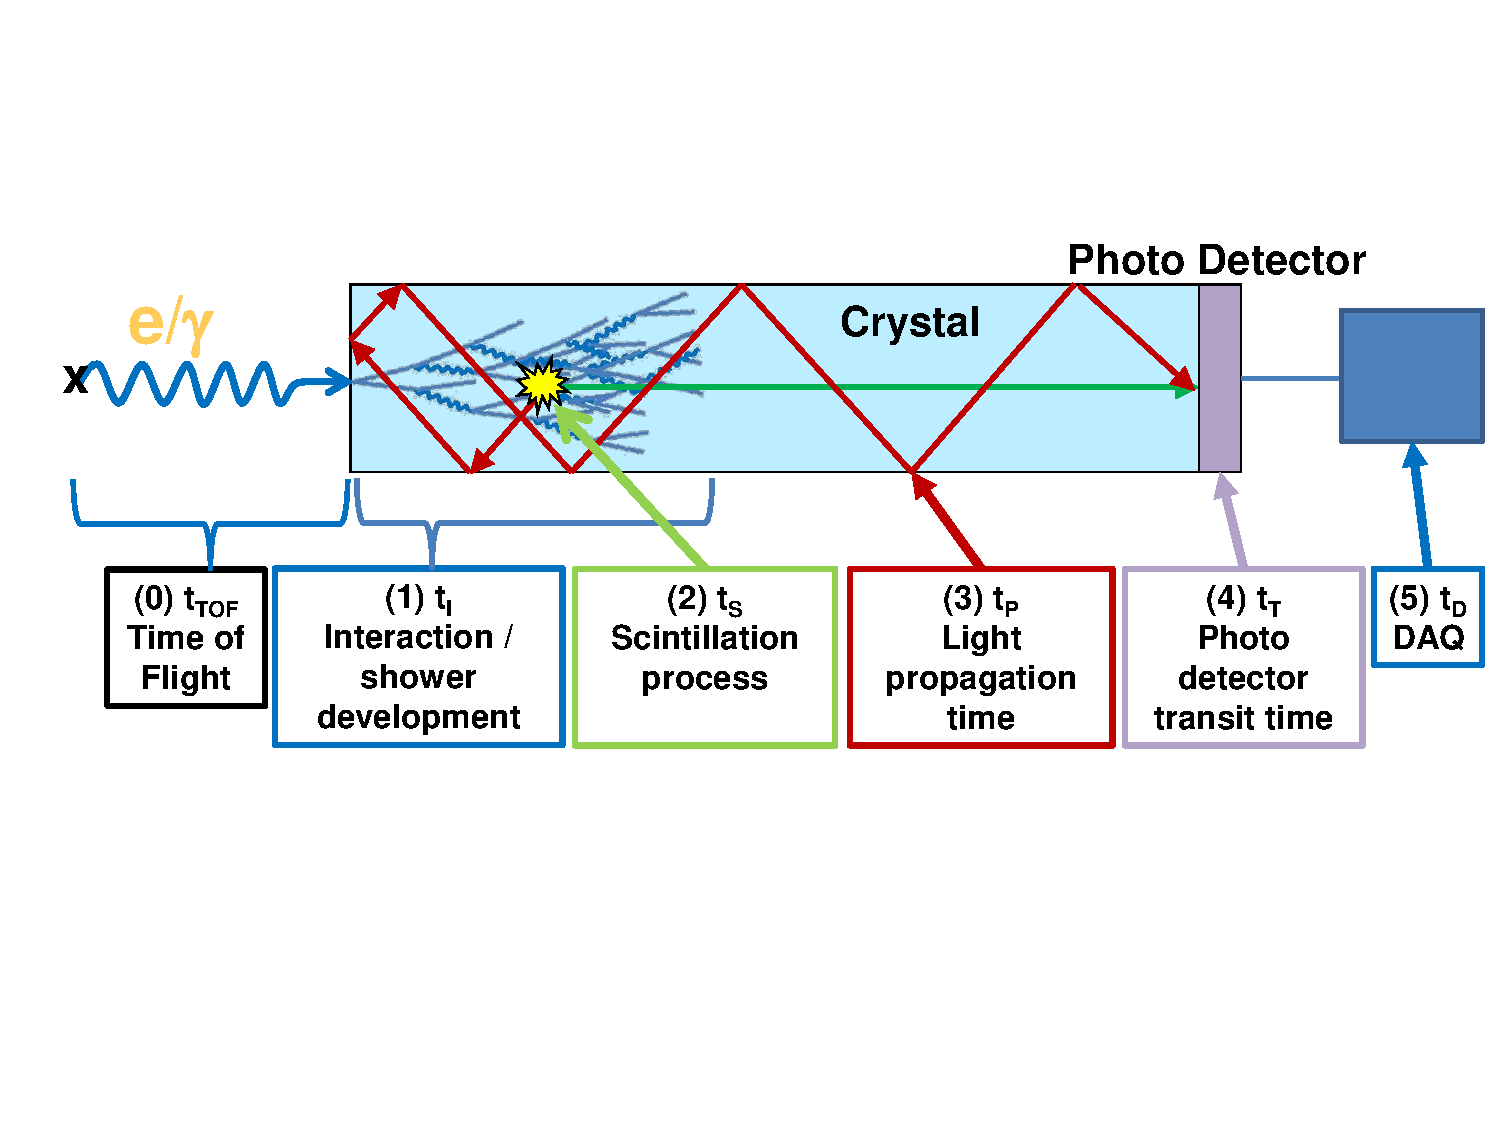
\includegraphics[width=0.85\textwidth]{figs/ScintillatorTiming_v4}
\caption{\small Timing measurement schematic breakdown using a monolithic, large scintillating crystal. 
The incident particle impinges on the crystal face from the left. The characteristic time intervals  are discussed 
in the text.}
\label{fig:ScintillatorTiming}
\end{figure}

Previous studies~\cite{MCPFastCaloNIMA}, measured the time resolution at different
absorber thickness for electron beams with energies varying from $12$ to
$32$~GeV, and showed that the time of arrival of the front of an electromagnetic
shower can be determined with a precision better than $20$~ps. The electronic
time resolution of the DAQ system was measured to be about $6$~ps. Using
the same techniques, we measure the time resolution of the MCP-PMT photodetectors 
used in the studies presented in this paper  to be between $11$~ps and $14$~ps, depending 
on the exact device.

To characterize the time resolution of an inorganic crystal scintillator calorimeter we
study the contributions due to fluctuations in the shower development, scintillation process, 
and light propagation to the photodetector.  We take advantage of the very large number of 
scintillation photons in a LYSO crystal which result in modest fluctuations associated with the 
creation and transit of each particular scintillation photon for a LYSO-based detector. 

 

\section{Experimental Setup}

A schematic diagram of a typical time of flight measurement setup is shown in 
Figure~\ref{fig:TypicalSchematicDiagram}. All measurements involve a fast photodetector,  
typically a micro-channel-plate photo-multiplier-tube 
(MCP-PMT), which  measures the reference ($t_{0}$) timestamp, and a photodetector further 
downstream that detects the signal associated with the electromagnetic shower and provides 
a simultaneous energy and time ($t_{1}$) measurement. 

\begin{figure}[H] \centering
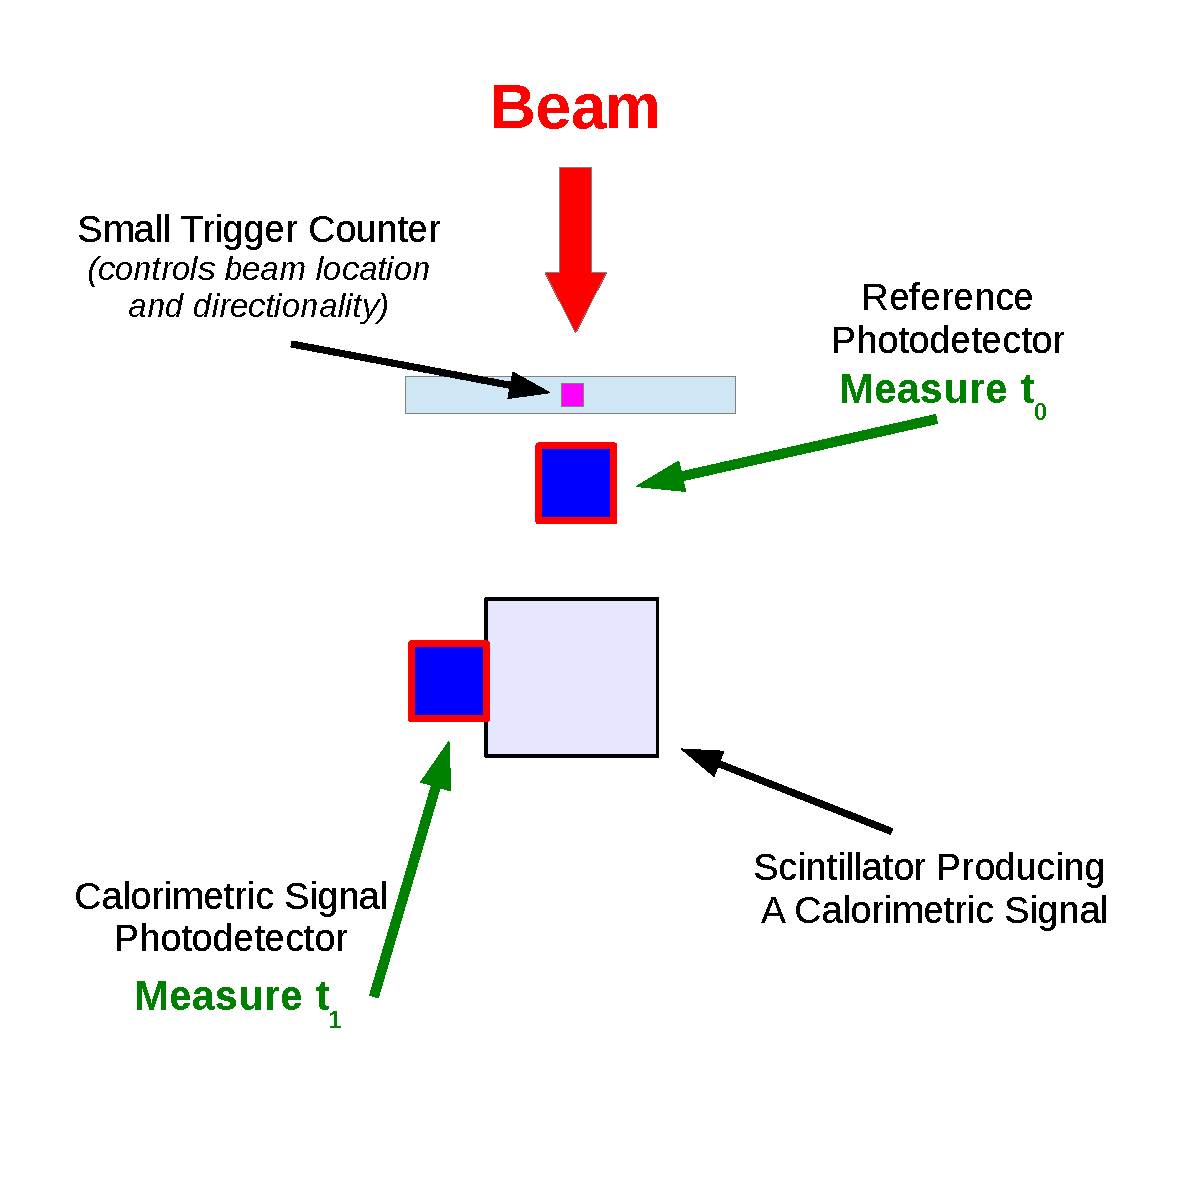
\includegraphics[width=0.45\textwidth]{figs/TypicalSchematicDiagram} 
\caption{\small The basic schematic diagram of the experimental setup for
a typical time of flight measurement is shown to illustrate the
basic detector elements. One photodetector is used as a time reference and the second 
measures energy and time simultaneously.} 
\label{fig:TypicalSchematicDiagram}
\end{figure}

In our study we used two types of MCP-PMT photodetectors, one produced by Hamamatsu 
(model R3809-52)~\cite{HamamatsuMCP3809}, and one produced by Photek (model
PMT240)~\cite{Photek240}. A DRS4  waveform digitizer V4 evaluation
board ~\cite{DRS4} was used as the primary DAQ system, connected to a laptop via
USB interface.  The DRS chip contains a switched capacitor array (SCA) with 1024 cells, 
capable of digitizing eight analog signals with high speed (5 GSPS) and high 
accuracy (11.5 bit SNR). All experimental beam studies were performed at the Fermilab Test
Beam Facility (FTBF), which provided proton beams from the Fermilab Main
Injector accelerator at $120$ GeV, and secondary electron beams of energies
ranging from $4$ to $32$~GeV. All detector elements were placed inside of a dark box
lined with copper foil, providing RF shielding. A $2$x$2$~$\mathrm{mm}^{2}$
scintillator was placed inside the box at the upstream extremity and used to
trigger the DAQ readout, providing a strict constraint on the
location and directionality of the beam particles used in the time of flight
studies. A differential Cherenkov counter (not shown in the schematic)  provided by the FTBF
facility and located upstream of our experimental hall,  was used for electron
identification. 

\section{Event Selection and Data Analysis}

Our primary target is to reconstruct the time of flight of beam particles between
different detector elements. Different time reconstruction algorithms are used
for different detector elements, and all involve the assignment of a timestamp
using specific features of each corresponding signal pulse. The signal pulse for
the reference time detector is very sharp and symmetric around its maximum
amplitude, as shown in Figure~\ref{fig:PulseShapes}. Hence for the reference
detector we determine the time position of the pulse peak by fit a Gaussian
function to the peak of the pulse, using three sampling points before the pulse
maximum and four sampling points after. The fitted mean parameter of the
Gaussian function is assigned as the timestamp $t_{0}$. The signal pulse for the
downstream time measurement is the result of scintillation light, and exhibits a
fast rising edge and a significantly slower decay. Therefore, we assign the
timestamp $t_{1}$ using a constant fraction of the rising edge. A linear
function is fit to the sampling points between $10\%$ and $60\%$ of the pulse
maximum and the timestamp is assigned as the time at which the fitted linear
function rises to $20\%$ of the pulse maximum. Examples of fits performed to
assign a time stamp from each pulse are shown in Figure~\ref{fig:PulseFits}. The
impact from the choice of the functional forms is studied by using a set of
alternative functions in the fits, and choosing the one that results in the best
time resolution. Among the functions that we tested, the difference between the
best and worst performing functions was about 8~psec.

\begin{figure}[h] \centering
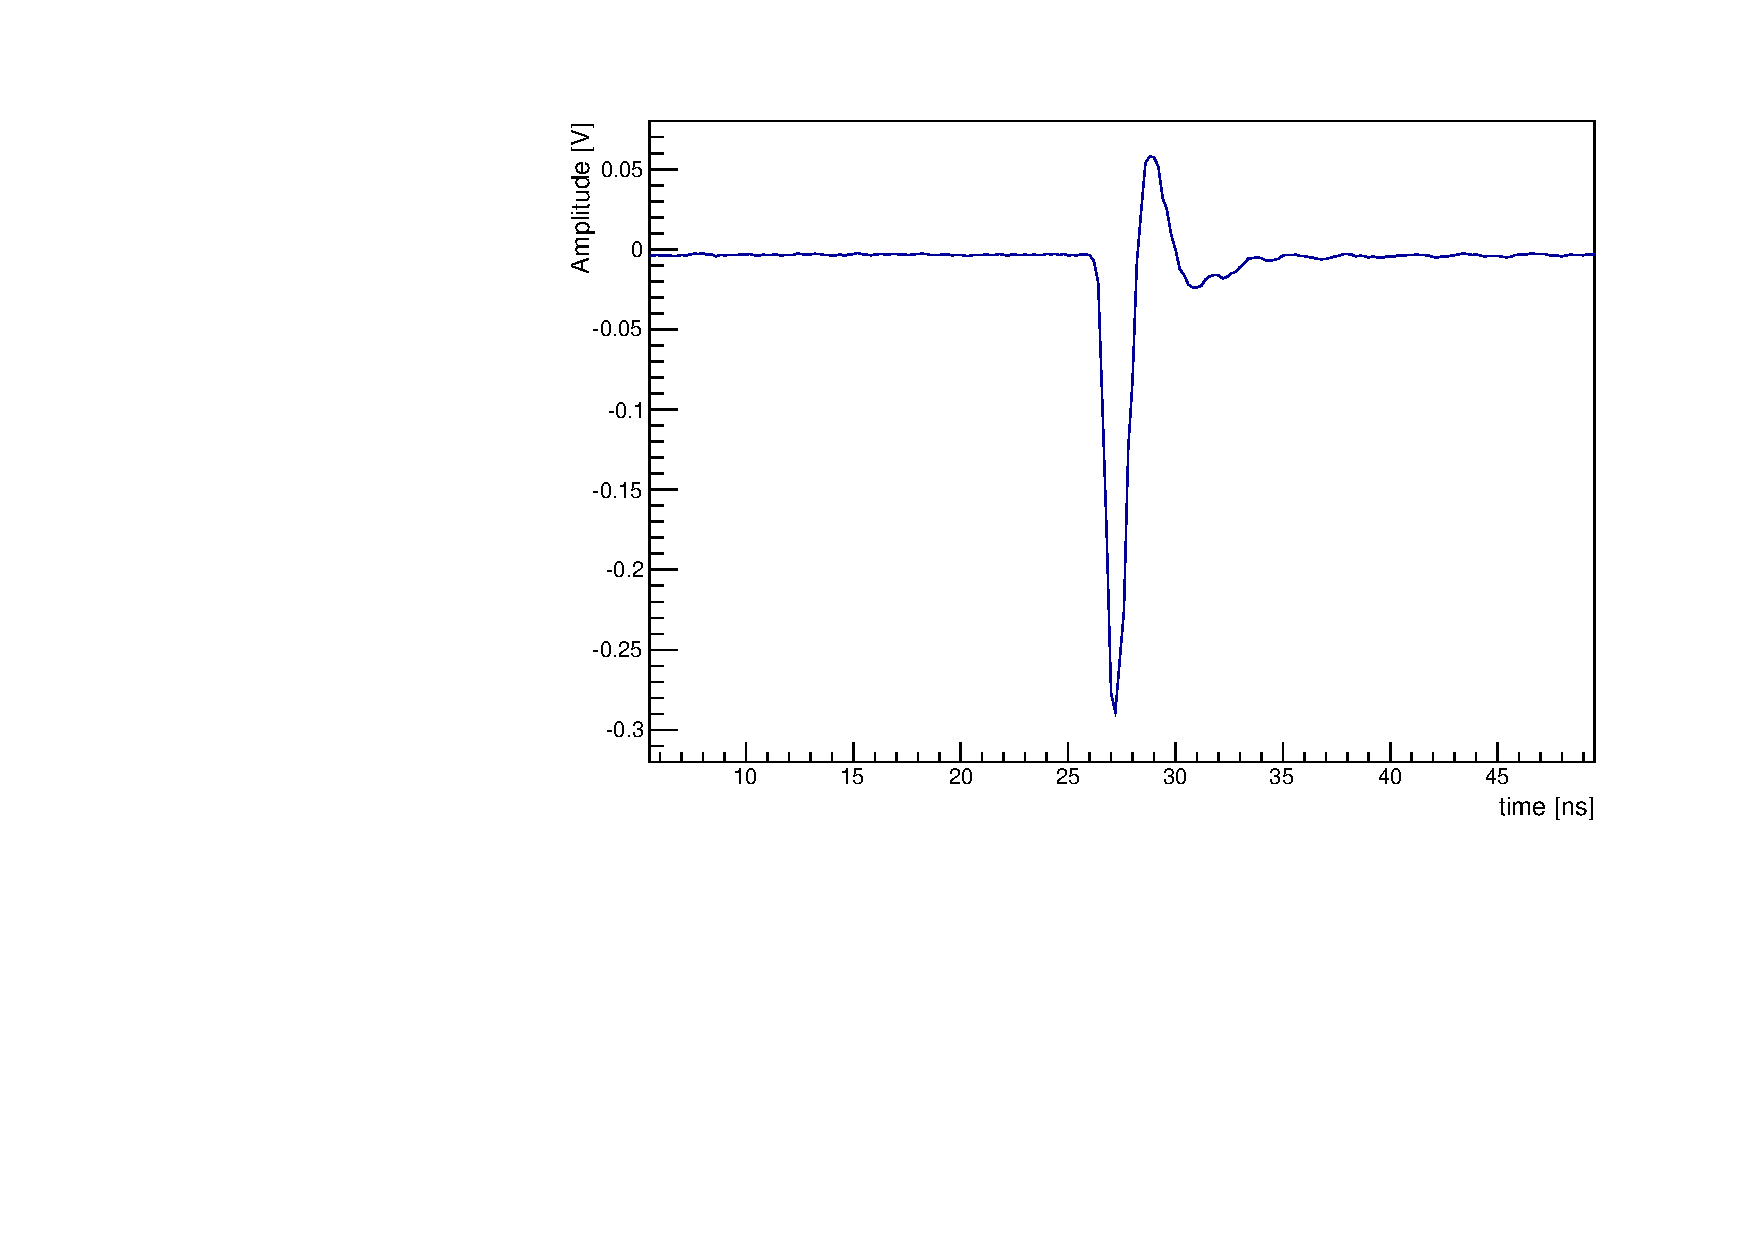
\includegraphics[width=0.45\textwidth]{figs/RefPulse} 
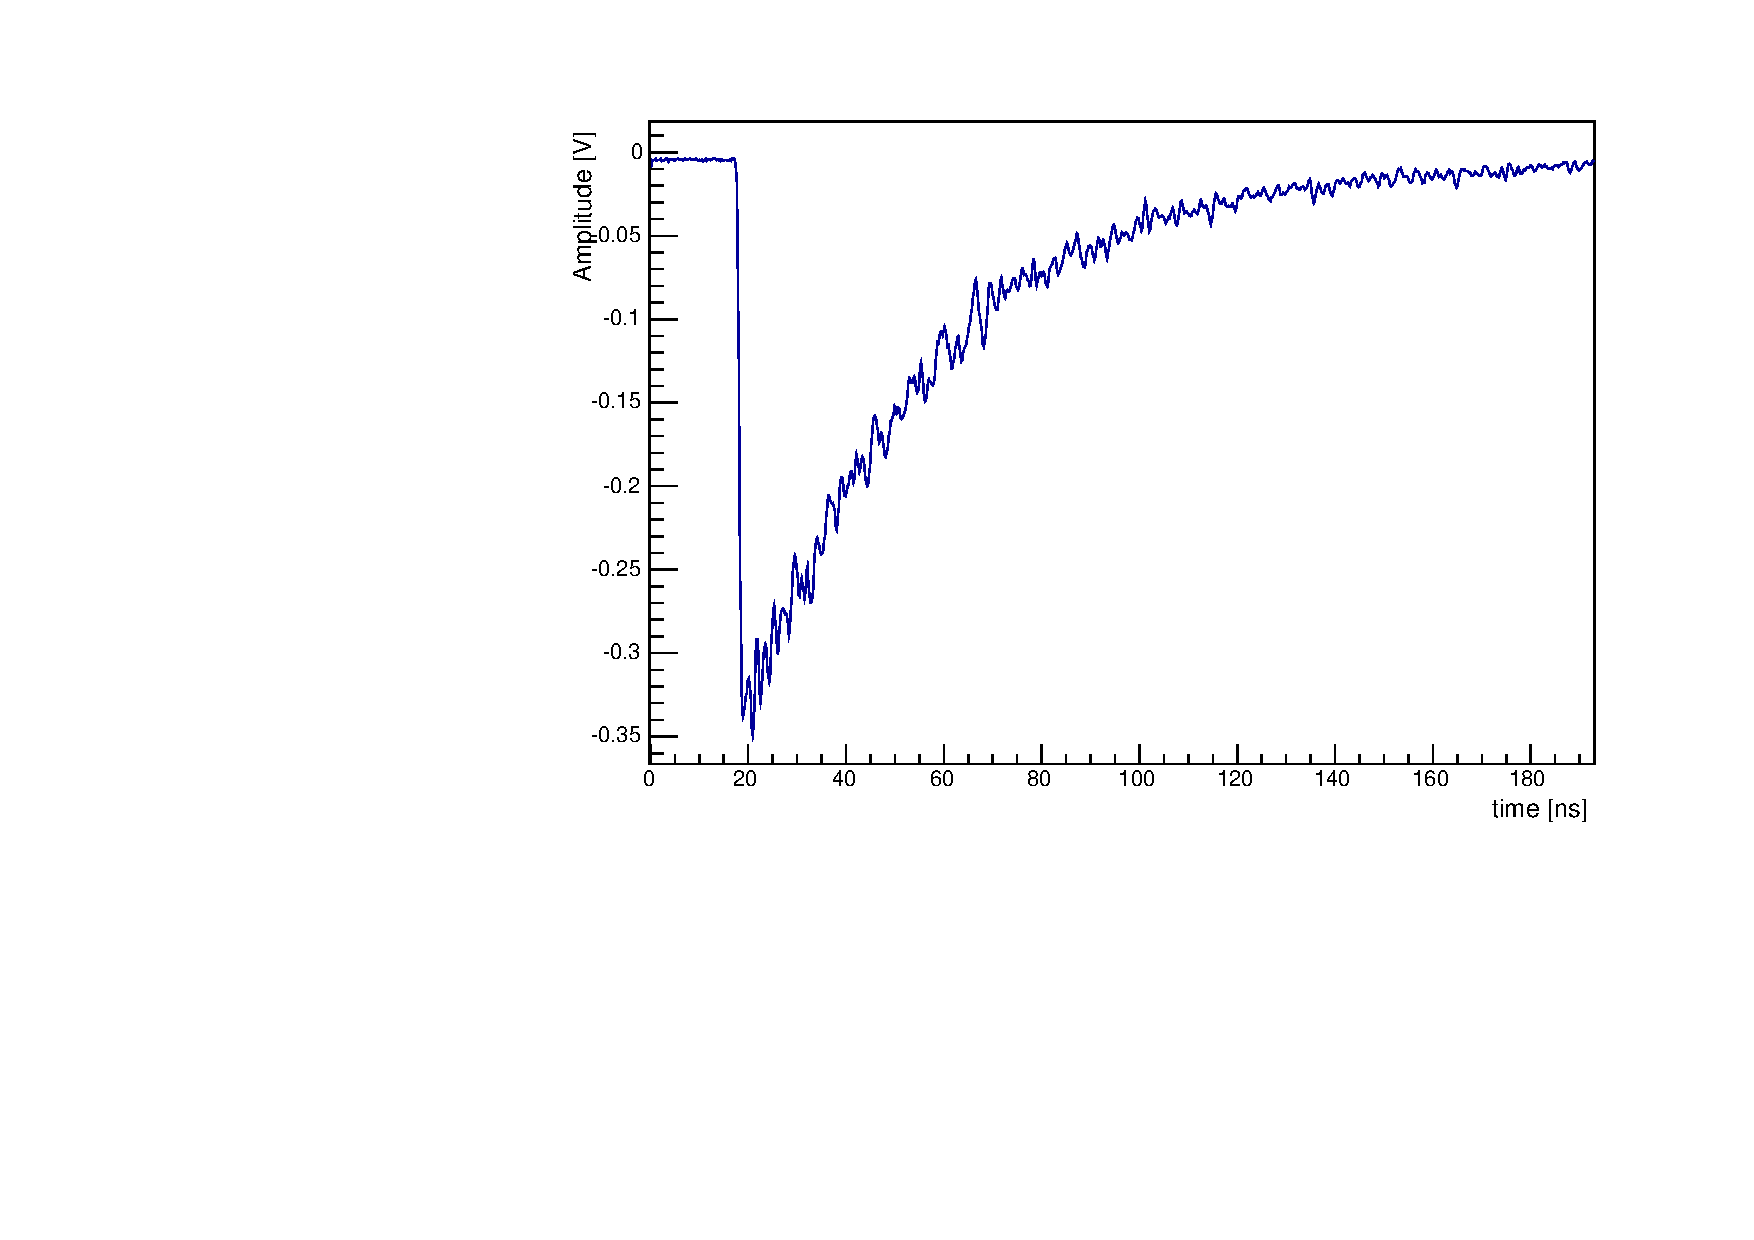
\includegraphics[width=0.45\textwidth]{figs/run064_event506} 
\caption{\small Sample pulses as digitized by the DRS4 board. 
On the left a pulse is shown from the reference Hamamatsu R3809 MCP-PMT, 
and on the right is a pulse from the Hamamatsu R3809 MCP-PMT
optically coupled to a (1.7~cm)$^{3}$ LYSO crystal cube
recorded using  8 GeV electron beam.} 
\label{fig:PulseShapes}
\end{figure}

Event selection and pulse cleaning procedures are used to eliminate abnormal
pulses in the readout, as described in~\cite{MCPFastCaloNIMA}. Large signals
above 500 mV are rejected because they saturate the DRS4 inputs. Only pulses
with amplitude larger than 20 mV are used for time of flight measurements, in
order to reduce the impact of noise from the DRS waveform digitizer DAQ system.
Events containing more than one pulse within the $200$~ns readout window are not
used. Attenuators were used to extend the dynamic range of the DRS4
waveform digitizer in cases when a large fraction of signal pulses are saturated.

\begin{figure}[h] \centering
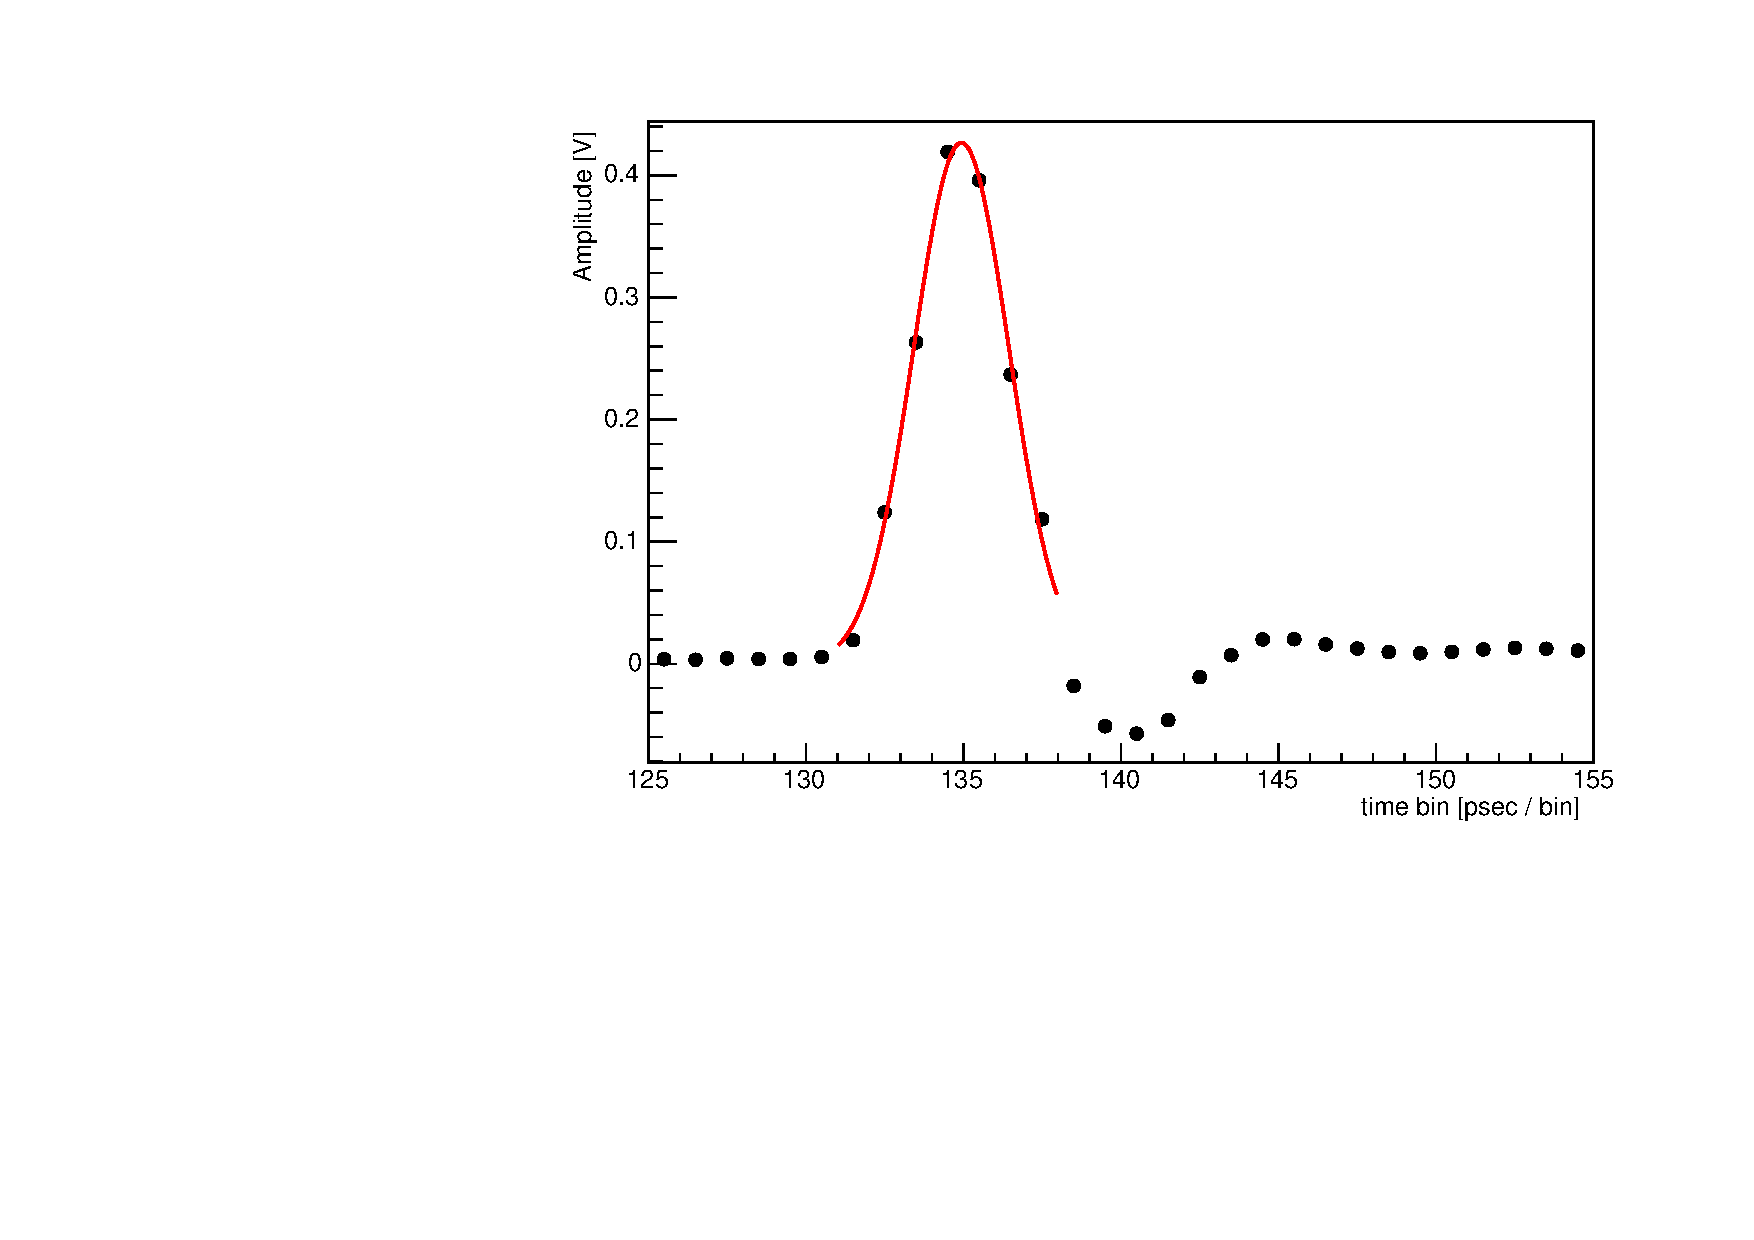
\includegraphics[width=0.45\textwidth]{figs/Reference_Pulse_GausFit_057_ev322.pdf} 
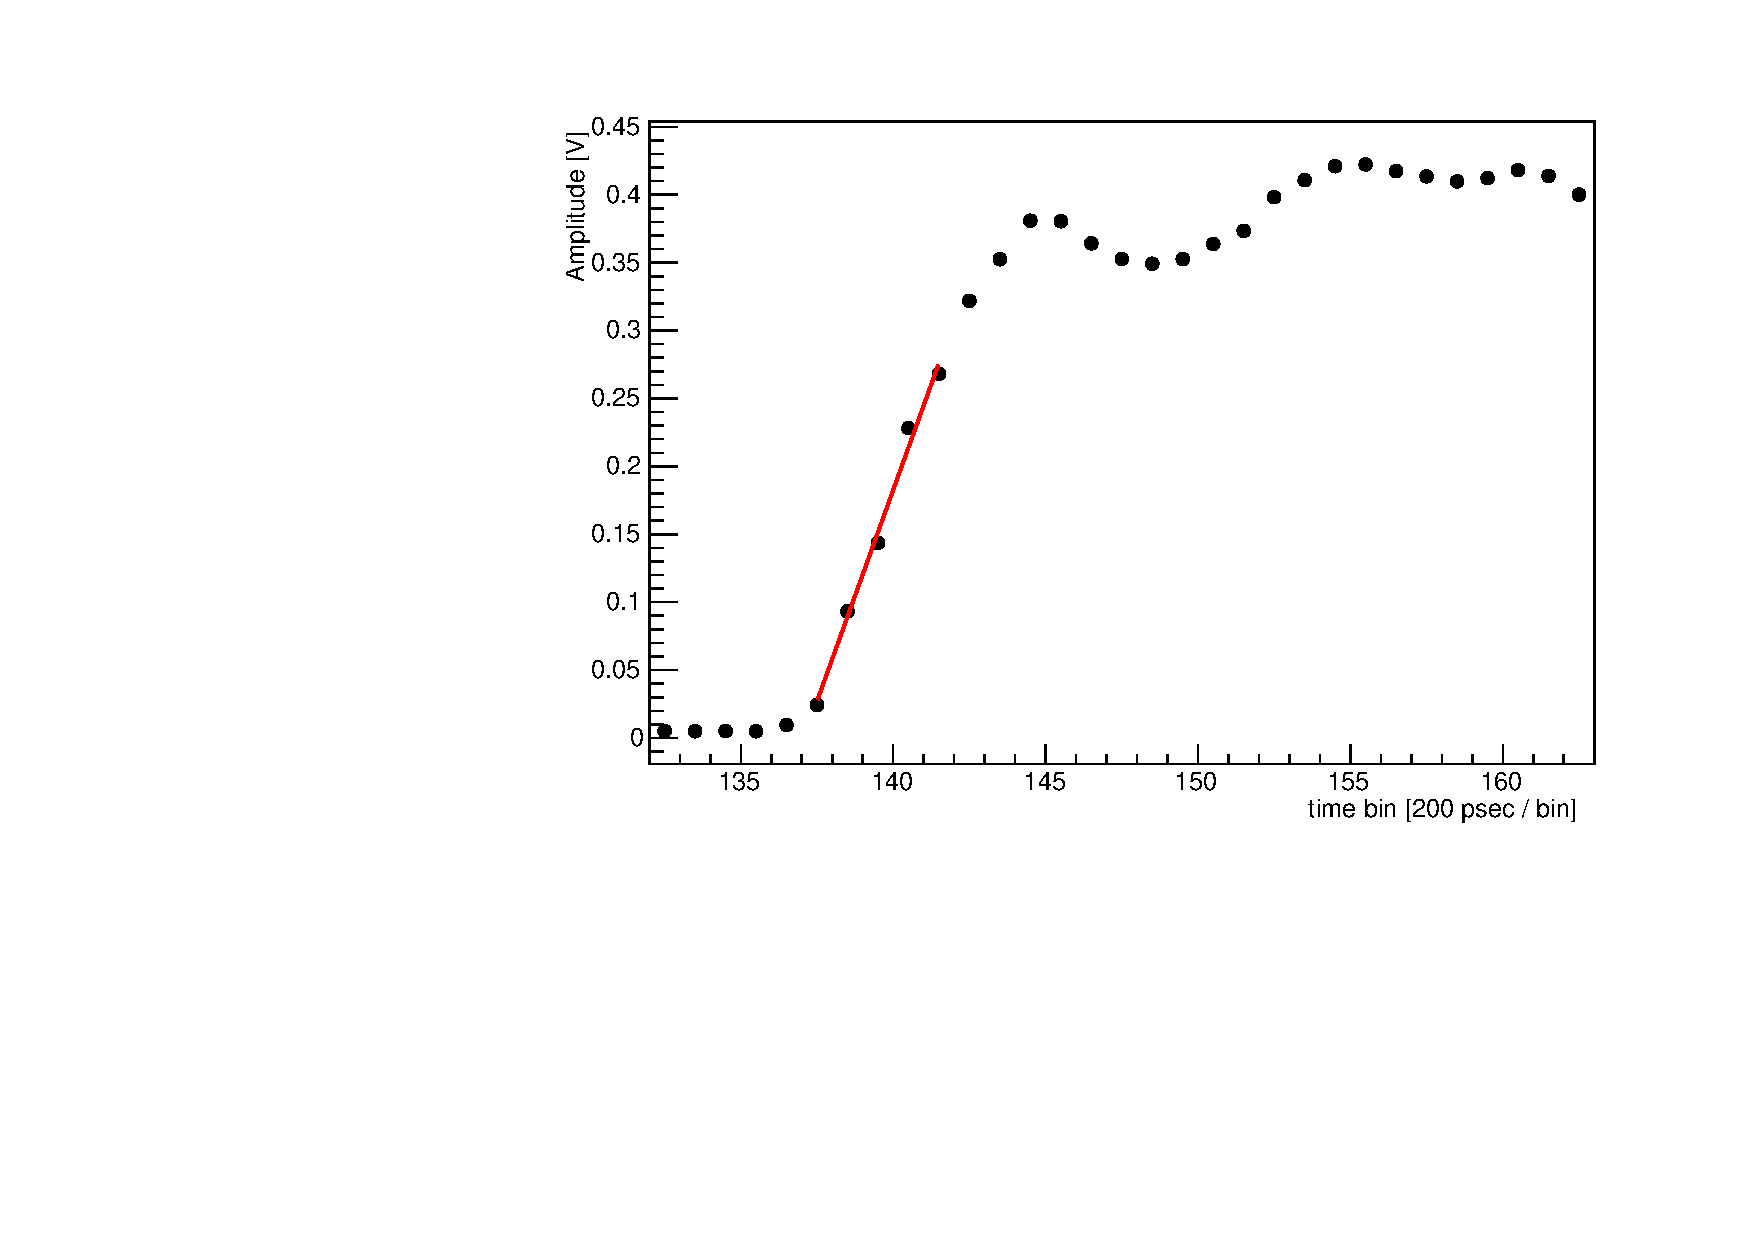
\includegraphics[width=0.45\textwidth]{figs/LYSOCube_Pulse_RisingEdgeFit_057_ev313.pdf} 
\caption{\small Sample fits used to assign timestamps to digitized MCP-PMT pulses. 
On the left is a pulse from the reference Hamamatsu R3809 MCP-PMT, and
on the right is a pulse from the Hamamatsu R3809 MCP-PMT
optically coupled to a (1.7~cm)$^{3}$  LYSO crystal
recorded during an 8 GeV electron run.}
\label{fig:PulseFits}
\end{figure}


\section{Timing in LYSO-based Calorimeters}
The timing measurement in 
LYSO-based calorimeters is driven by three main factors  -- other  than the intrinsic transit 
time of the photodector itself and the DAQ electronics : a) the shower profile fluctuations,  
b) the scintillation time, and c) the light propagation time. Stochastic processes during the
development of an electromagnetic shower affect the time of observed signals, as
both the transverse size and the depth of the shower can fluctuate event-by-event. 
Random processes in the scintillation mechanism and the randomization of
the optical paths for the scintillation light affect both the speed of the
signal formation and the time jitter. We study these effects using two
independent experimental setups. 

For a  homogeneous crystal calorimeter we are interested in the characterization and 
optimization of the light propagation time, i.e. the time the scintillation light travels
down the length of the crystal. Our setup uses a small LYSO cube with linear dimensions 
of $17\mathrm{mm}$ as the active scintillation element. The size of this element reduces 
the effect of the light propagation time and jitter. The LYSO cube is placed behind about 
$4.5~X_0$ radiation lengths of lead. Using this LYSO-based sampling calorimeter, we
measure the time resolution of electrons.

We also study a shashlik calorimeter composed of alternating layers of
tungsten and LYSO, in which scintillation light is extracted through wavelength
shifting (WLS) fibers. In this setup, the light propagation time through the fiber is the
dominant factor of the timing measurement. We study as a baseline an alternate version of this
calorimeter where the light is extracted through direct optical coupling of  the 
photodetectors at the edges of a few LYSO layers to minimize  the light propagation time.


\subsection{Timing Studies of the LYSO-based Sampling Calorimeter}

We study the combined impact of the shower profile fluctuations, the
scintillation mechanism in LYSO, and the light propagation time resolution
using a sampling calorimeter with a (1.7~cm)$^{3}$ LYSO cube as active
element. The LYSO crystal is wrapped in Tyvek and attached to the Hamamatsu
R3809 MCP-PMT (HAMB) with optical coupling~\cite{grease}.   A second Hamamatsu 
MCP-PMT  photodetector (HAMA)  is placed upstream of the calorimeter and is used 
to measure the reference time. A schematic diagram and a photograph of the experimental setup
are shown in Figure~\ref{fig:LYSOSamplingCaloSetup}. 

\begin{figure}[h] \centering
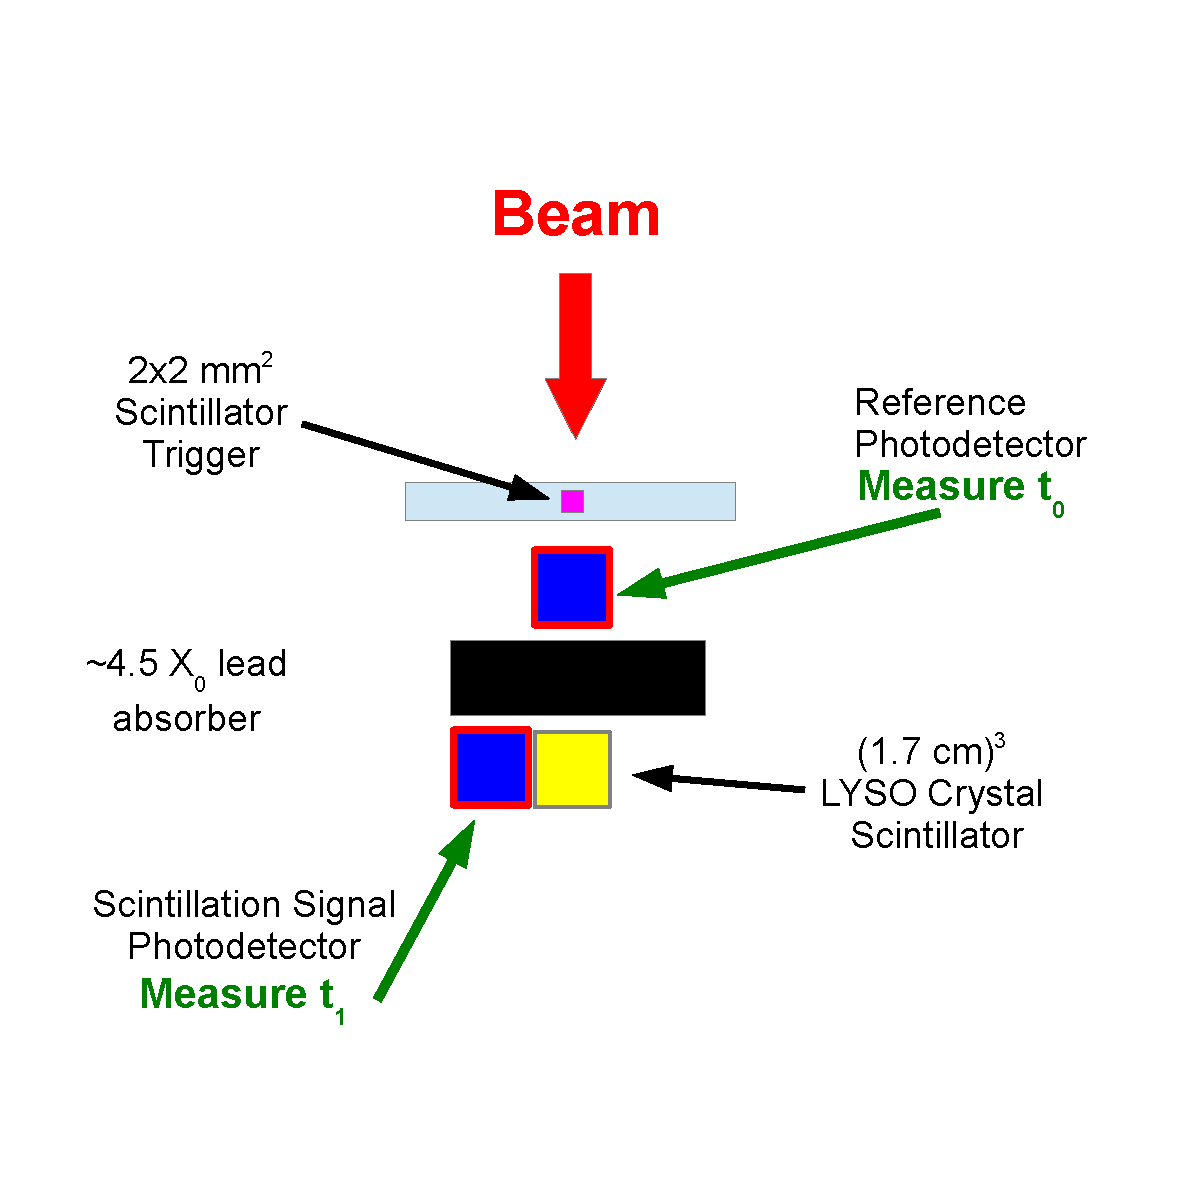
\includegraphics[width=0.45\textwidth]{figs/LYSOSamplingCaloSetupSchematic} 
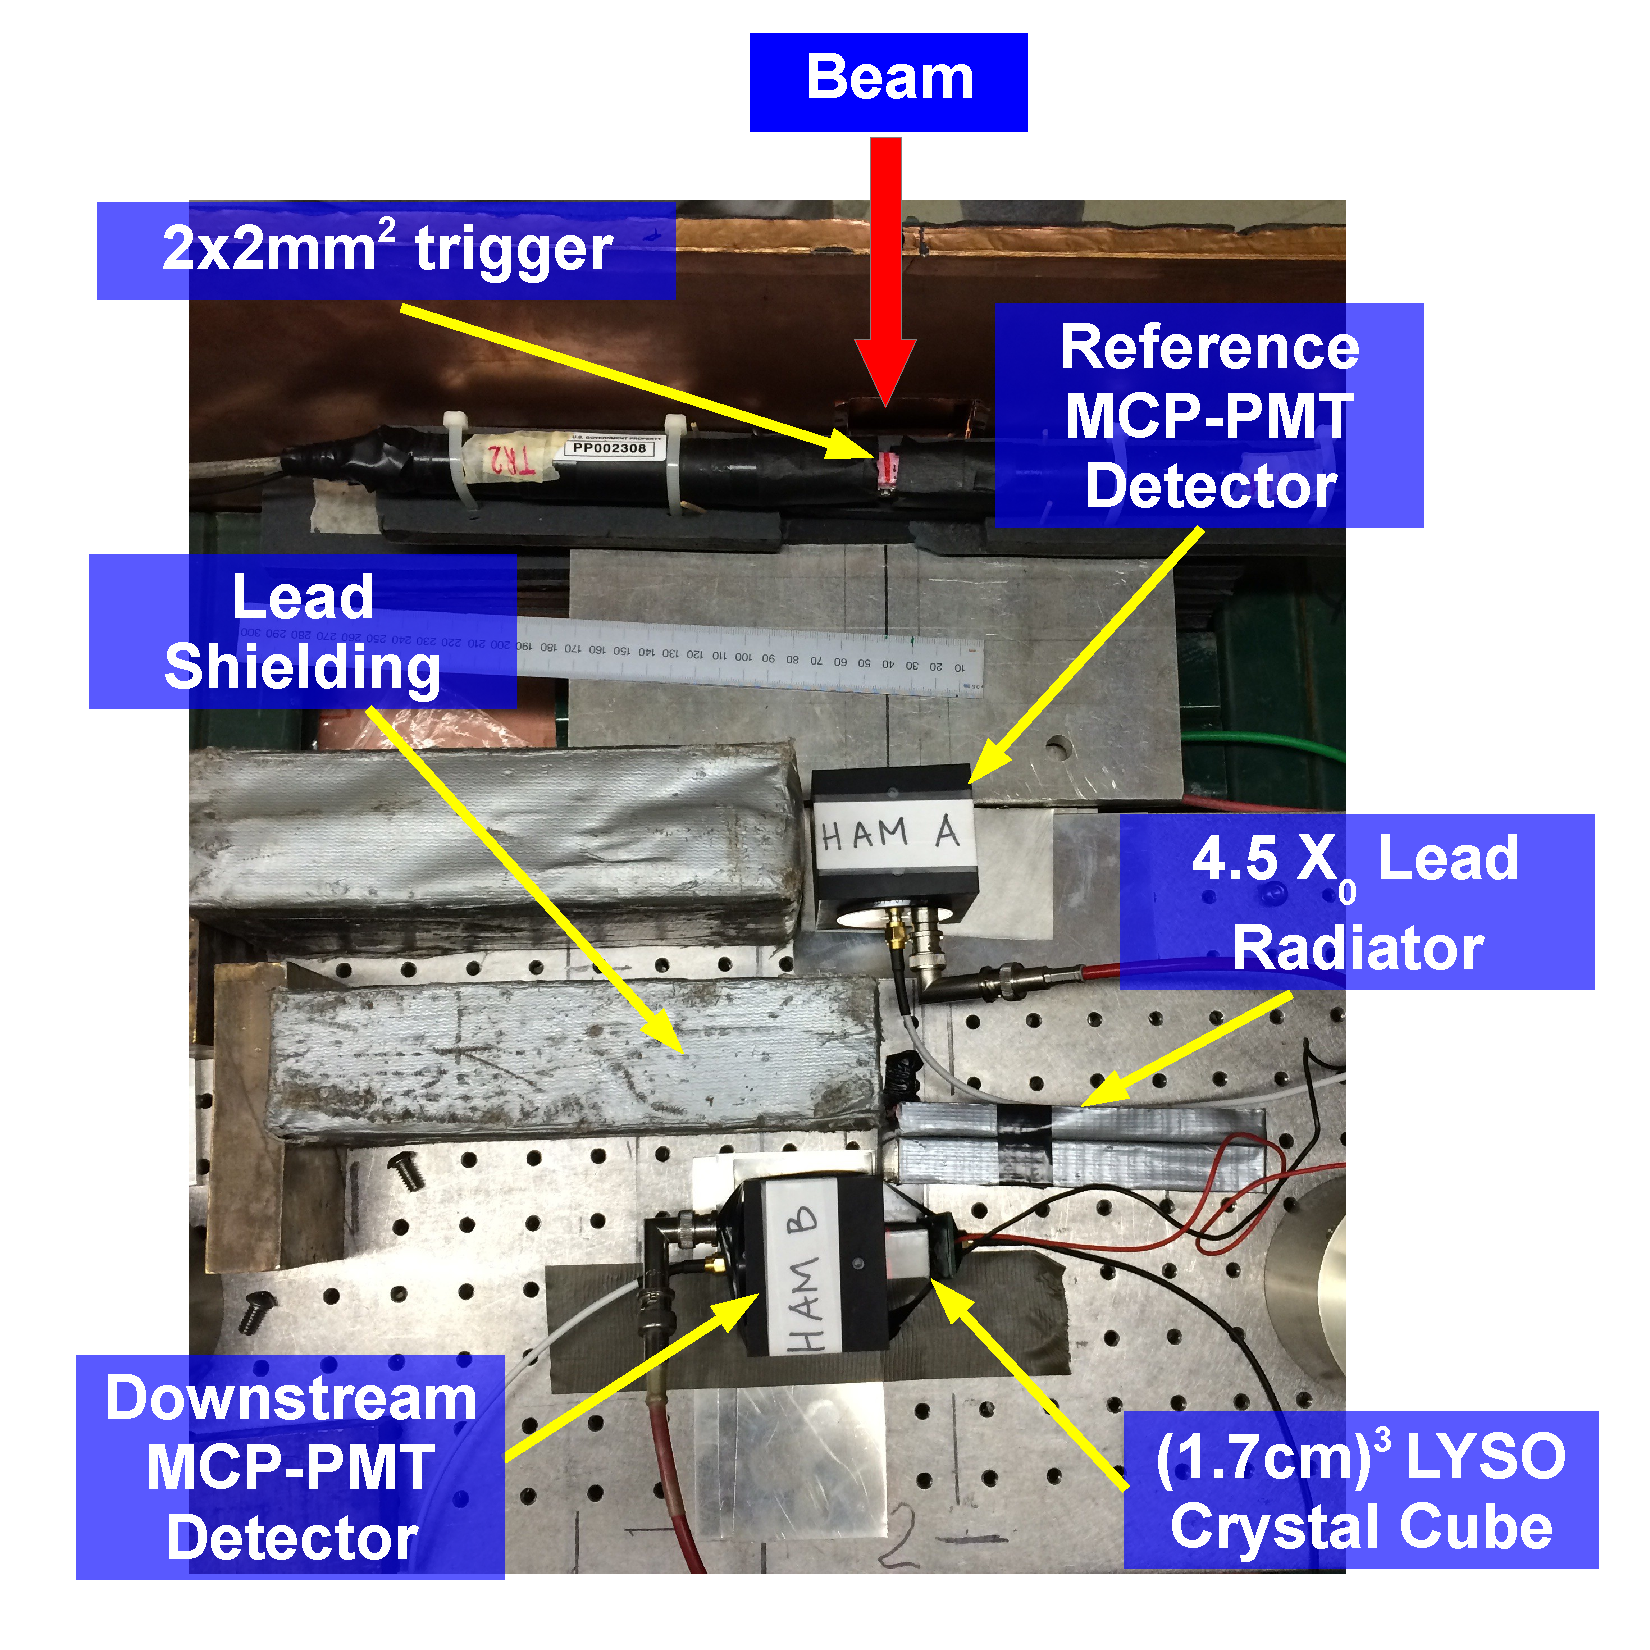
\includegraphics[width=0.45\textwidth]{figs/LYSOSamplingCaloSetupPhoto} 
\caption{ \small A schematic diagram of the experimental setup for the
time of flight measurement using the LYSO sampling calorimeter is shown
on the left, along with a picture of the experimental setup shown on the right. } 
\label{fig:LYSOSamplingCaloSetup}
\end{figure}

To ensure that the electron beam is constrained to within a $2\times 2$~mm$^2$ region, 
a plastic scintillator placed upstream and approximately $2$~mm by $2$~mm in cross sectional 
area is used to trigger the DAQ readout on the DRS  digitizer. Electron events are identified 
by requiring a signal with amplitude larger than $10$~mV in a Cherenkov counter located 
upstream. Large lead bricks are placed upstream of the Hamamatsu R3809 MCP-PMT (HAMB),
out of the path of the beam. These shield the photodetector from stray particles
produced in events where an electromagnetic shower occurs upstream of the lead
radiator. Such stray shower particles yield very fast signals which can
significantly contaminate the scintillation signal. Using the same experimental
setup without the LYSO active element in place, we find that stray shower type
events yield less than $10\%$ contamination and give a negligible effect on the
scintillation signal. 

%The same calorimeter setup with the Photek 240 MCP-PMT in
%place of the Hamamatsu R3809 MCP-PMT, which has an active area about $10$ times
%larger, is found to yield more than $80\%$ contamination and thus does not allow
%a proper measurement of the scintillation signal.

The thickness of the LYSO active element is relatively small and captures only a fraction 
of the total energy of the electron, but yields a reasonable energy measurement
as it is close to the shower maximum.

The time of flight measurement is performed using the LYSO sampling calorimeter
for electron beams with energies varying from $4$~GeV to $32$~GeV. The corresponding 
measured time of flight distributions are shown in Figure~\ref{fig:LYSOCubeTOF}.
We achieve the best time resolution of $34$~ps for electrons
with beam energy of $32$~GeV.

\begin{figure}[H] \centering
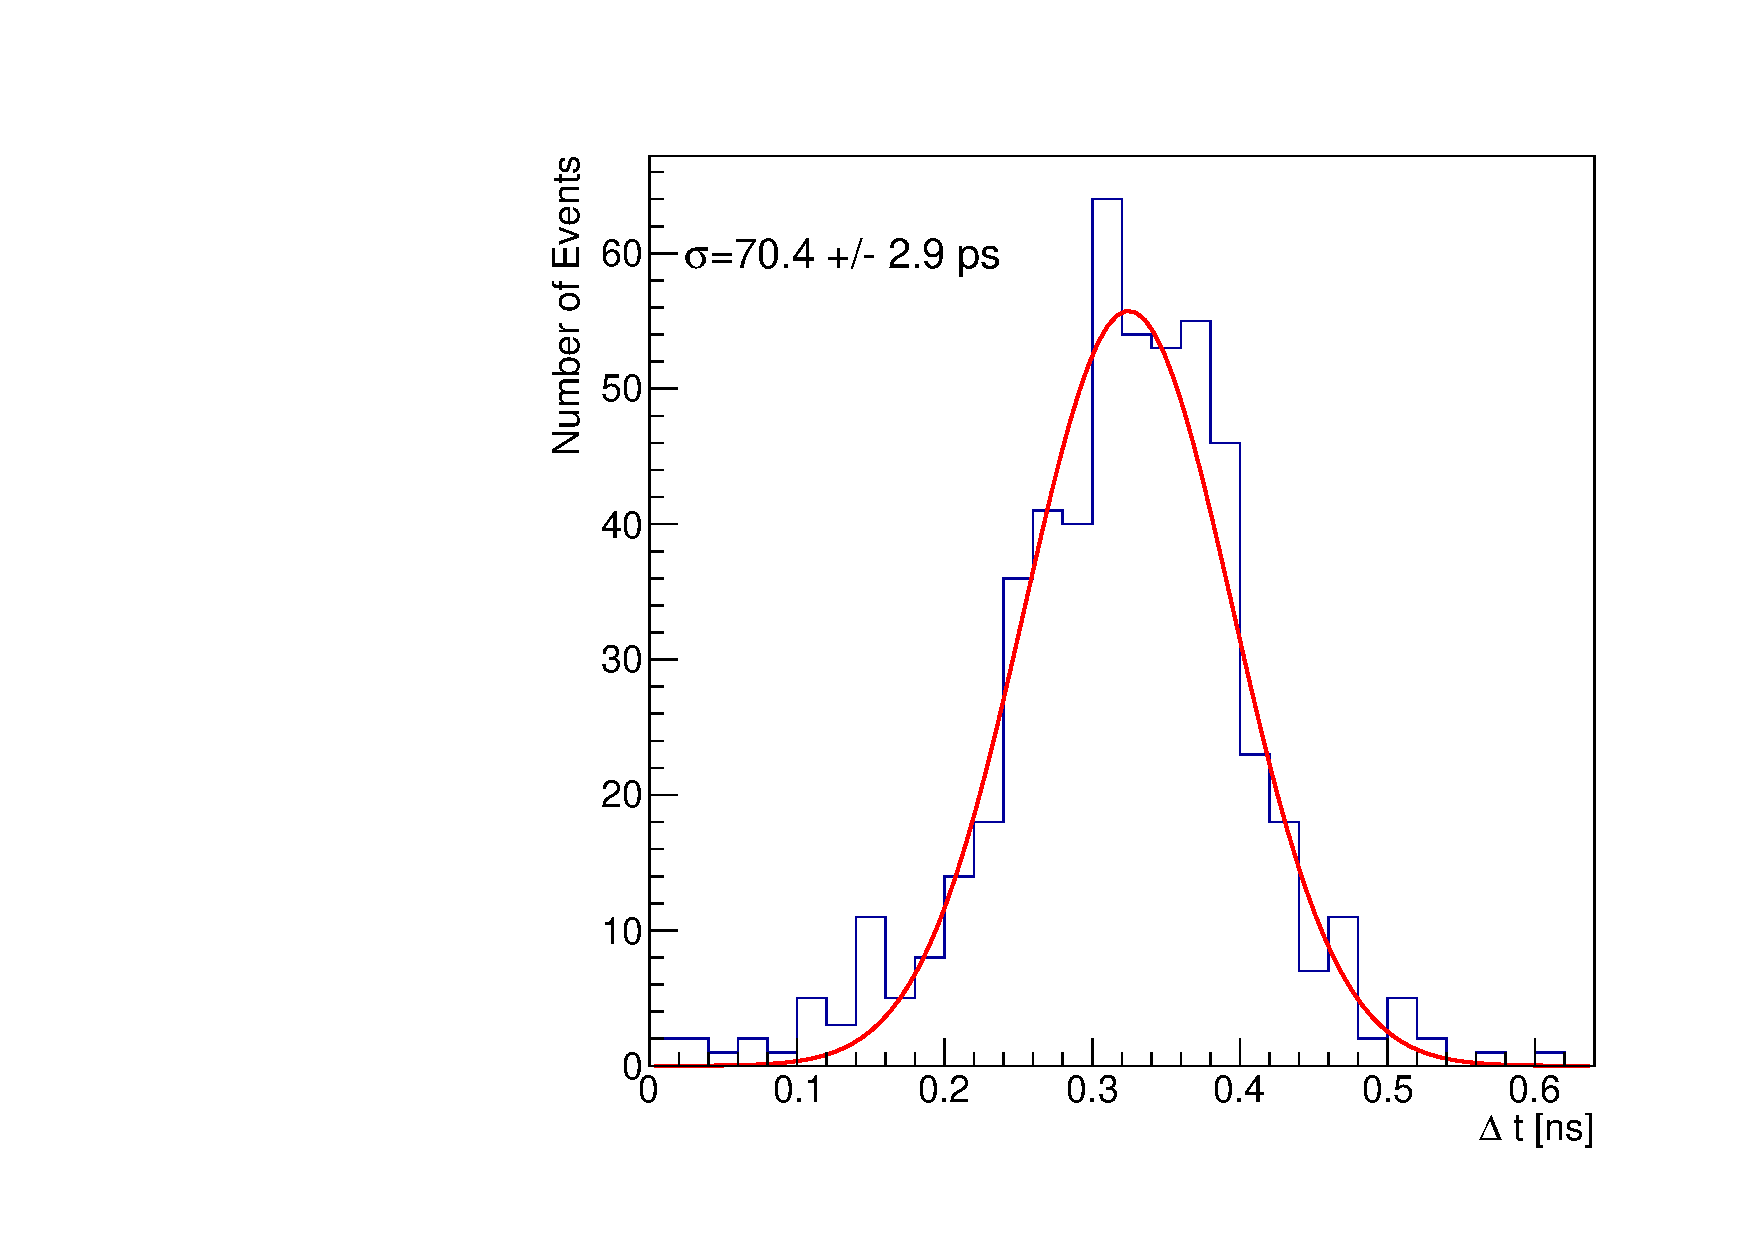
\includegraphics[width=0.23\textwidth]{figs/TOF_Electron_LYSOCube_4GeV} 
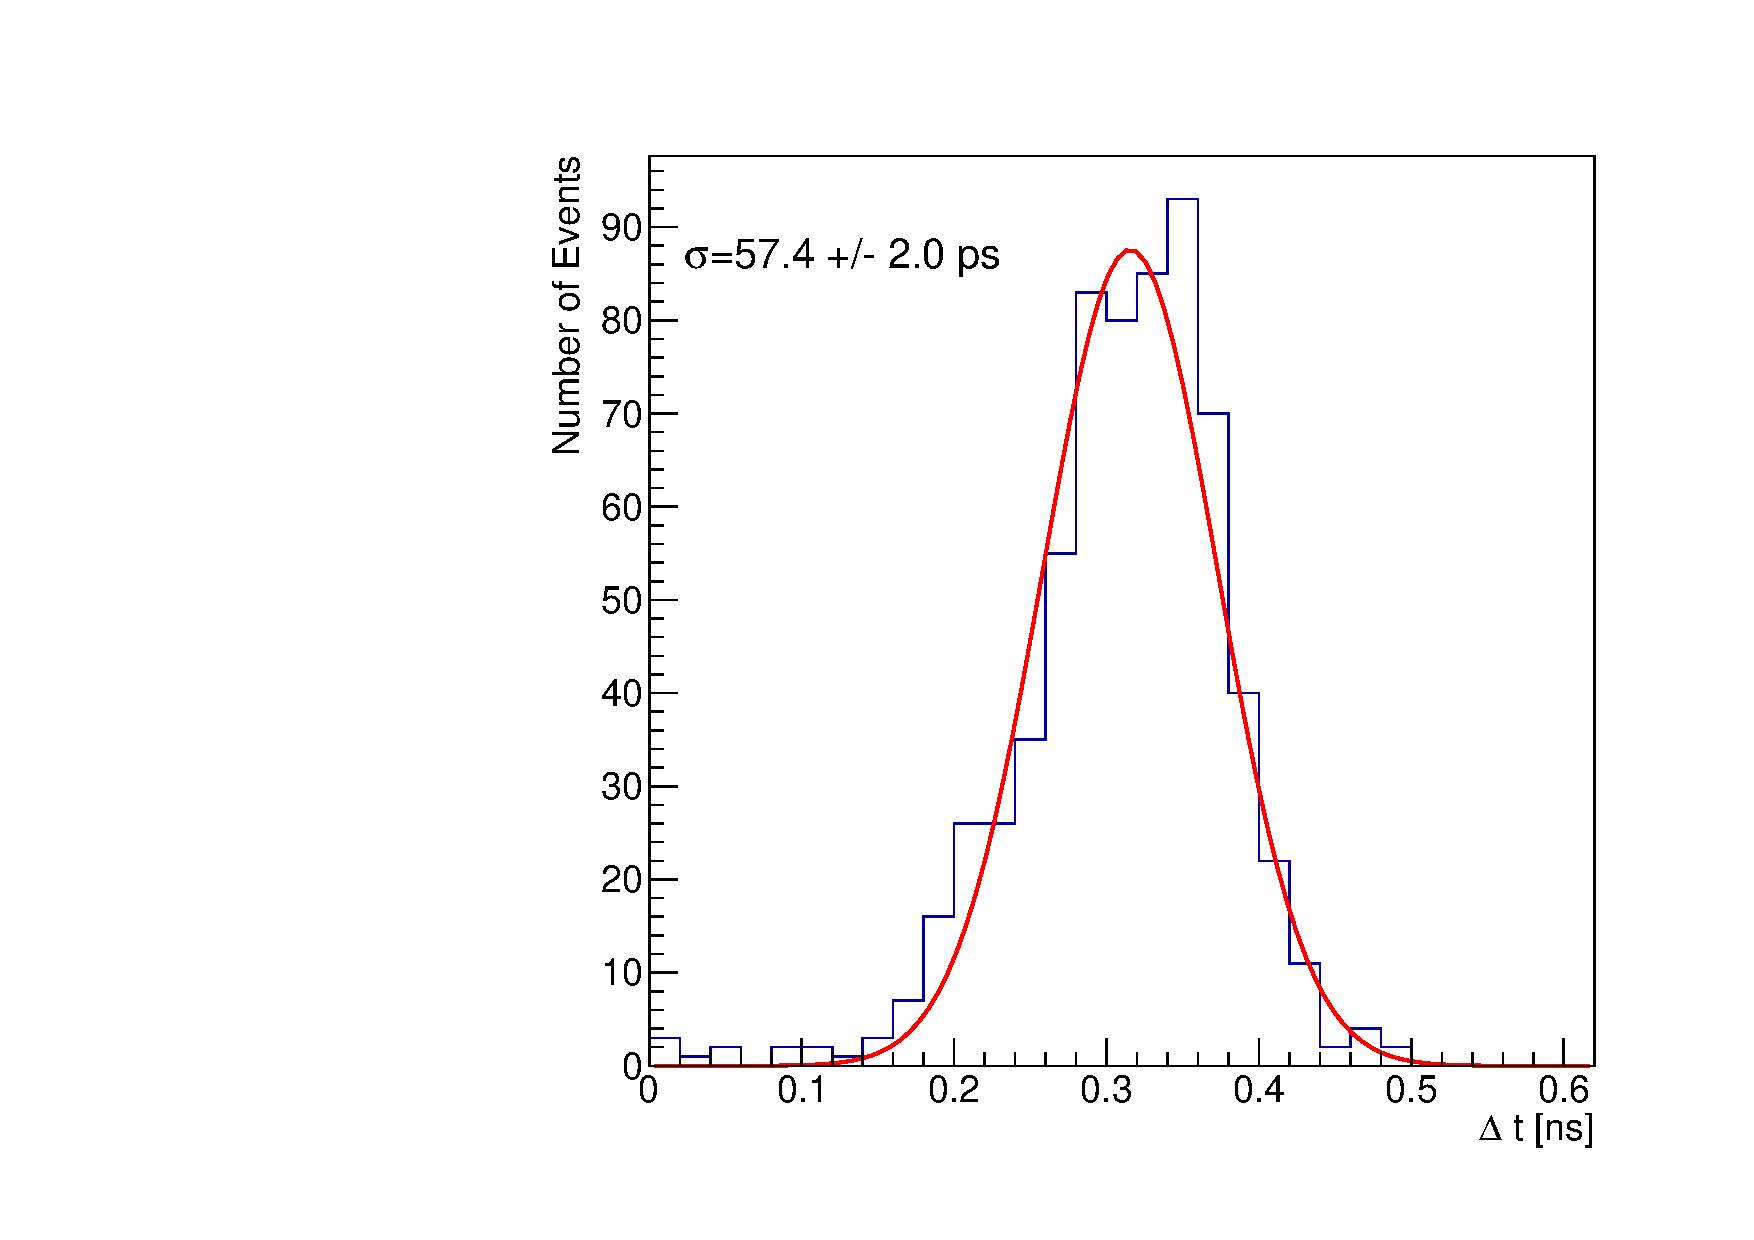
\includegraphics[width=0.23\textwidth]{figs/TOF_Electron_LYSOCube_8GeV} 
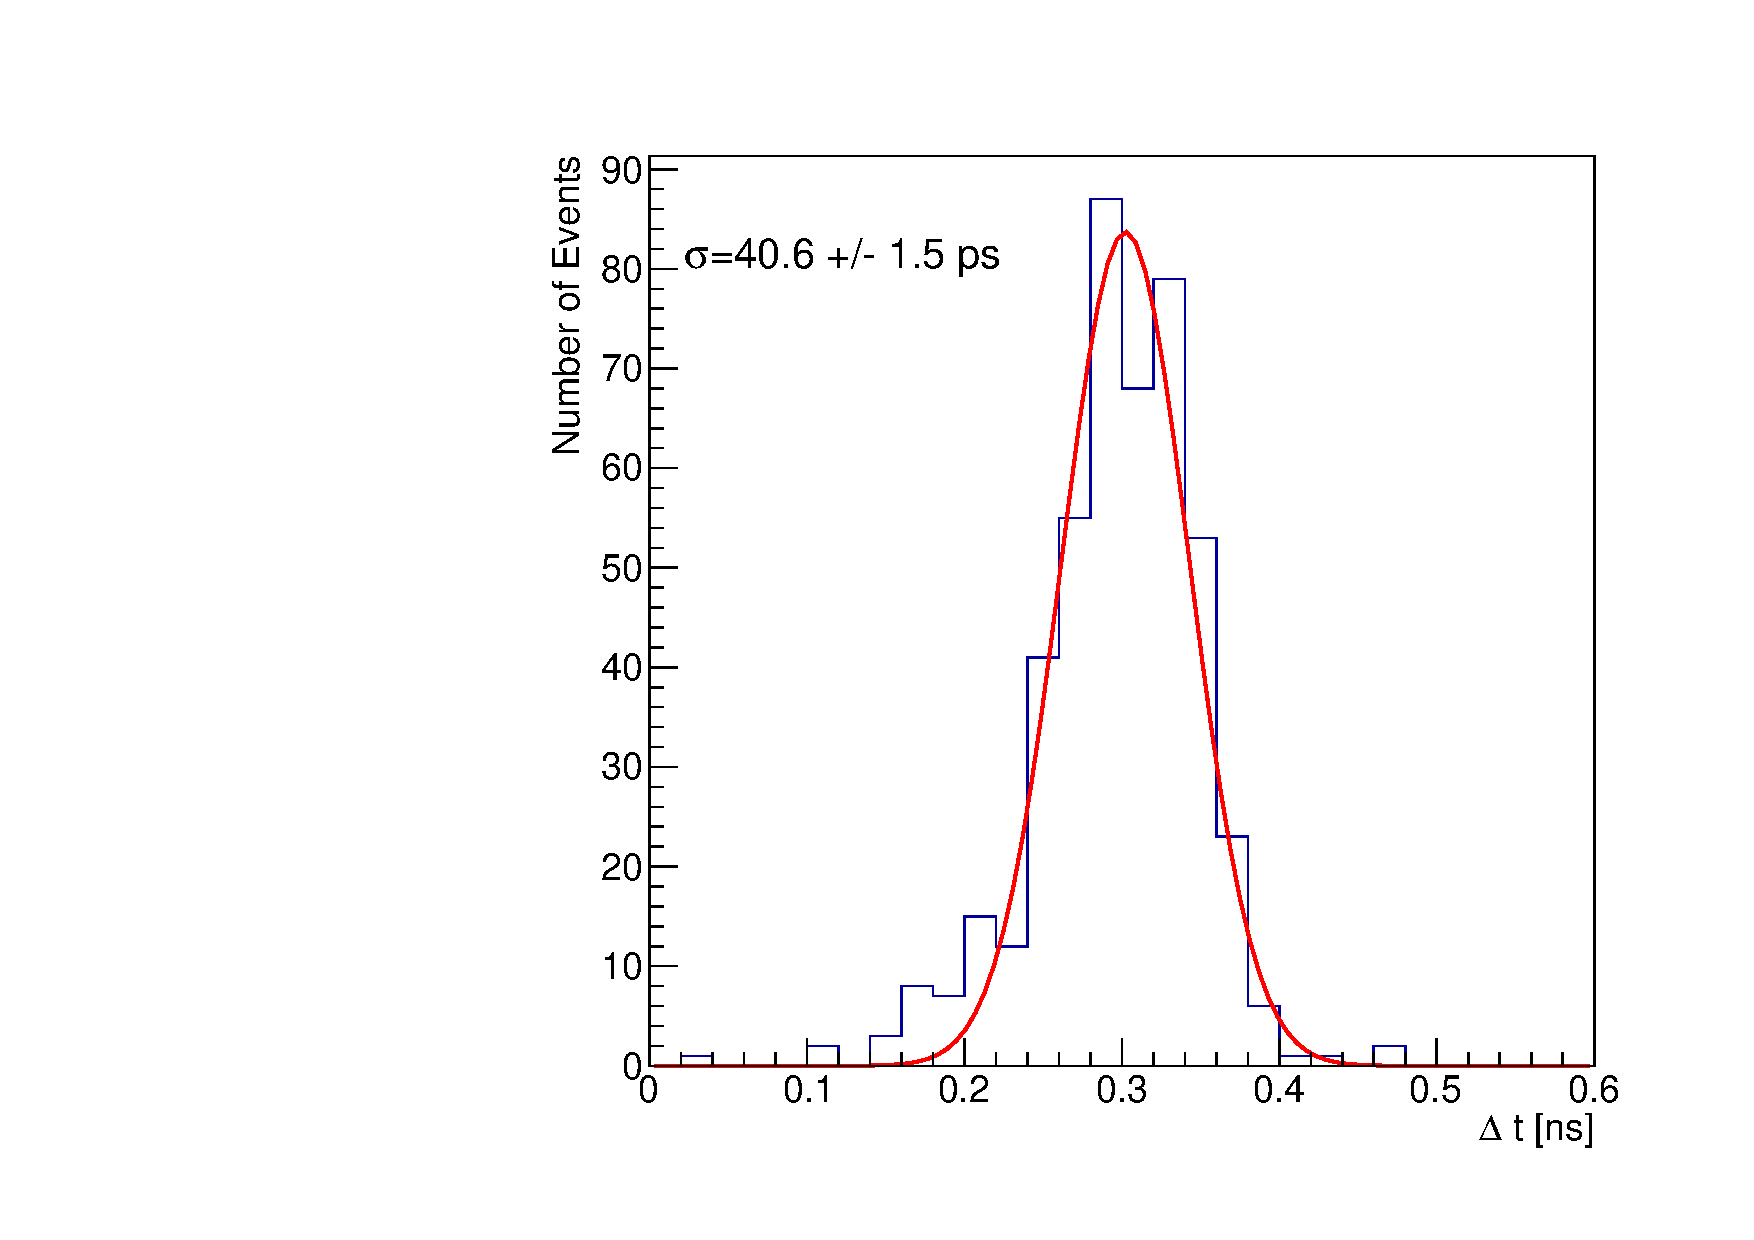
\includegraphics[width=0.23\textwidth]{figs/TOF_Electron_LYSOCube_16GeV} 
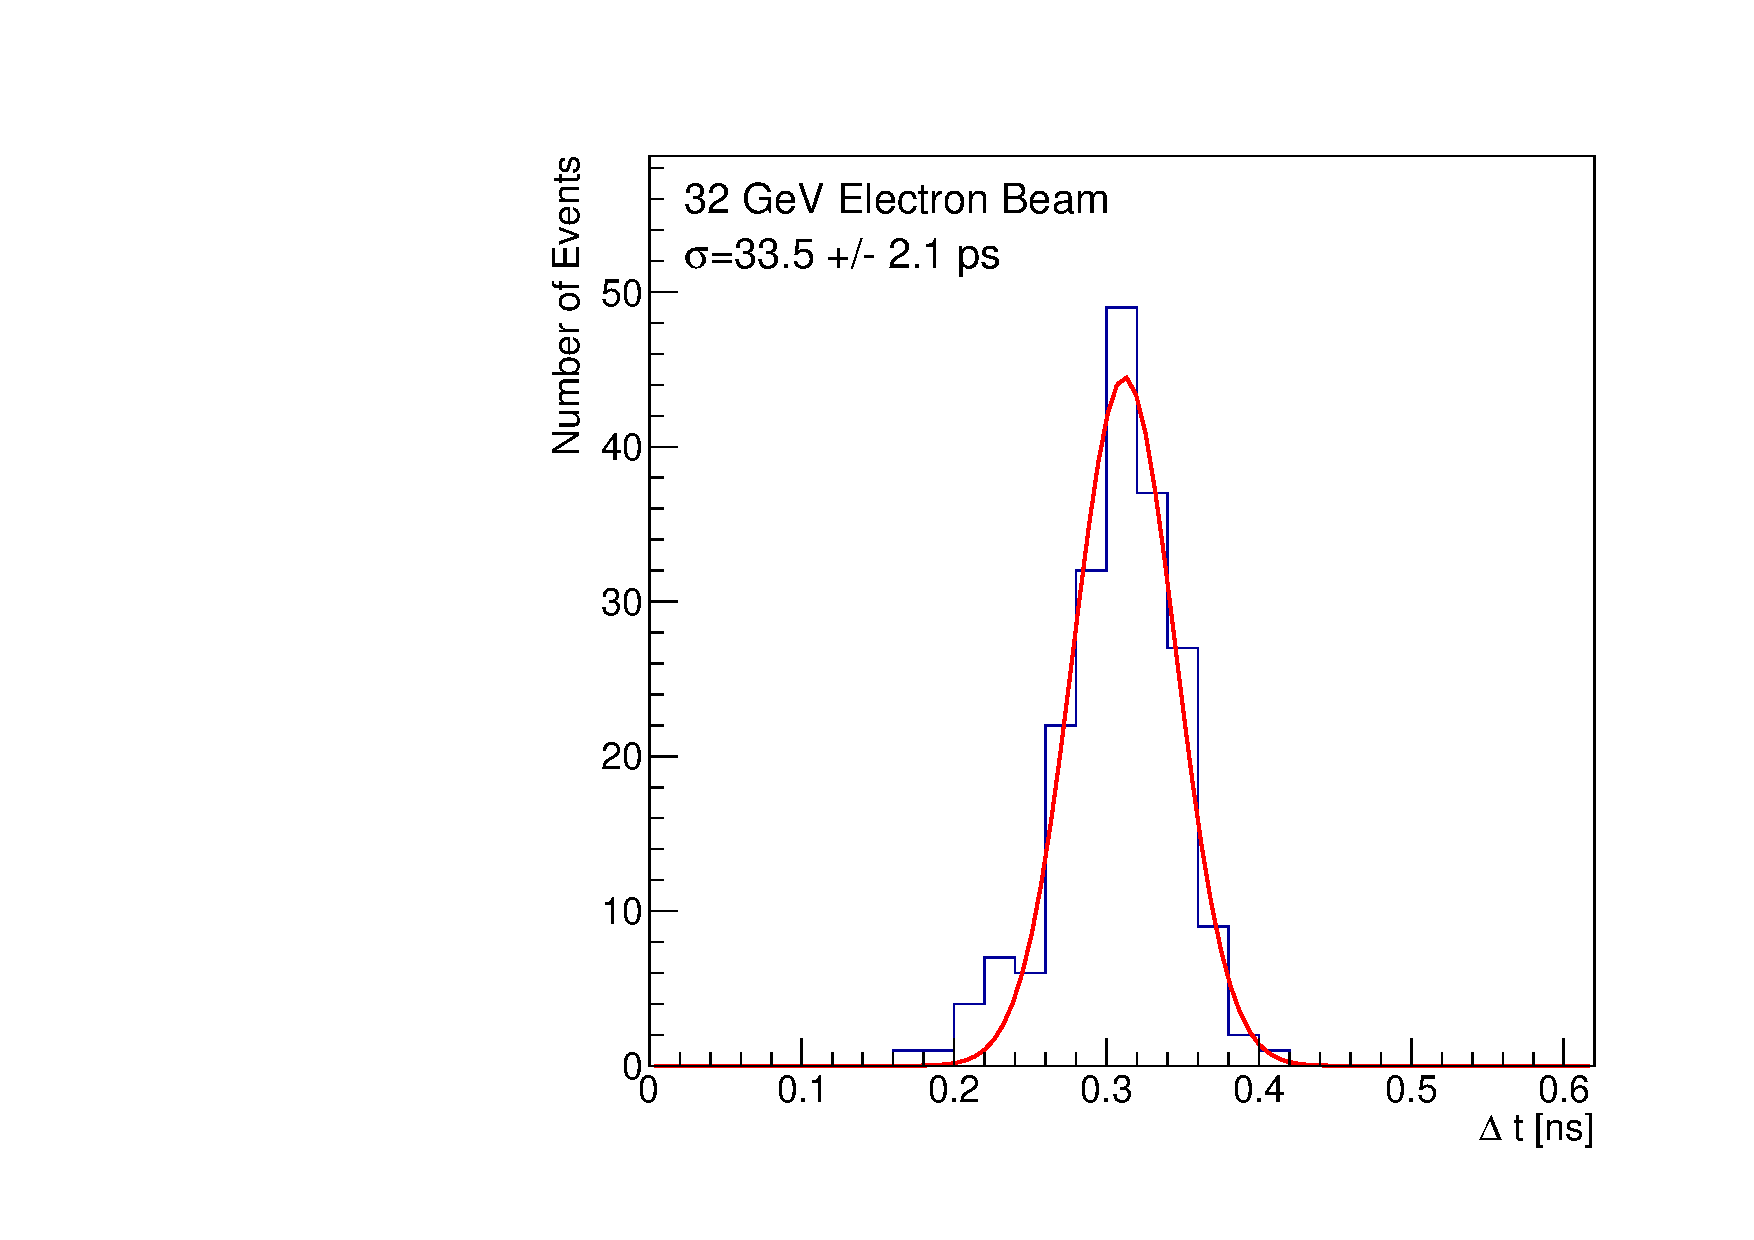
\includegraphics[width=0.23\textwidth]{figs/TOF_Electron_LYSOCube_32GeV} 
\caption{ \small Time of flight distributions for the LYSO cube sampling calorimeter
for 4 GeV (top left), 8 GeV(top right), 16 GeV (bottom left),  32 GeV (bottom right) electron beam energy. } 
\label{fig:LYSOCubeTOF}
\end{figure}

The time resolution measurement is plotted as a function of the
beam energy in Figure~\ref{fig:TOFResolutionVsEnergy} (left). We fit the result to the sum of a 
$1/\sqrt{E}$ term and a constant term of about $11$~ps.   Given that we measure the contribution 
to the intrinsic time resolution of the photodetector and the DAQ electronics to be about 
$20$~ps~\cite{MCPFastCaloNIMA}, using the results from the 32 GeV electron beam, we infer 
that the combined contribution to the time resolution from the shower profile
fluctuations, the scintillation mechanism, and the light propagation time inside the
LYSO cube is about $27$~ps.  

\subsection{Timing Studies of the LYSO-Tungsten Shashlik Calorimeter}
\subsubsection{Wavelength (WLS) shifting fibers readout (Y11, DSB1)}
We study the time resolution of a LYSO-tungsten Shashlik calorimeter, one of the
proposed choices for the Phase 2 upgrade of the CMS endcap calorimeter
system~\cite{Contardo:1605208}. We compare the time resolution performance for
two alternative light propagation schemes. 

In our setup the scintillation light is collected by WLS fibers that
pass through a set of four holes in the LYSO and tungsten layers. In 
Figure~\ref{fig:ShashlikDiagram}, a shashlik cell and the light extraction 
scheme is illustrated. A schematic diagram and a photograph showing this experimental
setup are shown in Figure~\ref{fig:ShashlikFiberSetup}. Two MCP-PMTs  by 
Hamamatsu (R3809) are used to collect the scintillation light, while a Photek 240 
MCP-PMT is used as a reference time detector. 

\begin{figure}[H] \centering
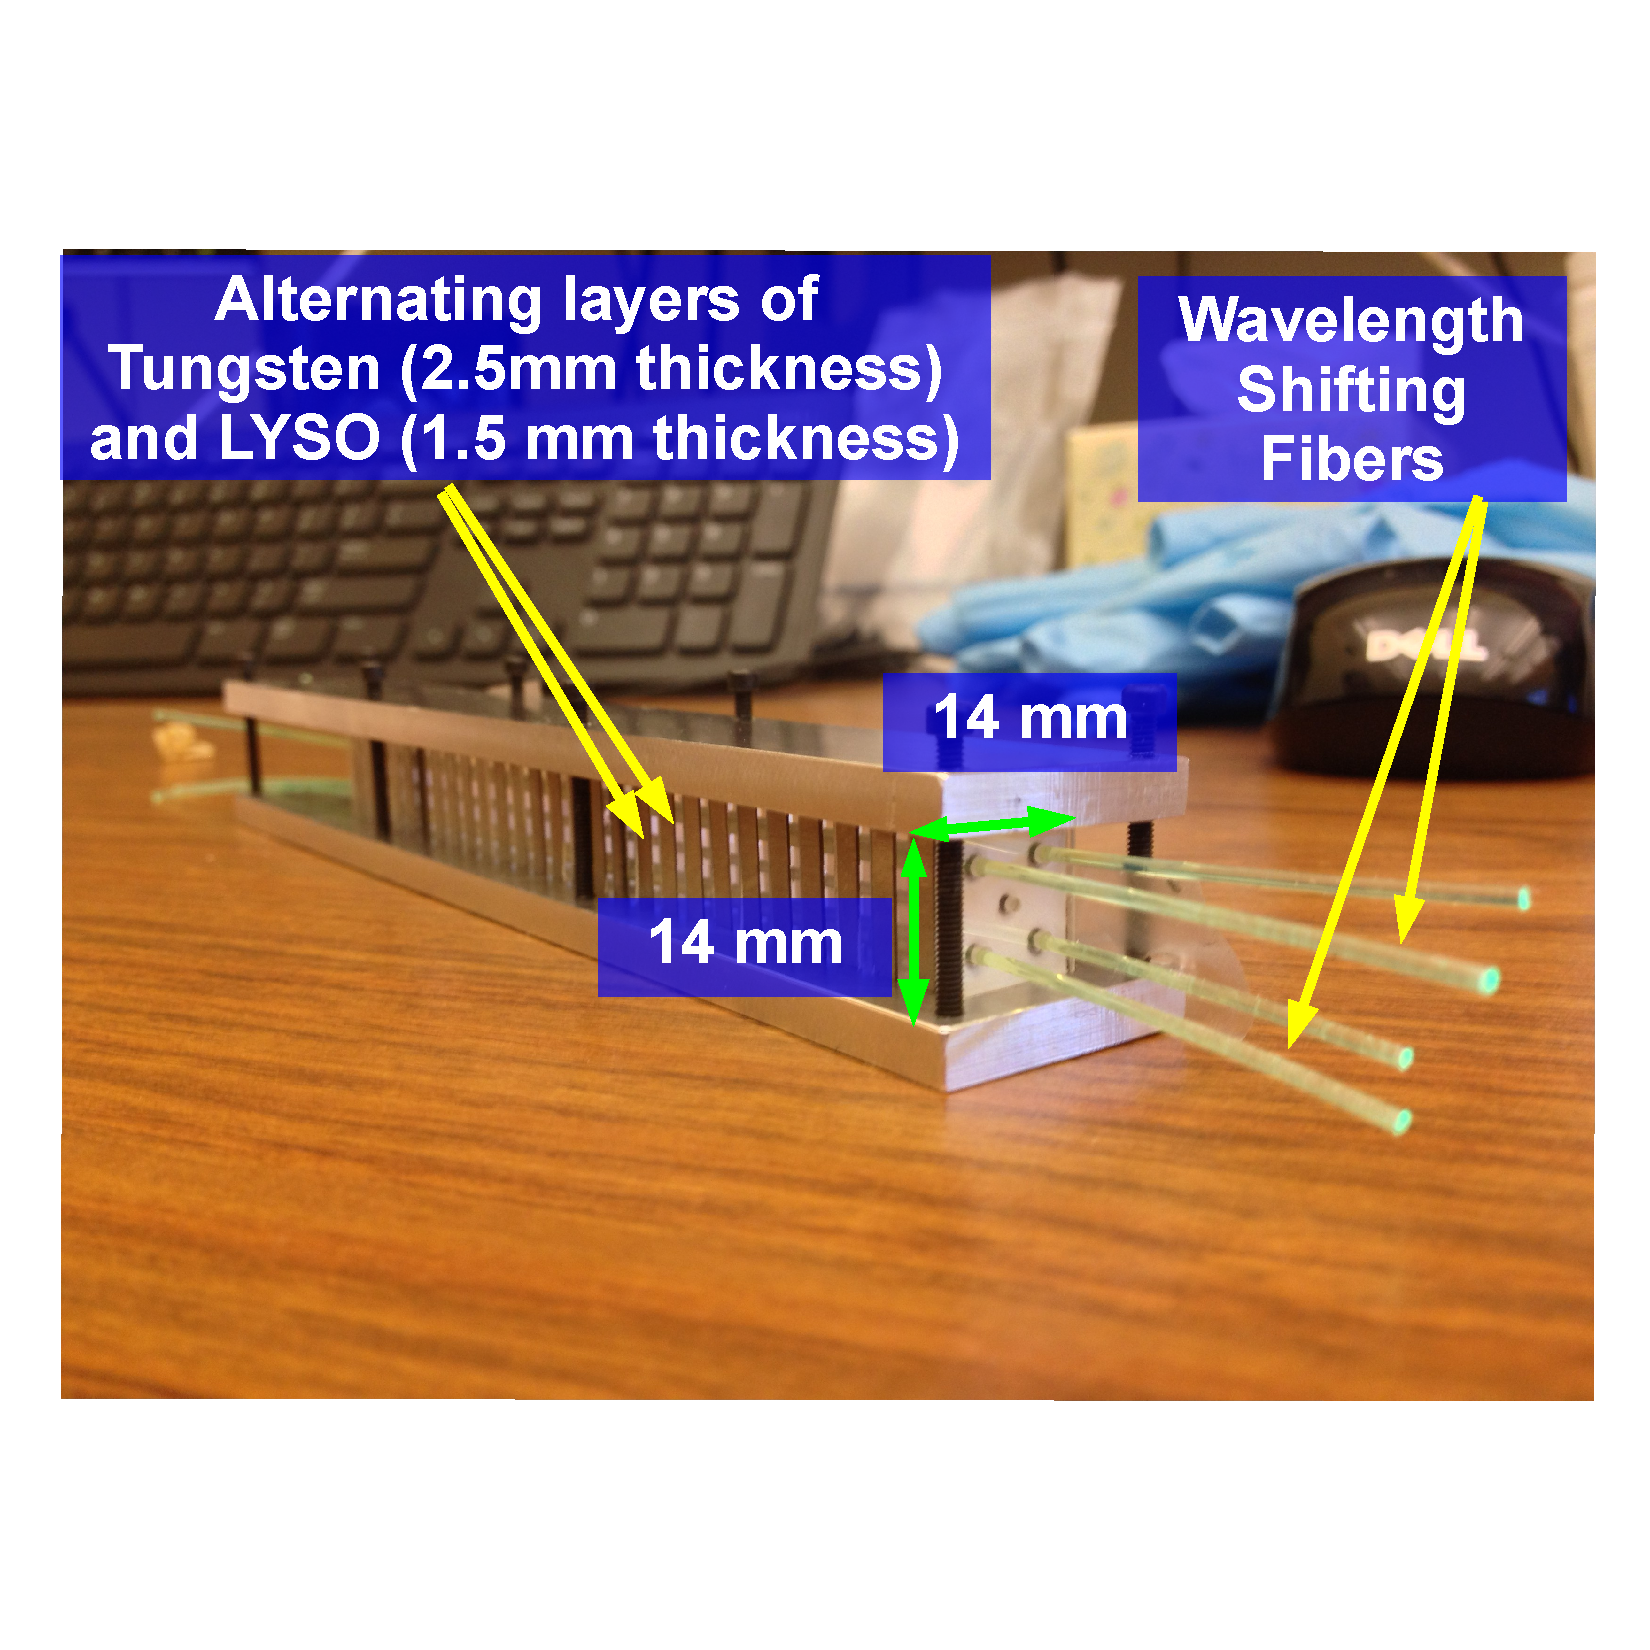
\includegraphics[width=0.6\textwidth]{figs/ShashlikCellPhoto.pdf} 
\caption{\small The shashlik configuration based upon interleaved W and LYSO layers. 
Twenty-eight LYSO crystal plates and twenty-seven W plates comprise the module.
Four WLS fibers are used to read out the scintillation light from the 
tiles. } 
\label{fig:ShashlikDiagram}
\end{figure}

\begin{figure}[H] \centering
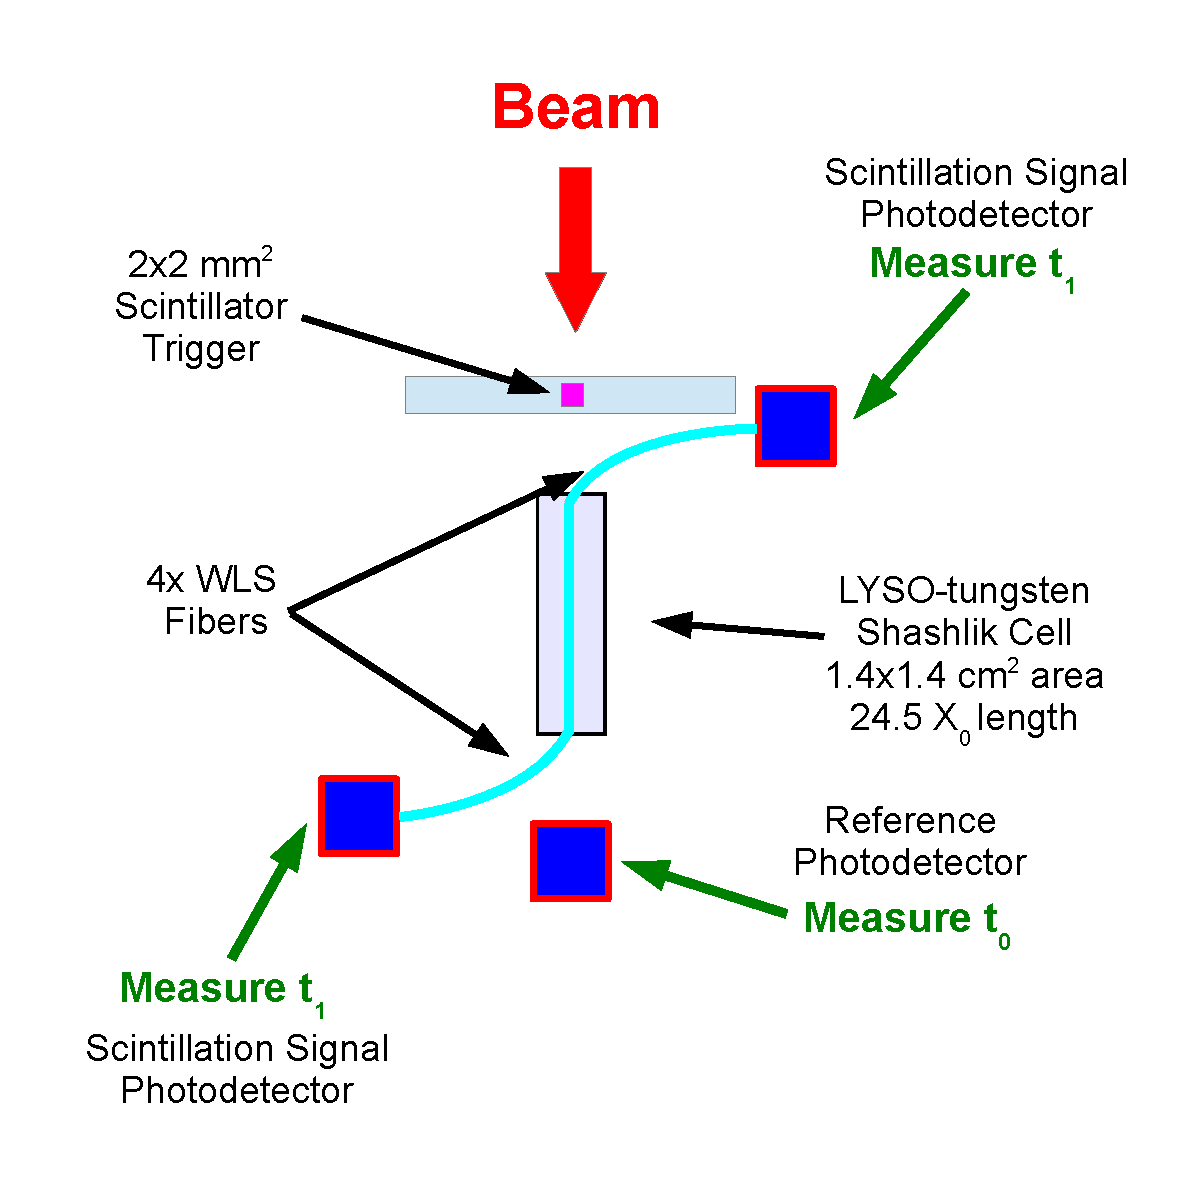
\includegraphics[width=0.45\textwidth]{figs/ShashlikFiberSetupSchematic} 
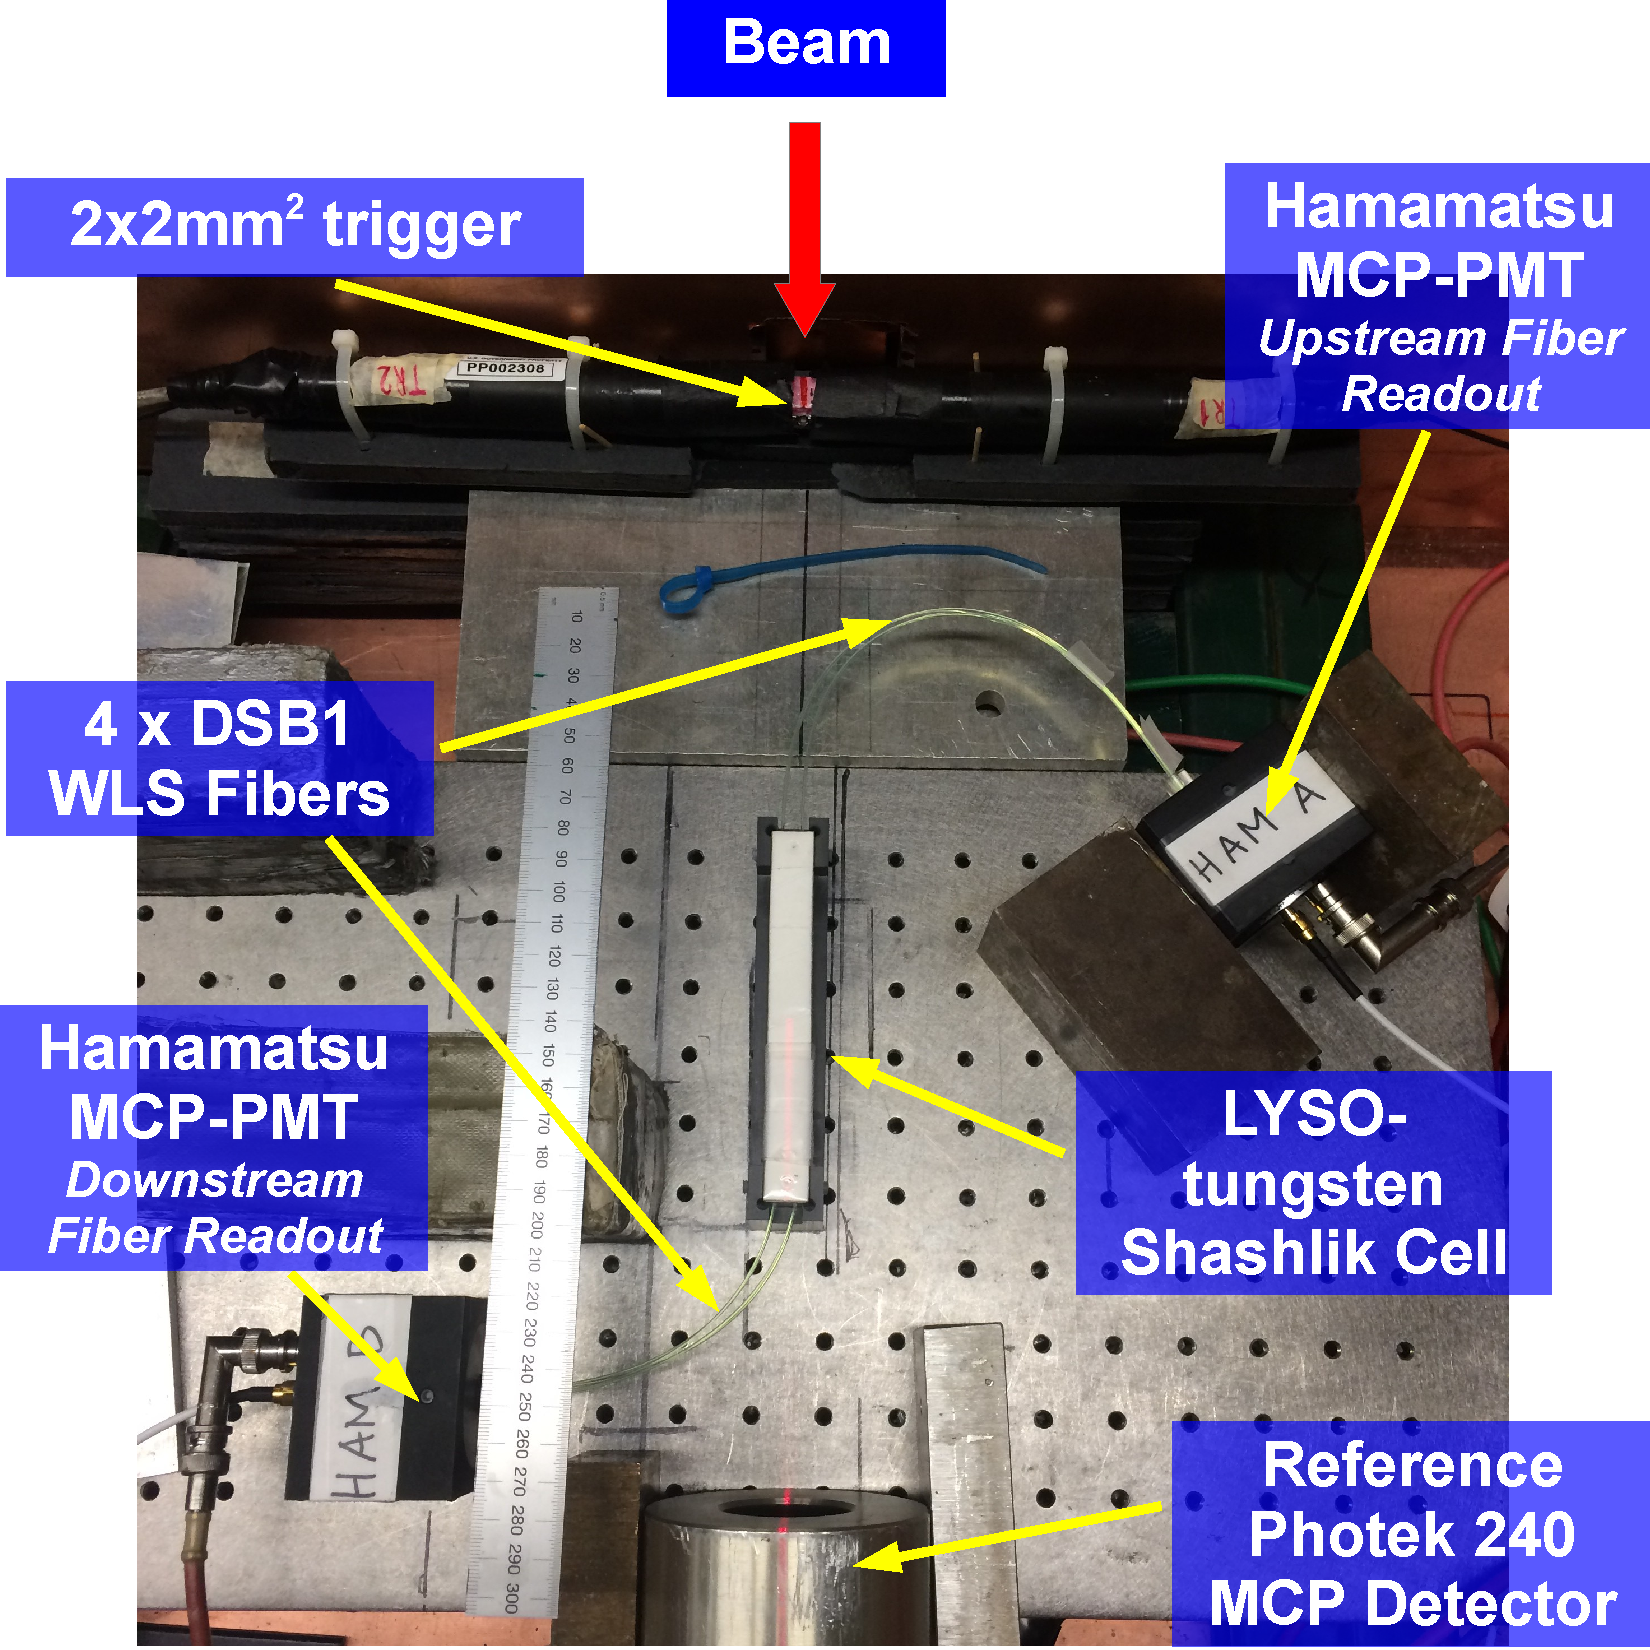
\includegraphics[width=0.45\textwidth]{figs/ShashlikFiberSetupPhoto} 
\caption{\small A schematic diagram of the experimental setup for the
time of flight measurement using the LYSO-tungsten shashlik calorimeter
with fiber signal extraction, along with a photograph of the
experimental setup. } 
\label{fig:ShashlikFiberSetup}
\end{figure}

%In this setup the wavelength shifting mechanism in the fibers affects the rise
%time and time jitter of the final signal pulse.
 %We investigate this effect in
%greater detail by 
 We compare the signal pulses obtained using two different
 types of WLS fiber in the same LYSO-tungsten shashlik calorimeter. In
 Figure~\ref{fig:FiberPulseComparison} (a) and (b) and we show the pulse shapes
 averaged over a few hundred events obtained using DSB1 fibers~\cite{Albrecht}
 and Y11 fibers, plotted in blue and red respectively. We find that the rise
 time of the pulse obtained using the DSB1 fibers, about $2.4$~ns, is
 significantly faster than the rise time of the pulse obtained using the Y11
 fibers, which is about $7.1$~ns. To optimize the time resolution of this type
 of calorimeter the DSB1 fiber provides a better choice than Y11 if only this
 parameter is considered. The signal rise times we observe are comparable to the
 measured decay times of the corresponding WLS fibers~\cite{Albrecht}. 
 
% compared
% with the average pulse shape obtained from direct optical coupling of the
% photodetector to the edge of one of the LYSO tiles, plotted in green. 
%


\begin{figure}[H] \centering
%\includegraphics[width=0.32\textwidth]{figs/FiberPulsesY11DSB1} 
%
%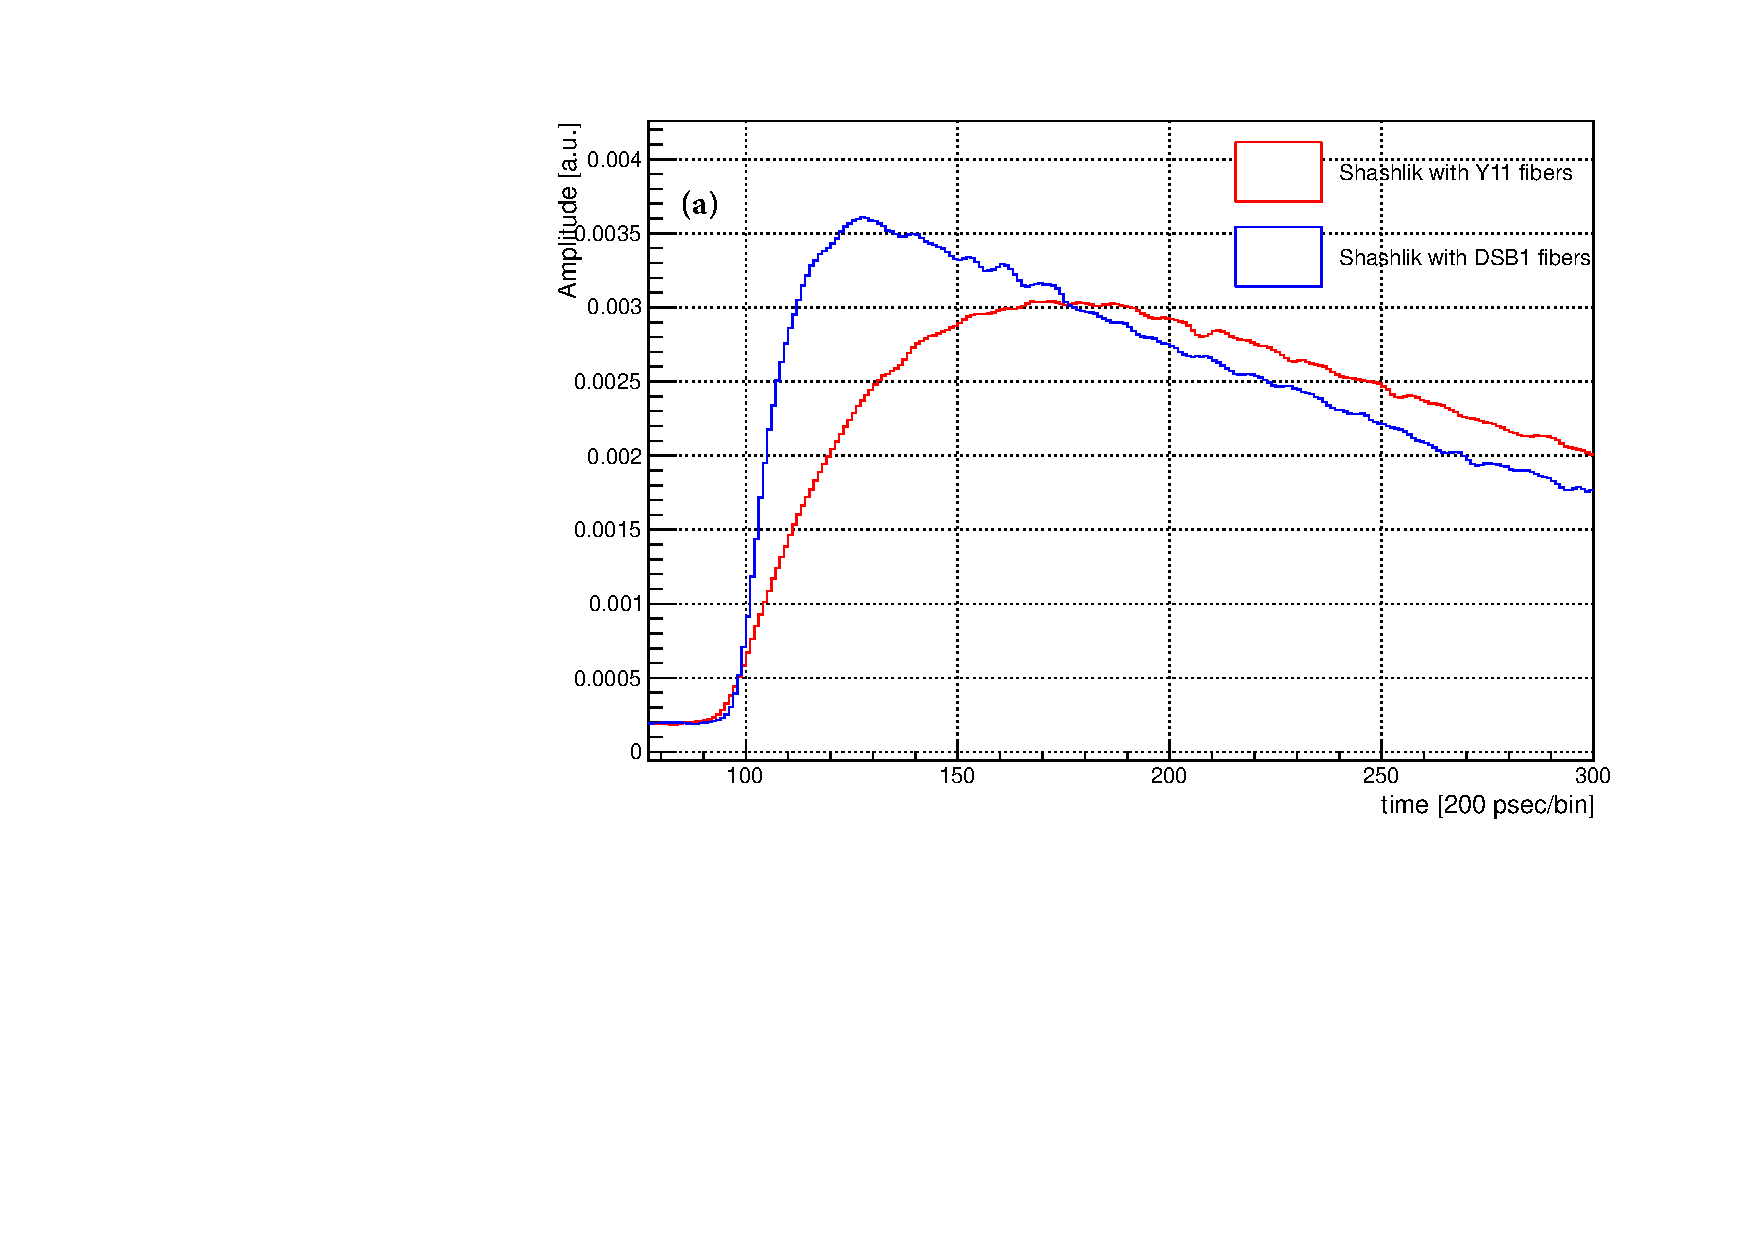
\includegraphics[width=0.32\textwidth]{figs/FiberPulsesZoomY11DSB1} 
%
%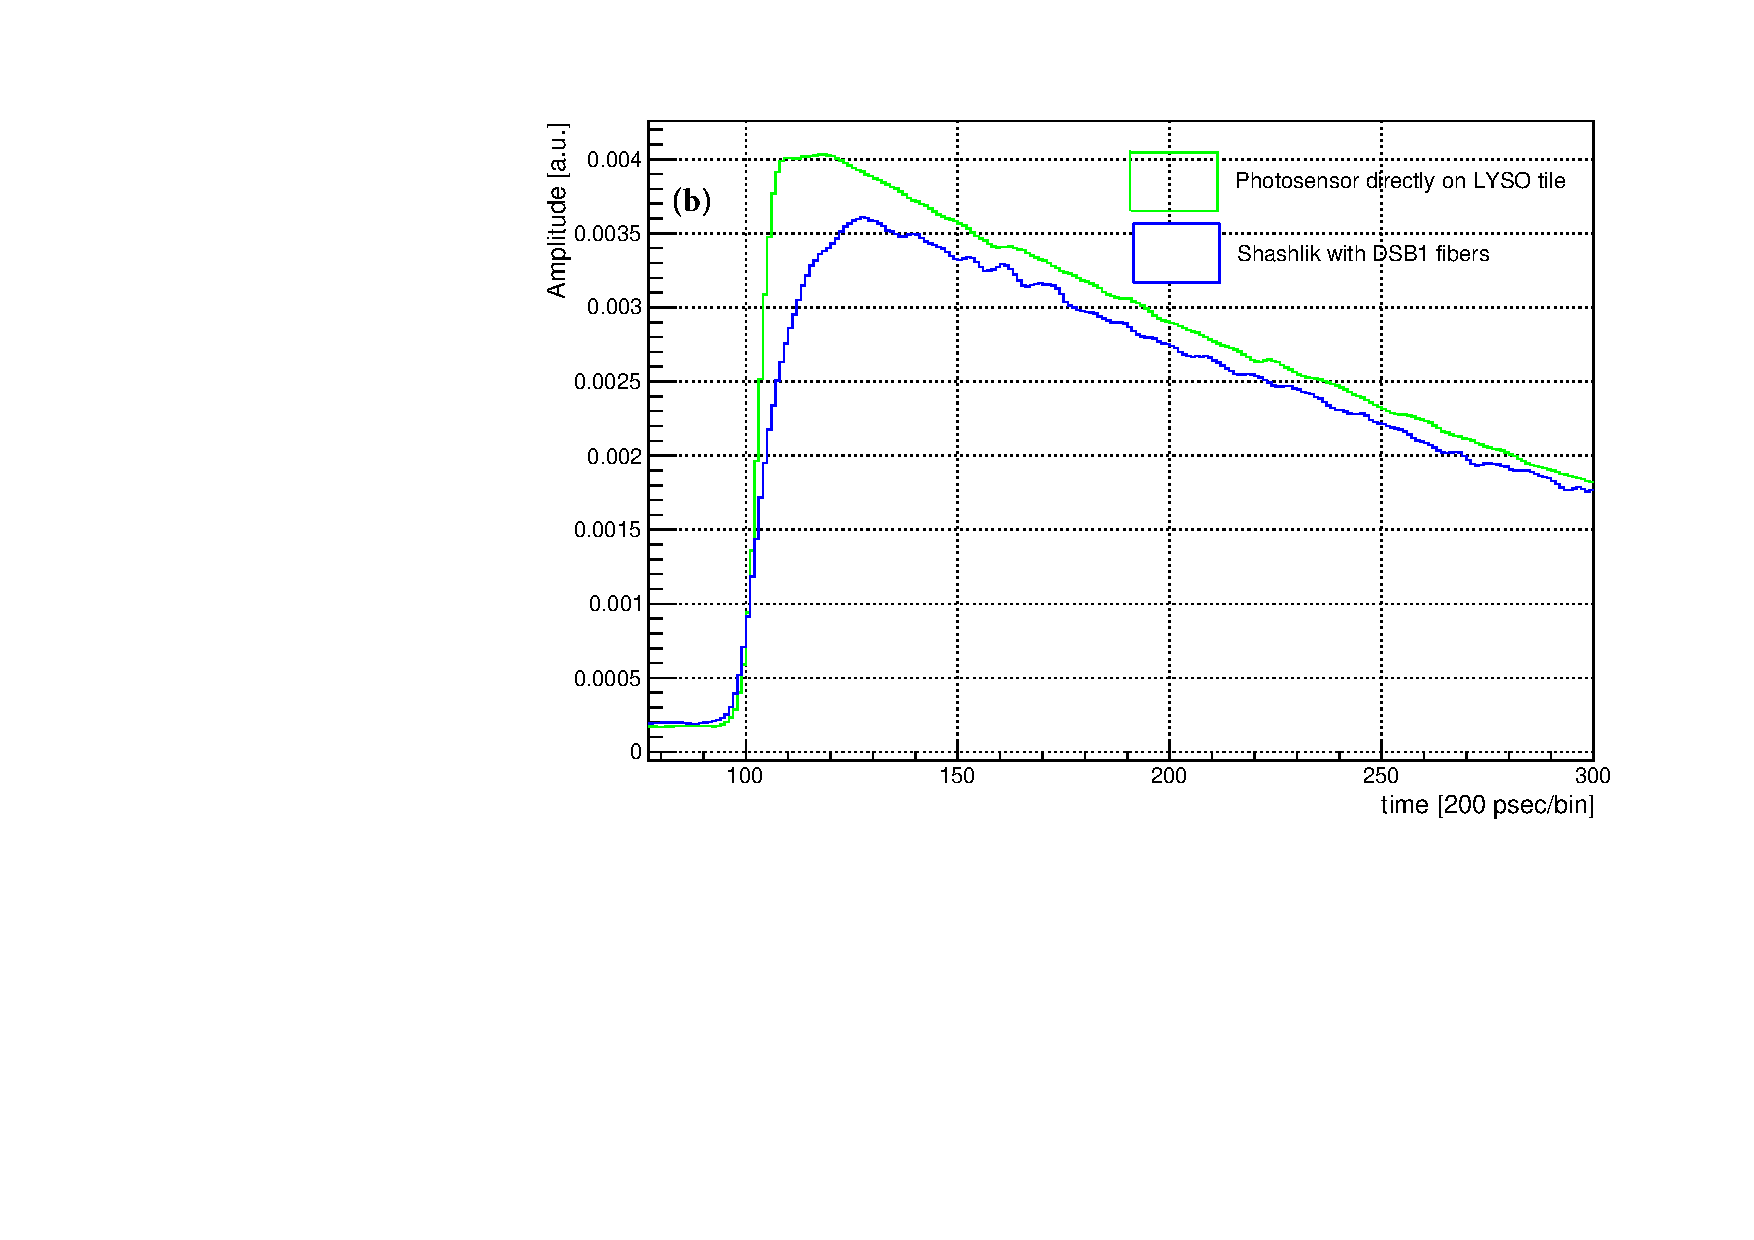
\includegraphics[width=0.32\textwidth]{figs/FiberPulsesZoomDirectDSB1} 
%
\caption{\small (a) Pulse shapes digitized by the DRS4 board and averaged over several hundred events 
obtained from the LYSO-tungsten shashlik calorimeter with light extracted using
DSB1 (blue) and Y11 (red) WLS fibers. 
(b) A zoomed-in version of the figure (a). (c)  DSB1(blue) shashlik average light pulse shape compared with 
the averaged pulse shape obtained from direct optical coupling of the photodetector to one edge of  a LYSO tile in the shashlik calorimeter.  (green)} 
\label{fig:FiberPulseComparison}
\end{figure}


Using the shashlik calorimeter cell with DSB1 fibers, we measure the time resolution
for electron beams with energy varying between $4$~GeV and $32$~GeV.
In Figure~\ref{fig:ShashlikFiberEnergy32GeV}(b) we show the distribution
of the pulse integral which is proportional to the total collected charge,
for the $32$~GeV beam, and observe an energy resolution of about $5\%$
while for the small LYSO cube shown in ~\ref{fig:ShashlikFiberEnergy32GeV} (a),  the energy 
resolution was about 20\%. For this particular run in the Shashlik setup, no electron identification 
requirements could be made due to a misconfiguration of the upstream Cherenkov counter, 
so the background is visible.


Time of flight distributions, fitted to gaussian functions,
are shown in Figure~\ref{fig:ShashlikFiberTOF}, and the 
$\sigma$ parameter of the gaussian fit is plotted as a function of the
beam energy in Figure~\ref{fig:ShashlikSideReadoutTOFResolutionVsEnergy}.
We find that the dependence of the time resolution on
beam energy follows a $1/\sqrt{E}$ functional form, indicating
that the current calorimeter setup remains in the photostatistics limited regime. 
The best time resolution we obtain with this setup is $104$~ps. As the measurements are 
photostatistics limited, the result can be improved in the future if the light collection
efficiency is increased.


\begin{figure}[H] \centering
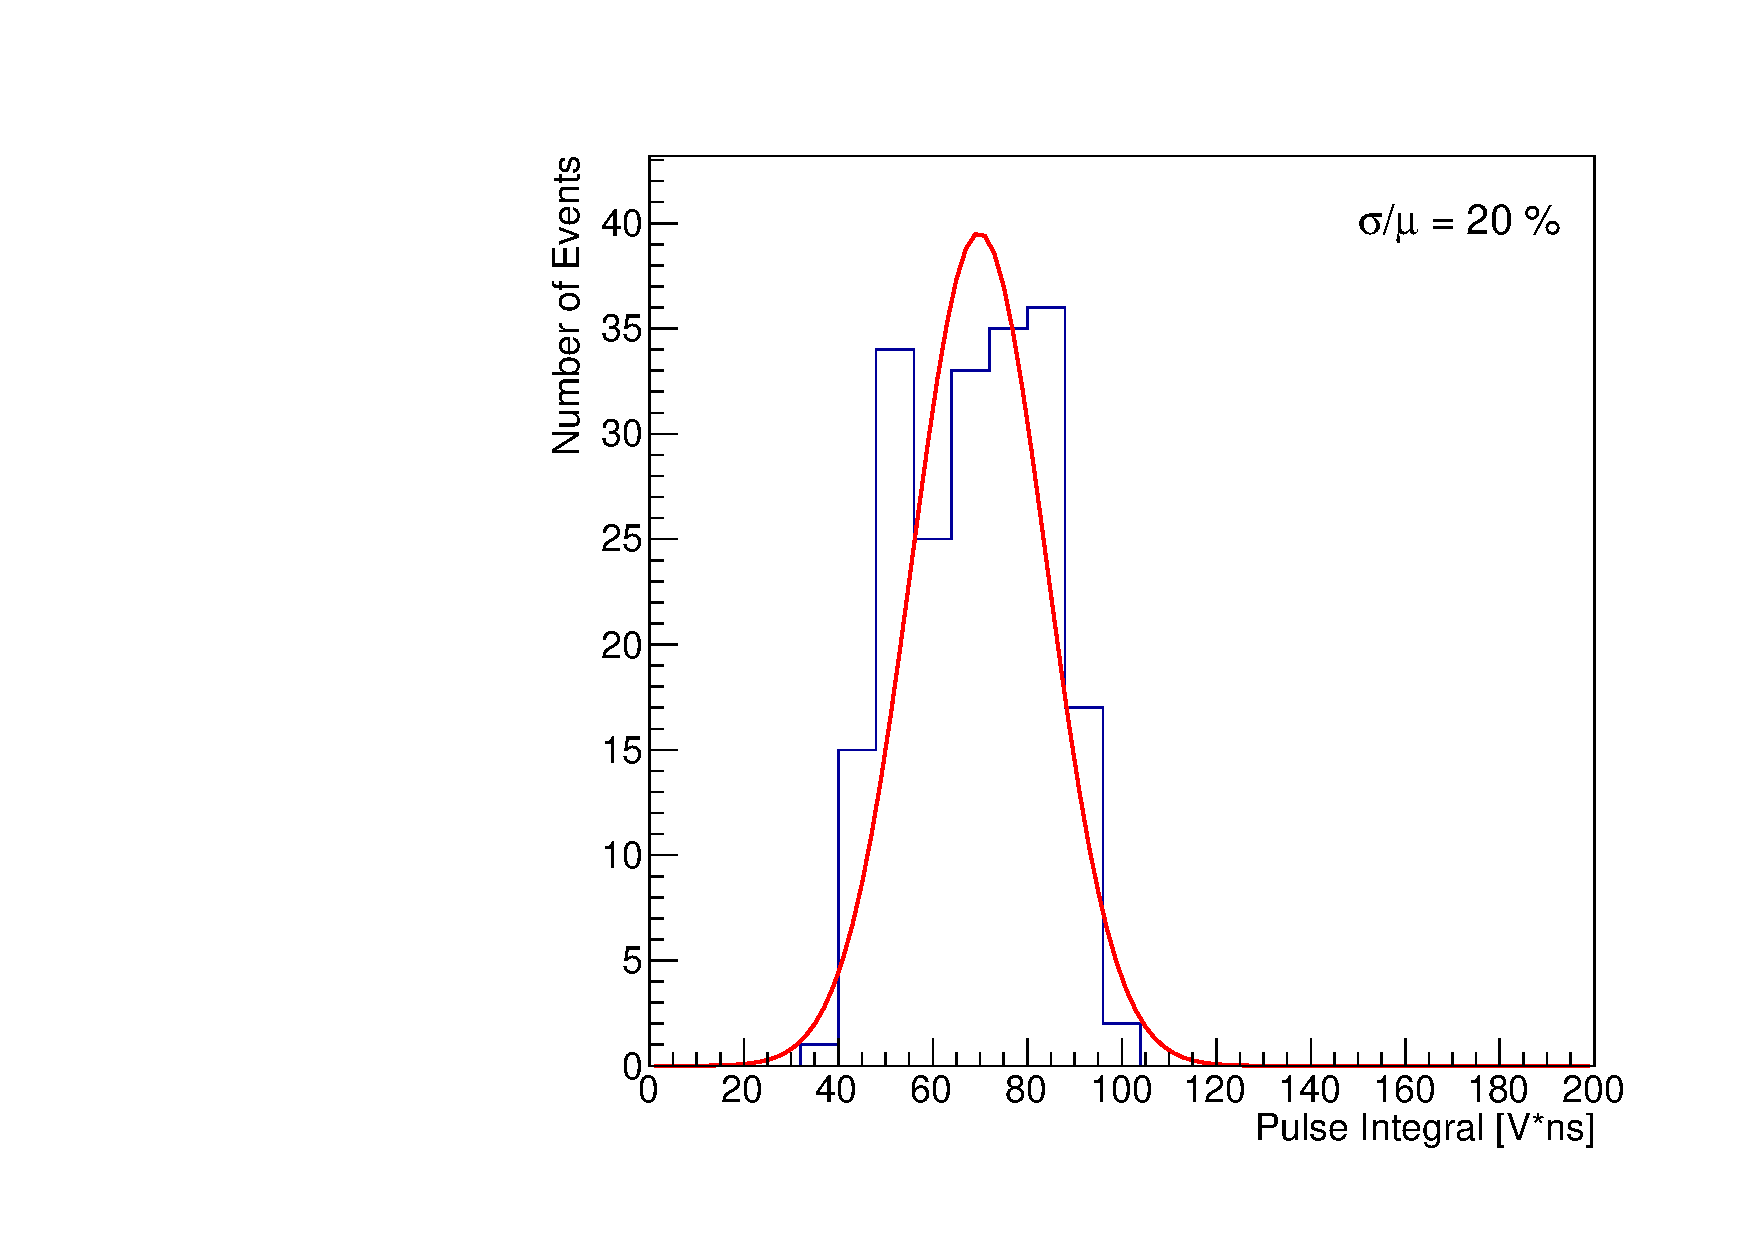
\includegraphics[width=0.45\textwidth]{figs/TOF_Electron_LYSOCube_32GeV_energy} 
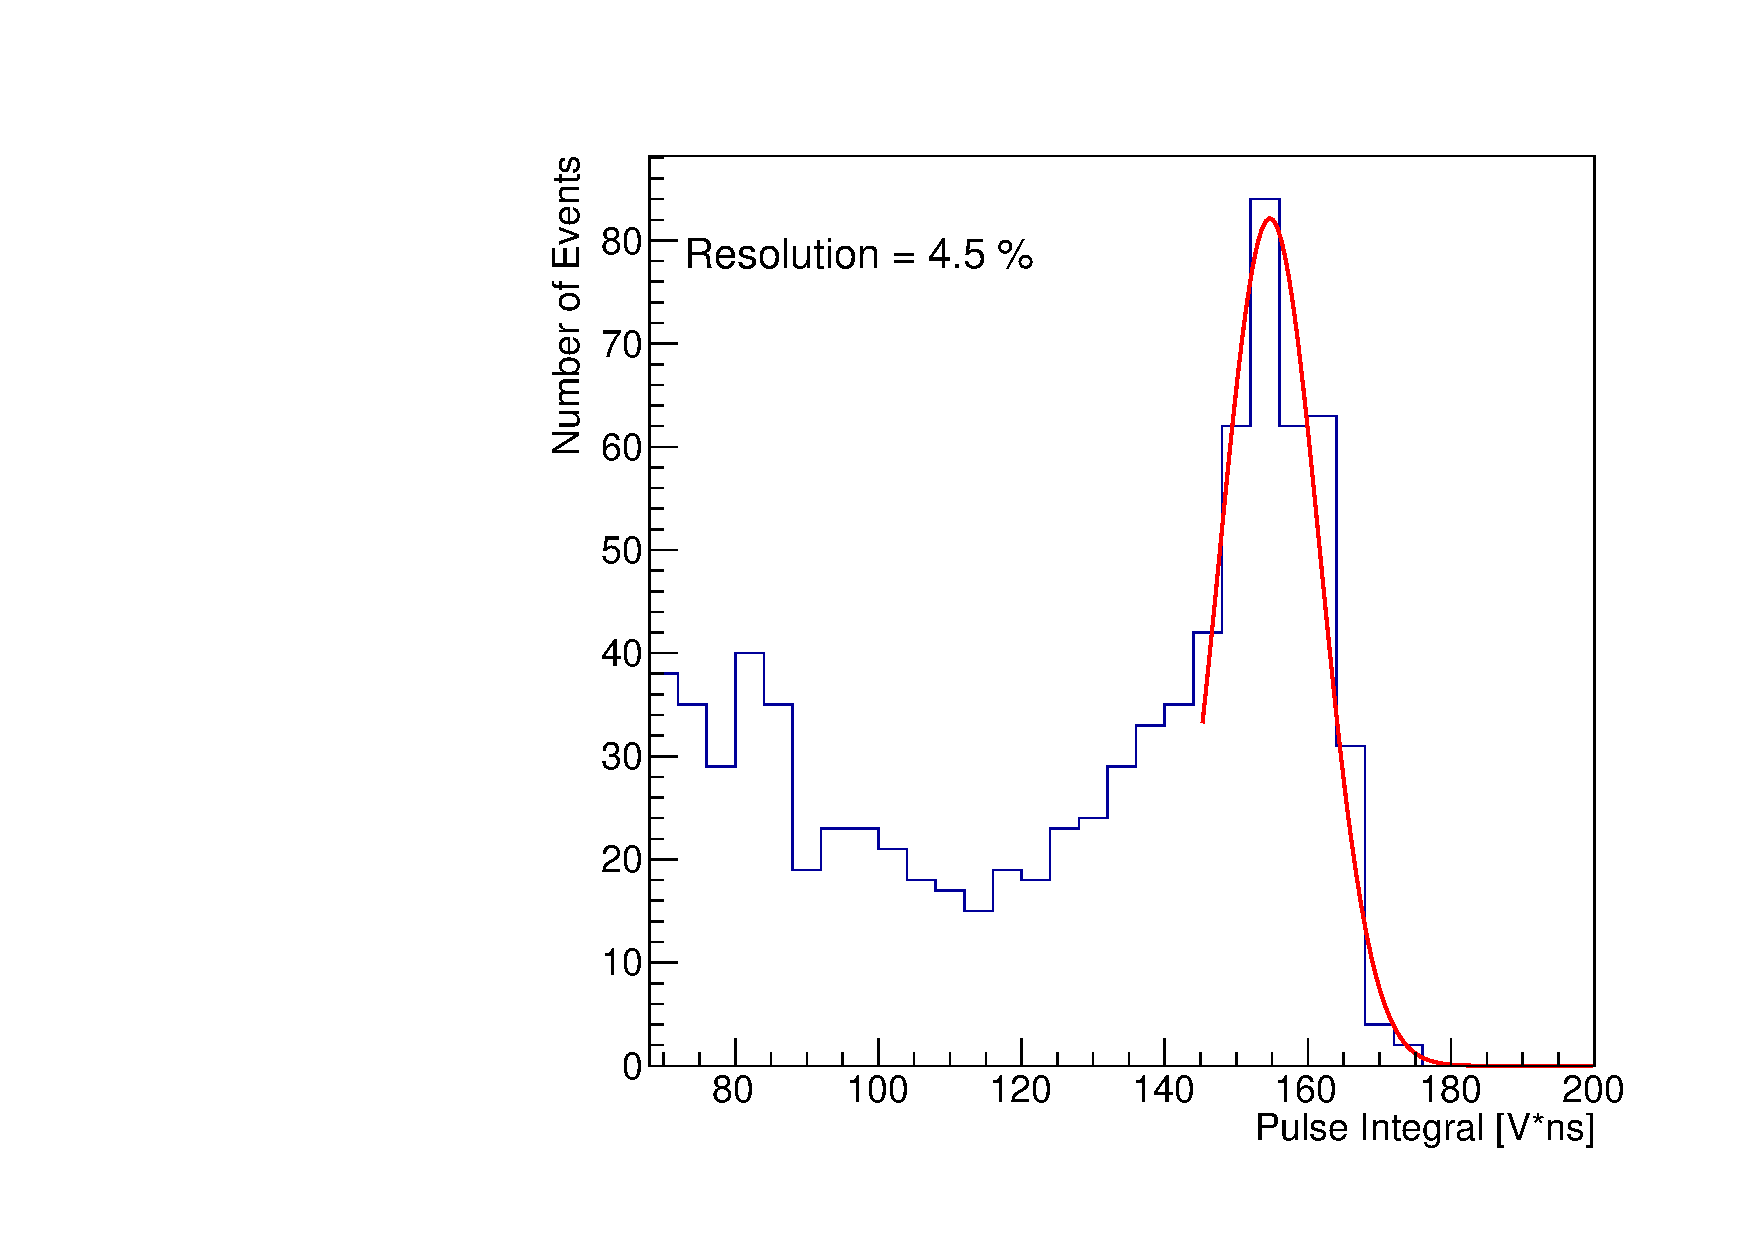
\includegraphics[width=0.45\textwidth]{figs/TOF_ShashlikDSB1Fiber_Electron_32GeV_energy} 
\caption{ (Left) Histogram of the pulse integral which is proportional to the
total collected charge is shown for events recorded using the LYSO cube sampling
calorimeter for a $32$~GeV electron beam. (Right) Histogram of the pulse
integral for events recorded using the LYSO-tungsten shashlik calorimeter using
DSB1 fibers, for a $32$~GeV electron beam. The background is included due to a
misconfiguration of the Cherenkov counter. } 
\label{fig:ShashlikFiberEnergy32GeV}
\end{figure}



\begin{figure}[H] \centering
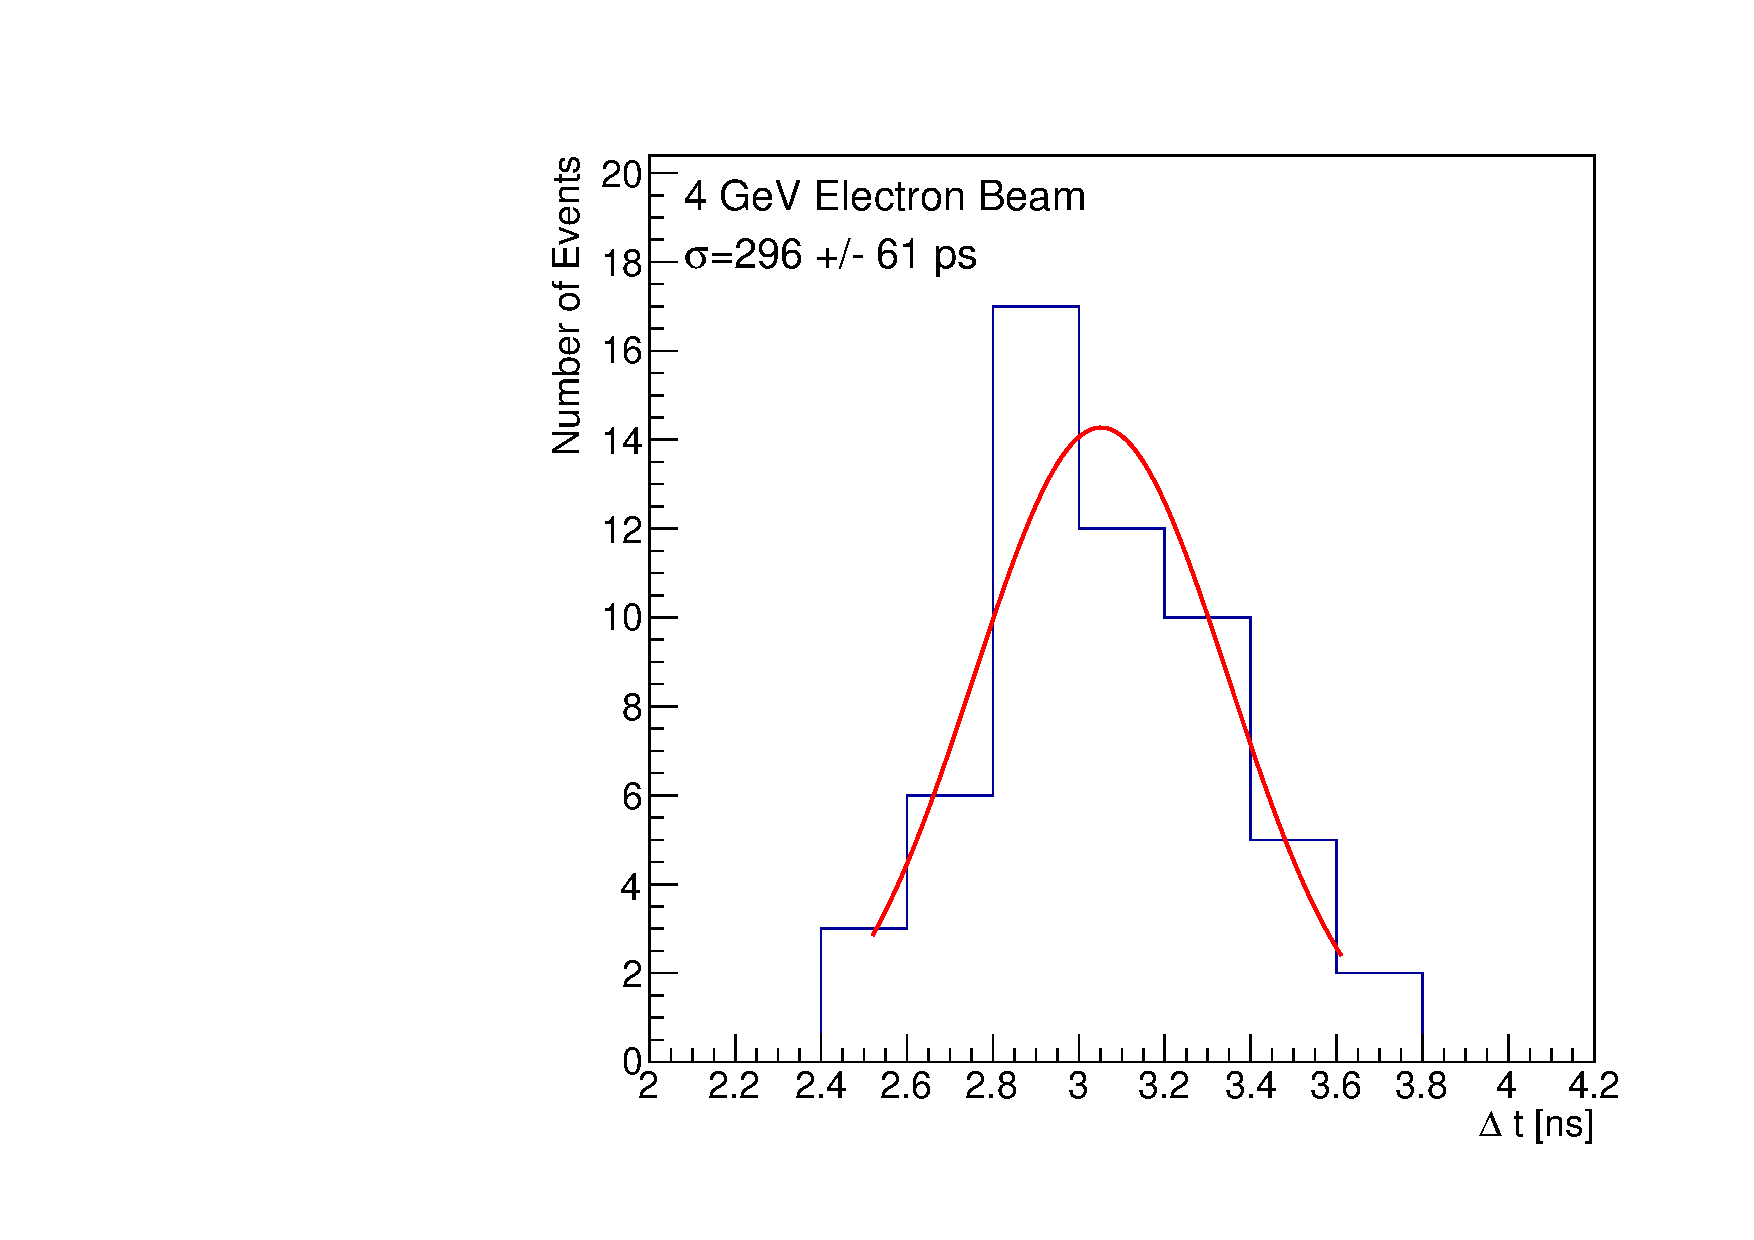
\includegraphics[width=0.23\textwidth]{figs/TOF_ShashlikDSB1Fiber_Electron_4GeV} 
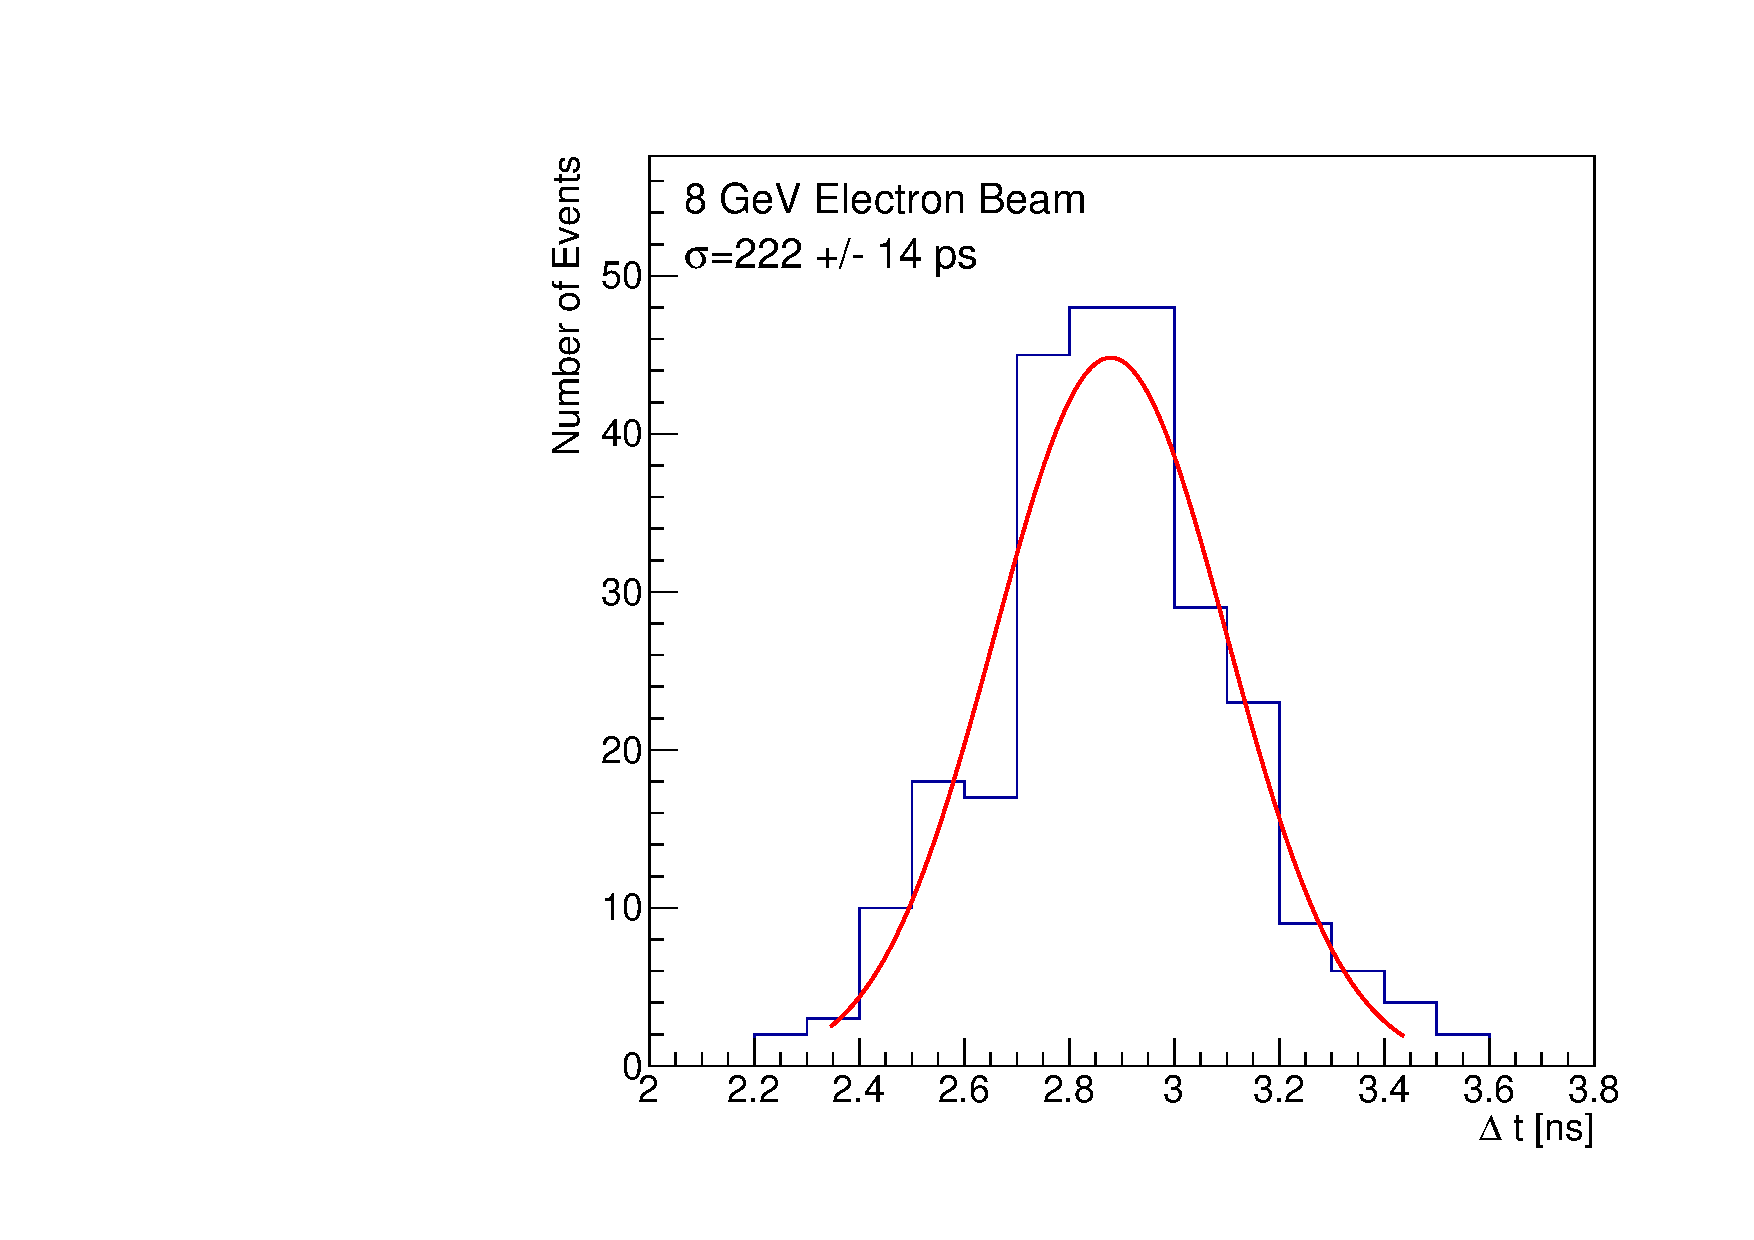
\includegraphics[width=0.23\textwidth]{figs/TOF_ShashlikDSB1Fiber_Electron_8GeV} 
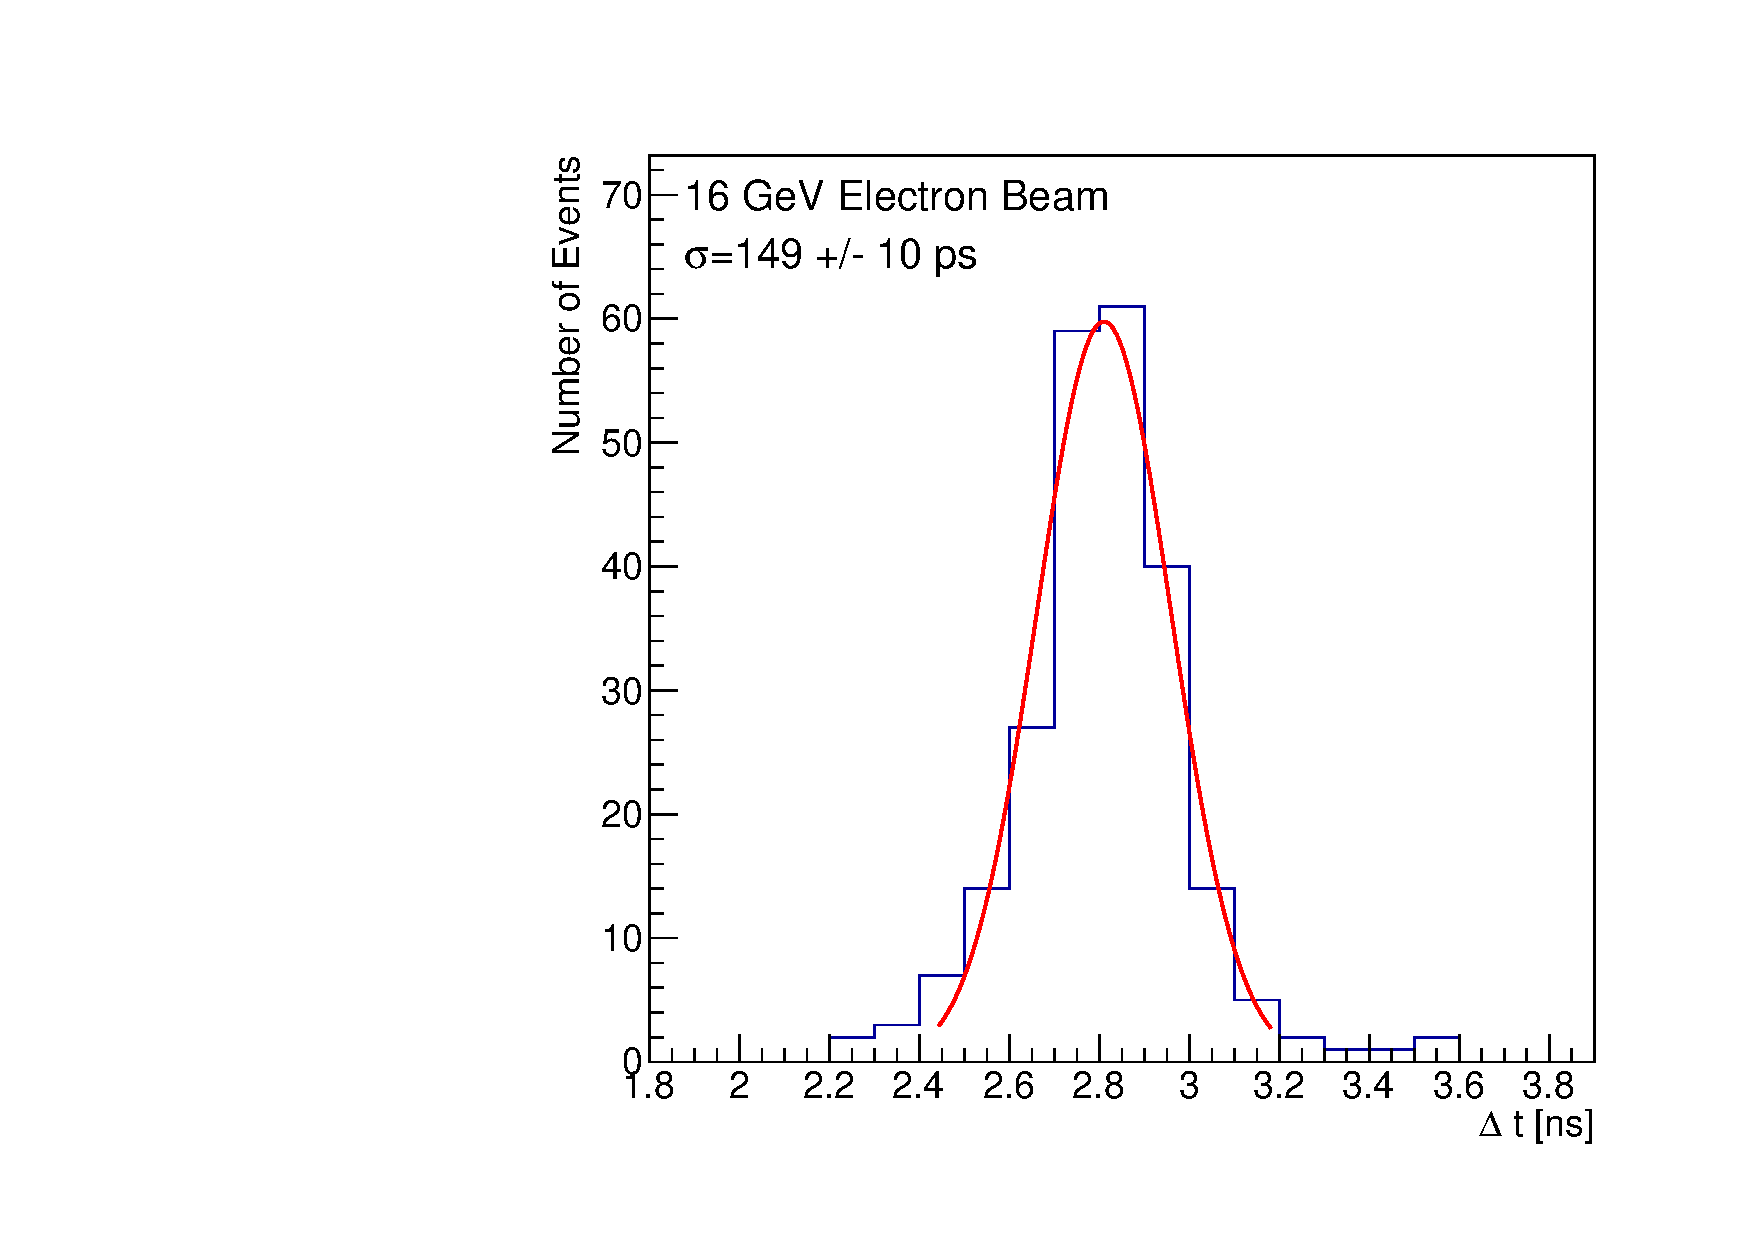
\includegraphics[width=0.23\textwidth]{figs/TOF_ShashlikDSB1Fiber_Electron_16GeV} 
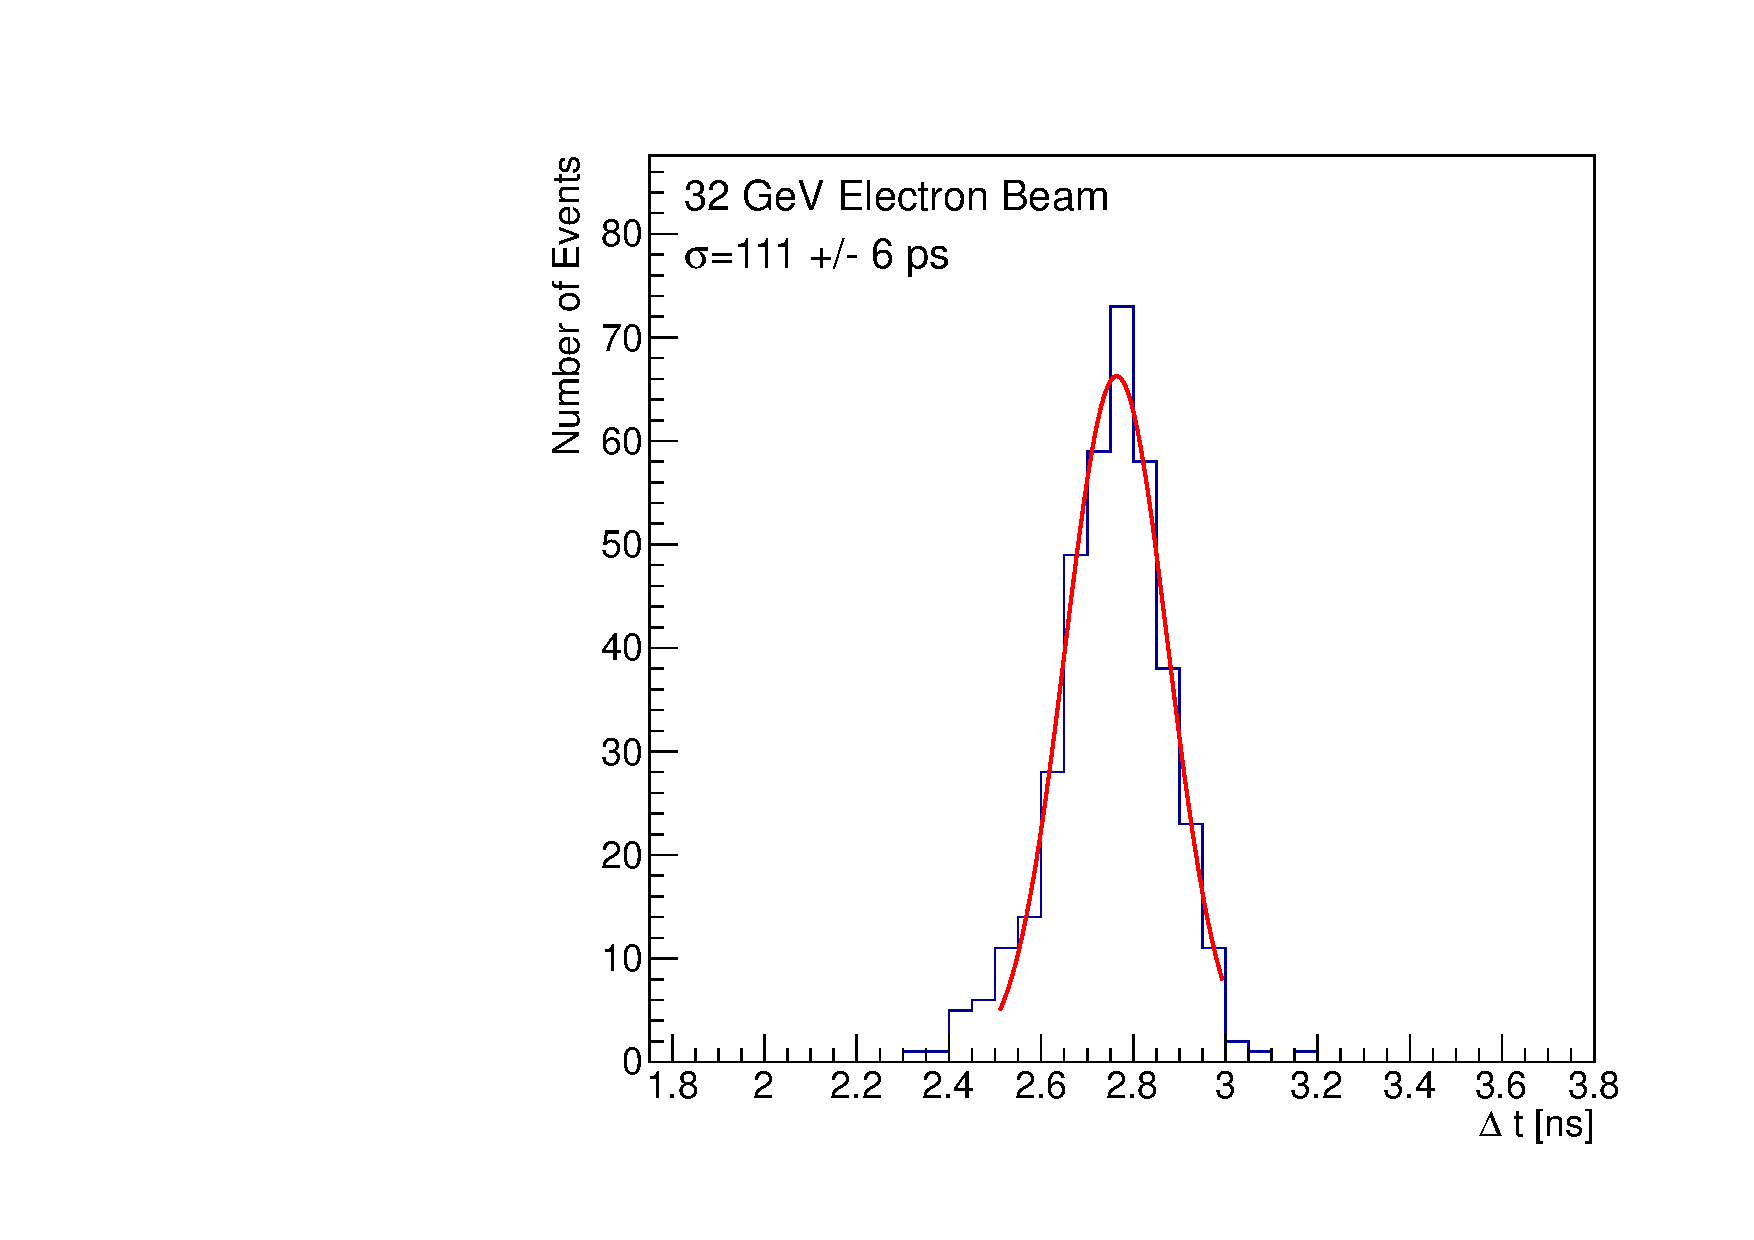
\includegraphics[width=0.23\textwidth]{figs/TOF_ShashlikDSB1Fiber_Electron_32GeV} 
\caption{\small Time of flight distributions for the LYSO-tungsten shashlik calorimeter
using DSB1 fibers for electron beams with varying beam energies.} 
\label{fig:ShashlikFiberTOF}
\end{figure}


\subsubsection{Directly coupled MCP-PMTs to LYSO shashlik plates}

In this setup the MCP-PMT photodetectors are directly coupled to the edges of two adjacent LYSO layers in the shashlik
calorimeter and scintillation light is directly transported to the photodetector
through the edges of the tile layers. A schematic diagram and corresponding
picture  of the experimental setup are shown in
Figure~\ref{fig:ShashlikSideReadoutSetup}. In
Figure~\ref{fig:ShashlikSideReadoutExposedLayersPhoto}, we show a zoomed-in
photograph of the exposed LYSO plates from which the scintillation light signal
is extracted.

\begin{figure}[H] \centering
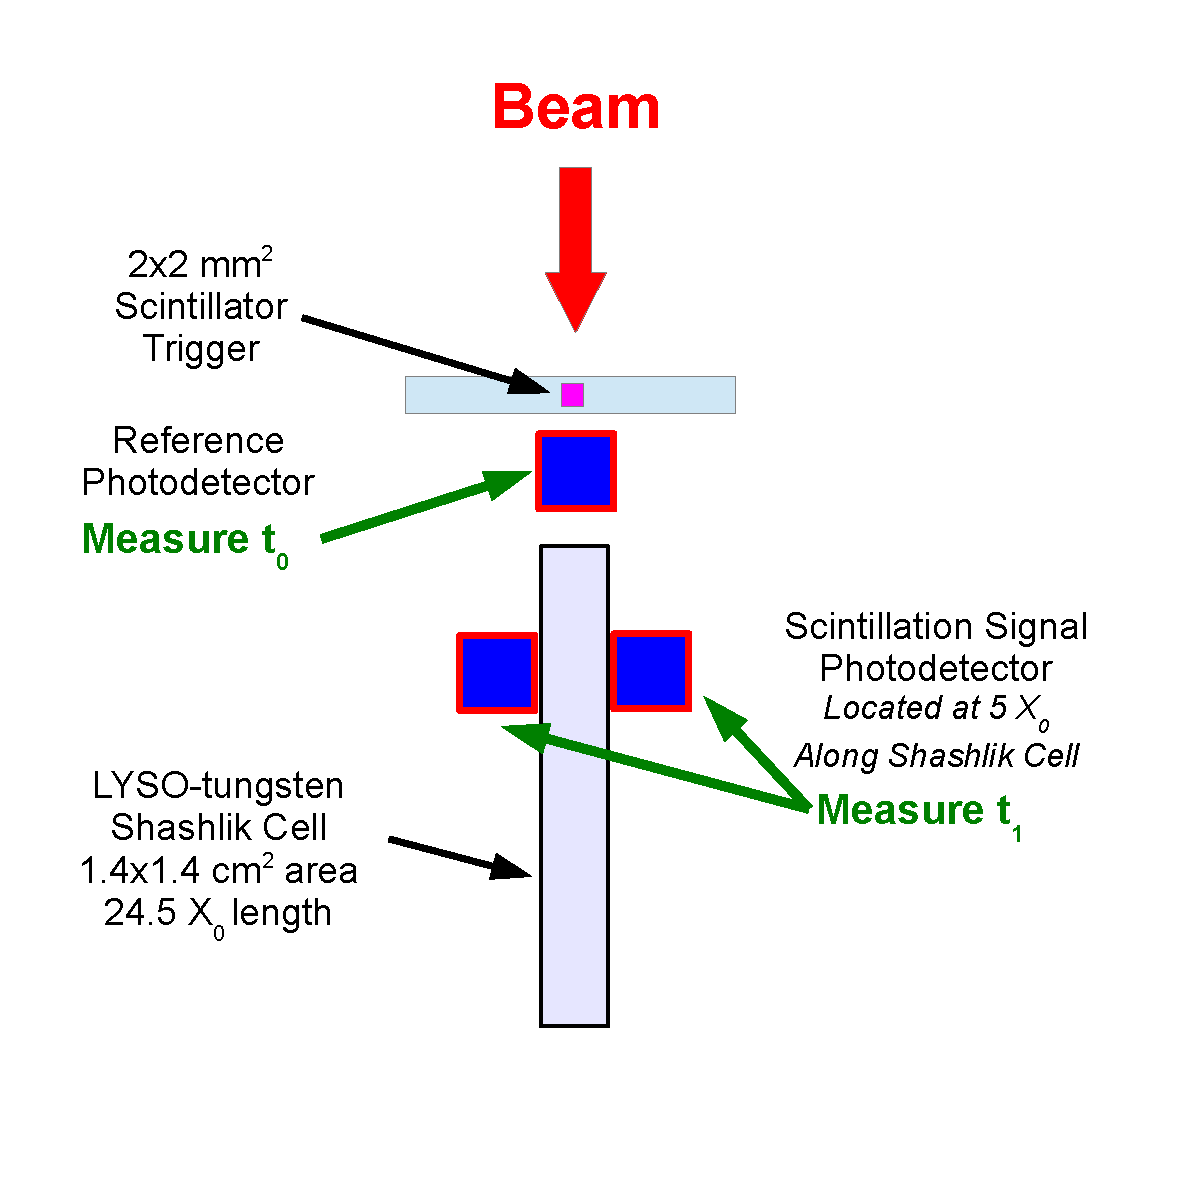
\includegraphics[width=0.45\textwidth]{figs/ShashlikSideReadoutSetupSchematic} 
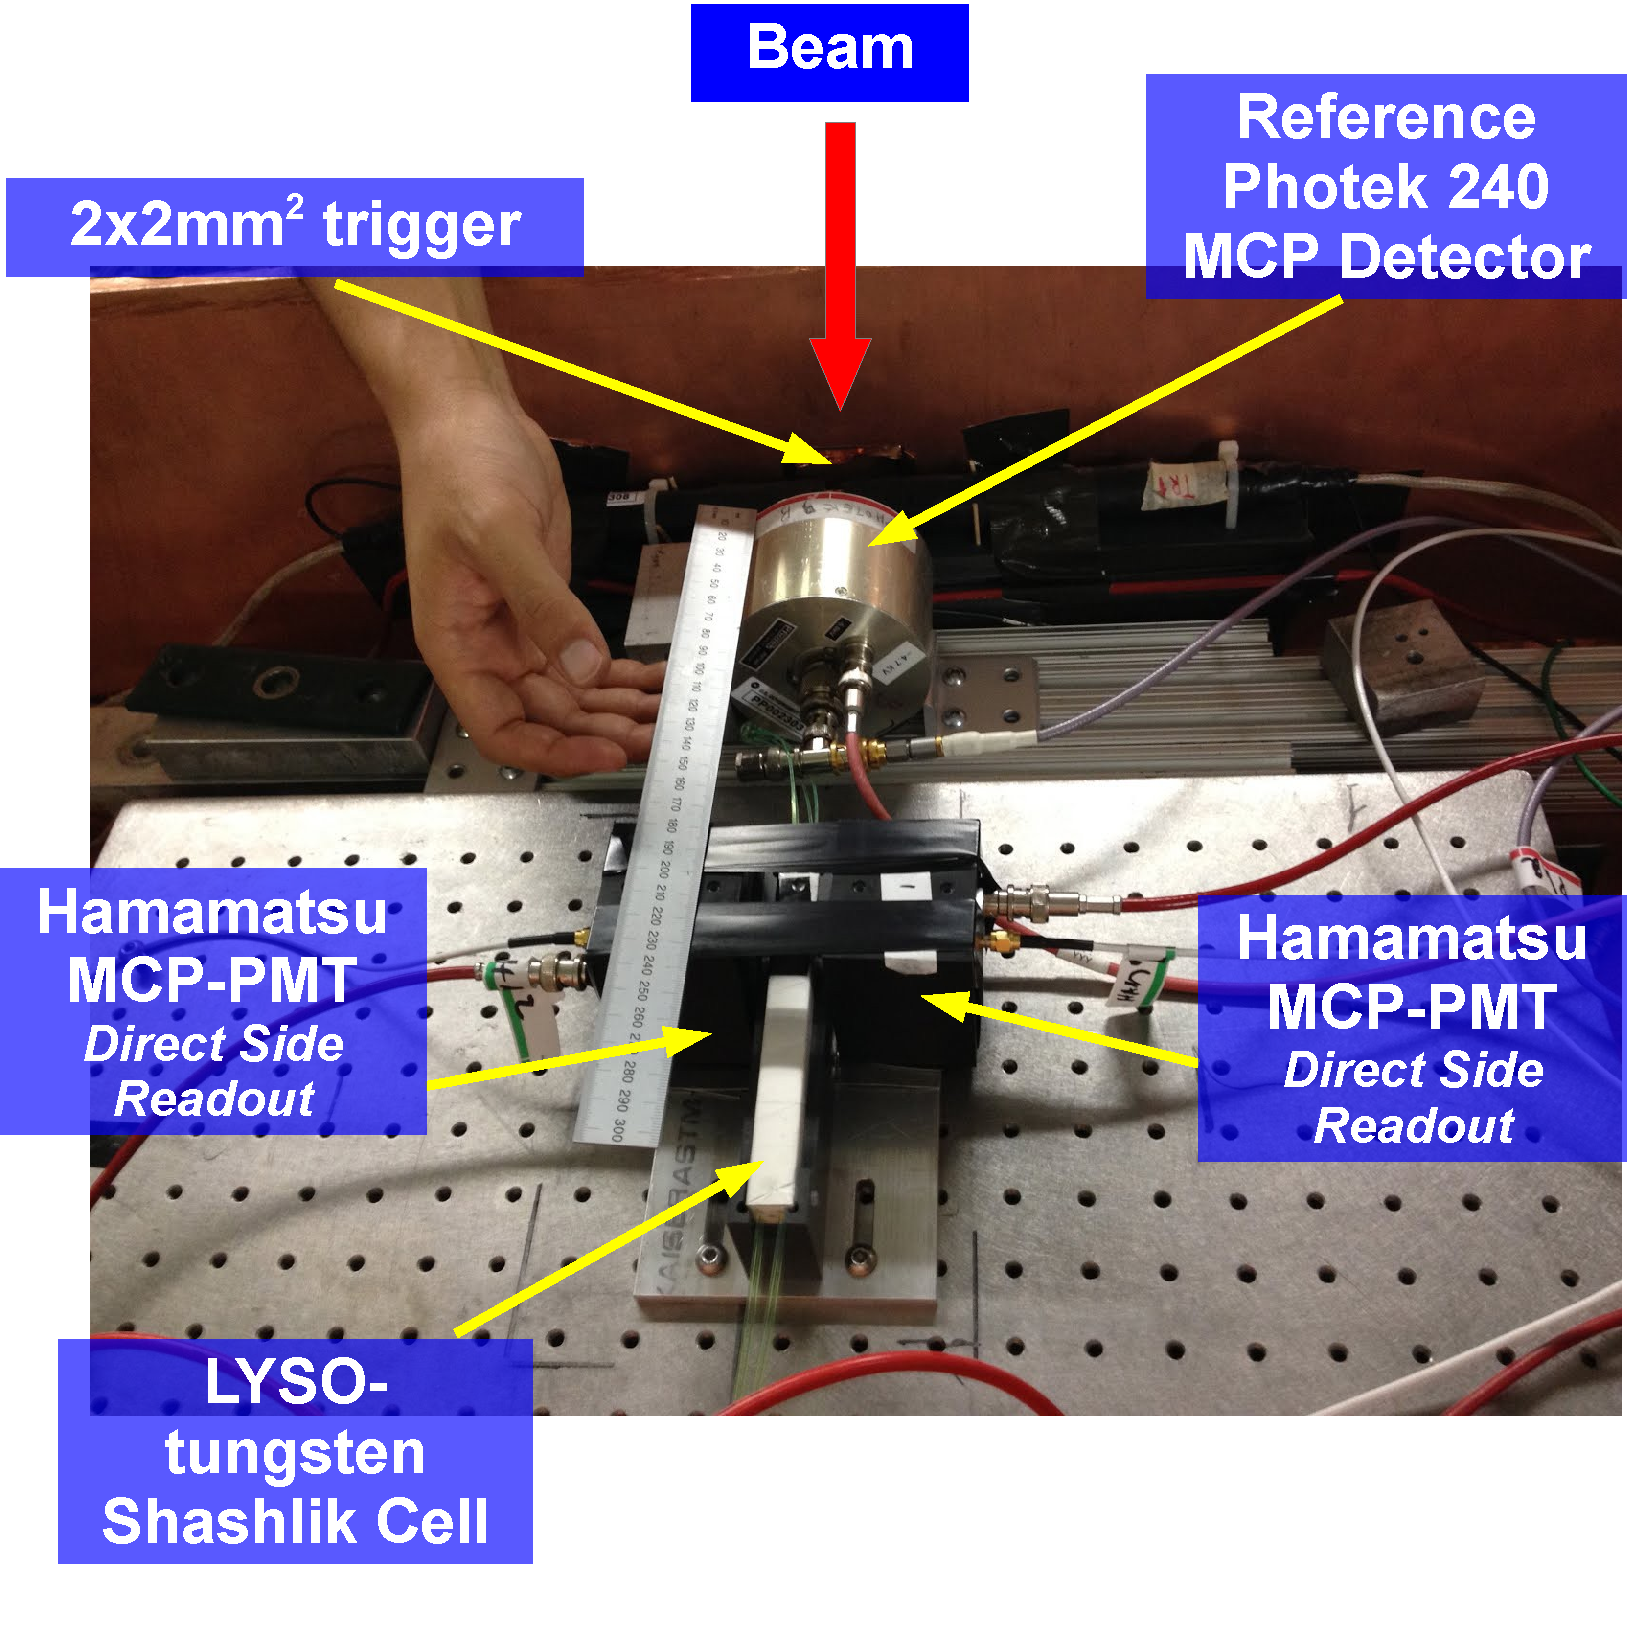
\includegraphics[width=0.45\textwidth]{figs/ShashlikSideReadoutPhotoB} 
\caption{ \small A schematic diagram of the experimental setup for the
time of flight measurement using the LYSO-tungsten shashlik calorimeter
with signal extraction from the edges of two LYSO plates, along
with a picture of the experimental setup. } 
\label{fig:ShashlikSideReadoutSetup}
\end{figure}

\begin{figure}[H] \centering
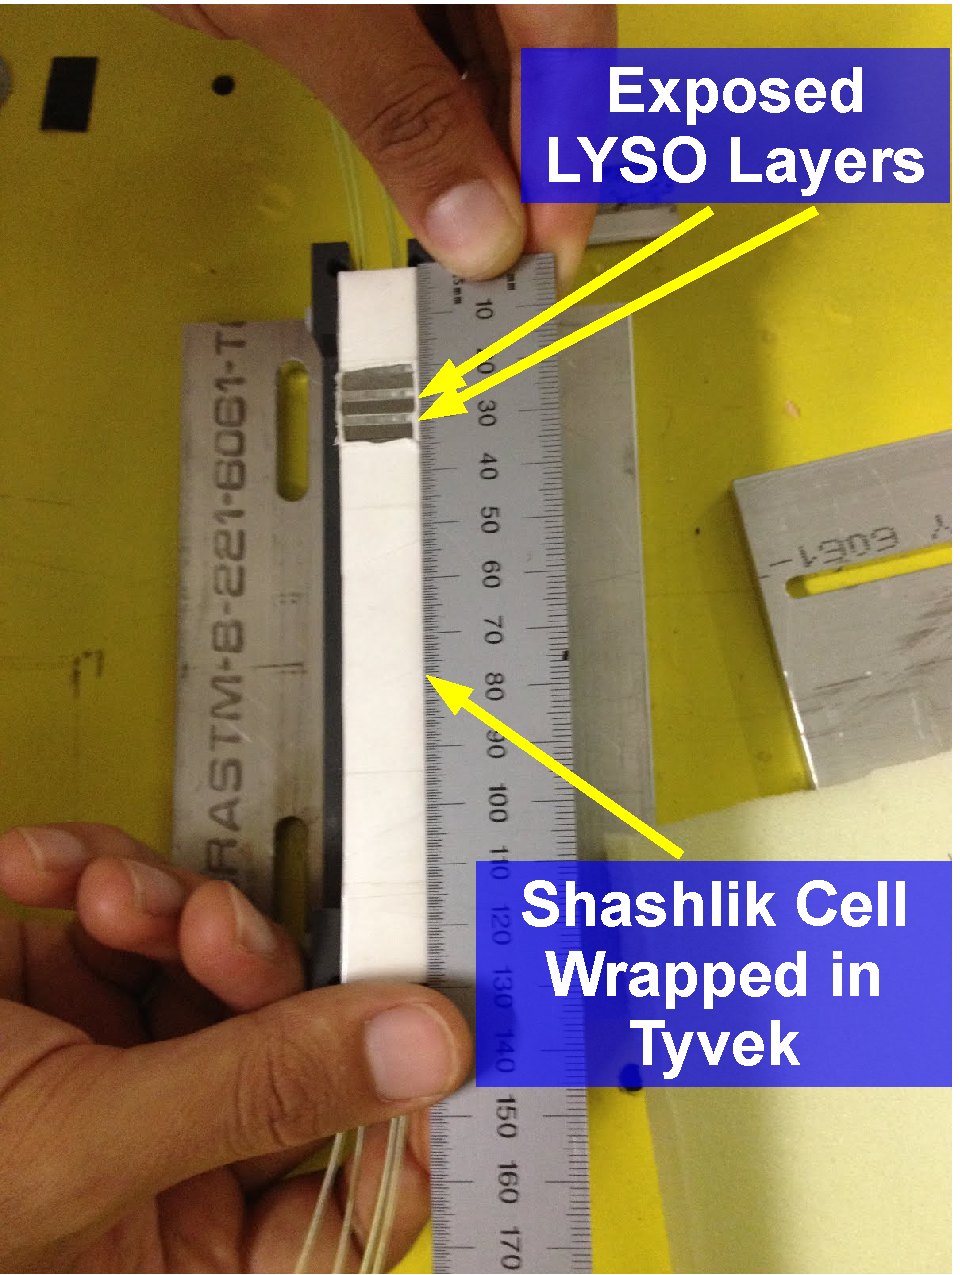
\includegraphics[width=0.30\textwidth]{figs/ShashlikSideReadoutPhotoA} 
\caption{\small A photograph of the two exposed LYSO layers in the shashlik cell.
The scintillation light signal is extracted by optically coupling
the edges of these two exposed LYSO layers to MCP-PMT
photodetectors. } 
\label{fig:ShashlikSideReadoutExposedLayersPhoto}
\end{figure}


With this setup we invoke an interplay between the light propagation jitter 
and the limited photostatistics. By placing the photodetectors in direct contact with the edges 
of two LYSO layers, we minimize the distance the scintillation light  travels to reach the 
photodetectors, and reduce the impact of light propagation jitter on the time measurement 
resolution. However in this setup we have also reduced the available photostatistics, as we collect 
light from only a small fraction of the shashlik cell. In Figure~\ref{fig:ShashlikSideReadoutTOF},
we show the time of flight distributions for electron beams at various energies,
fitted to gaussian functions. The width of the best-fit gaussian is plotted as a
function of the beam energy in Figure~\ref{fig:ShashlikSideReadoutTOFResolutionVsEnergy}. The 
best time resolution that we obtain is about $55$~ps, and fitting the result to the sum of
a $1/\sqrt{E}$ term and a constant term, we find a constant term of about
$30$~ps. 

\begin{figure}[H] \centering
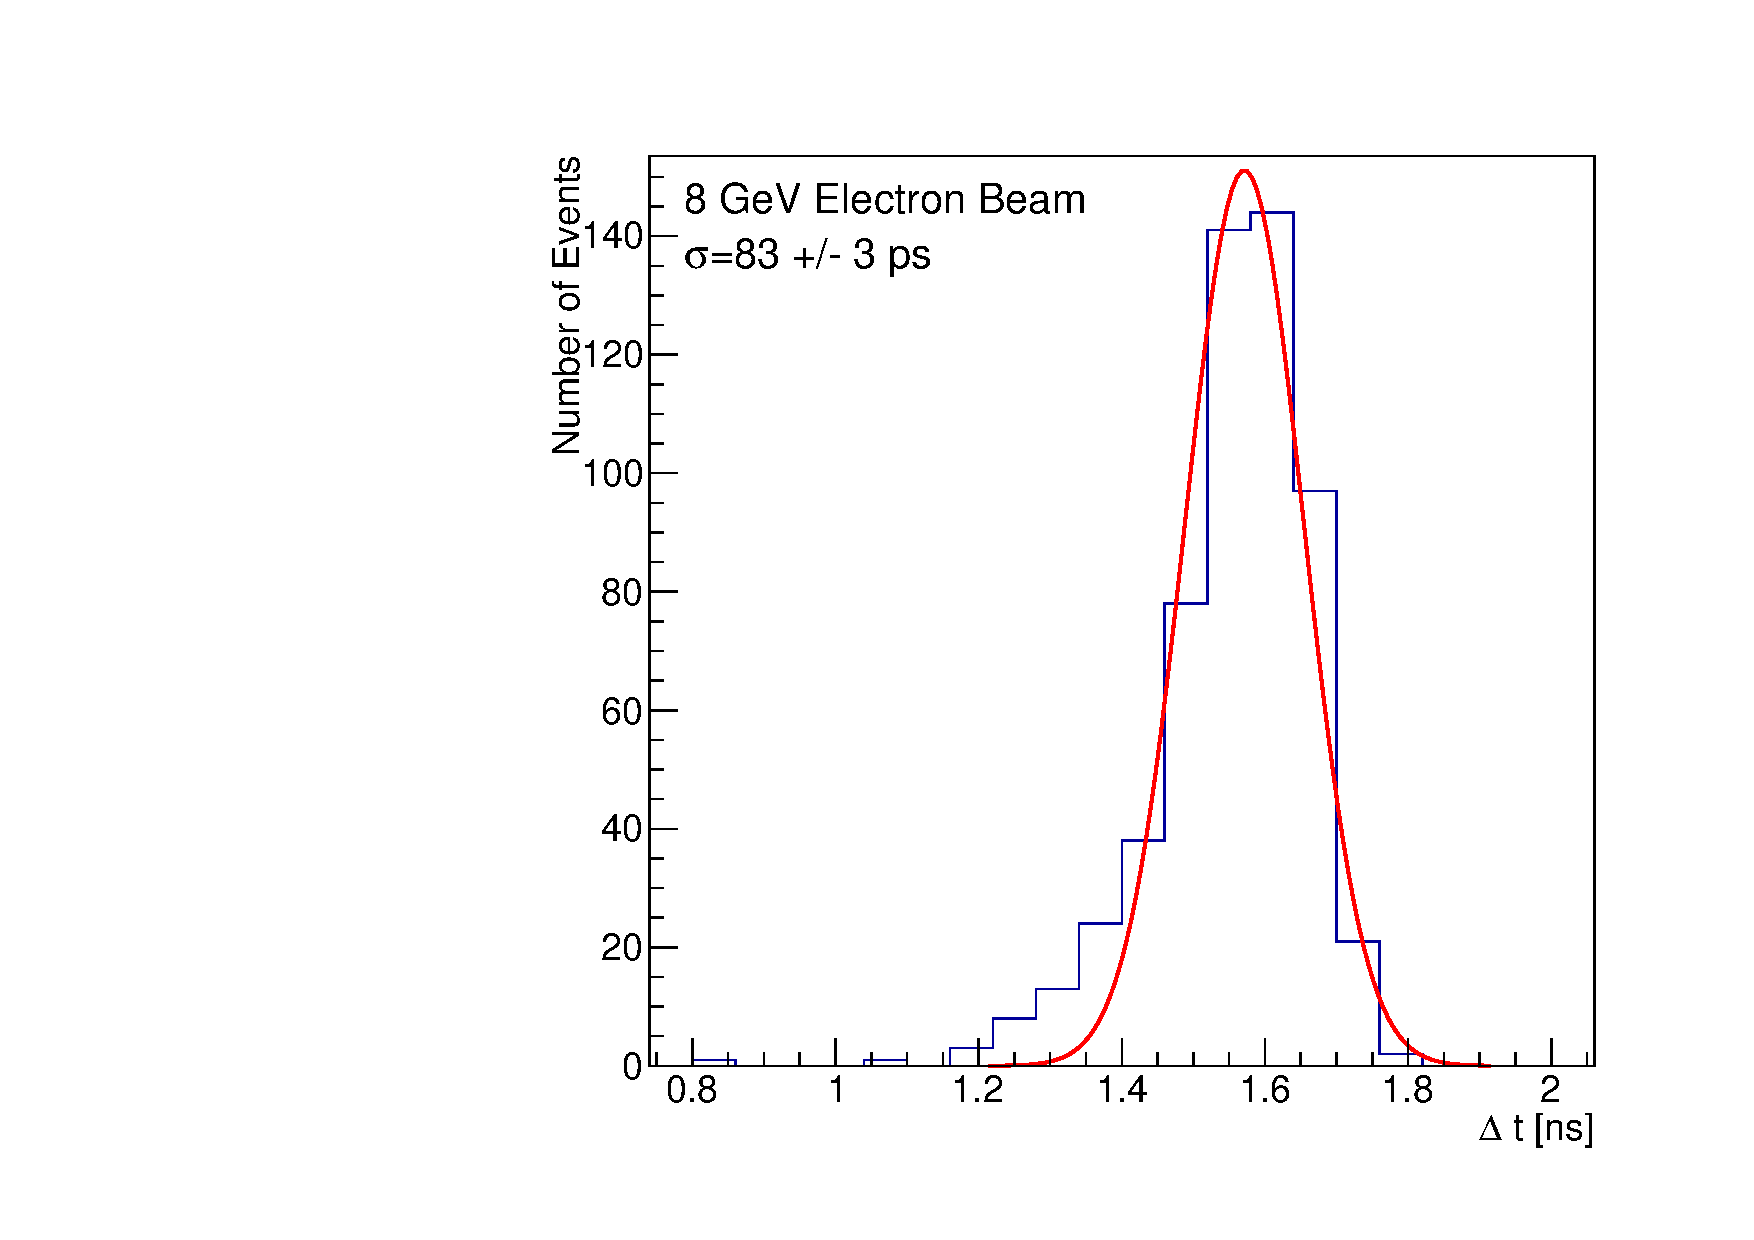
\includegraphics[width=0.32\textwidth]{figs/TOF_ShashlikSideReadout_Electron_8GeV} 
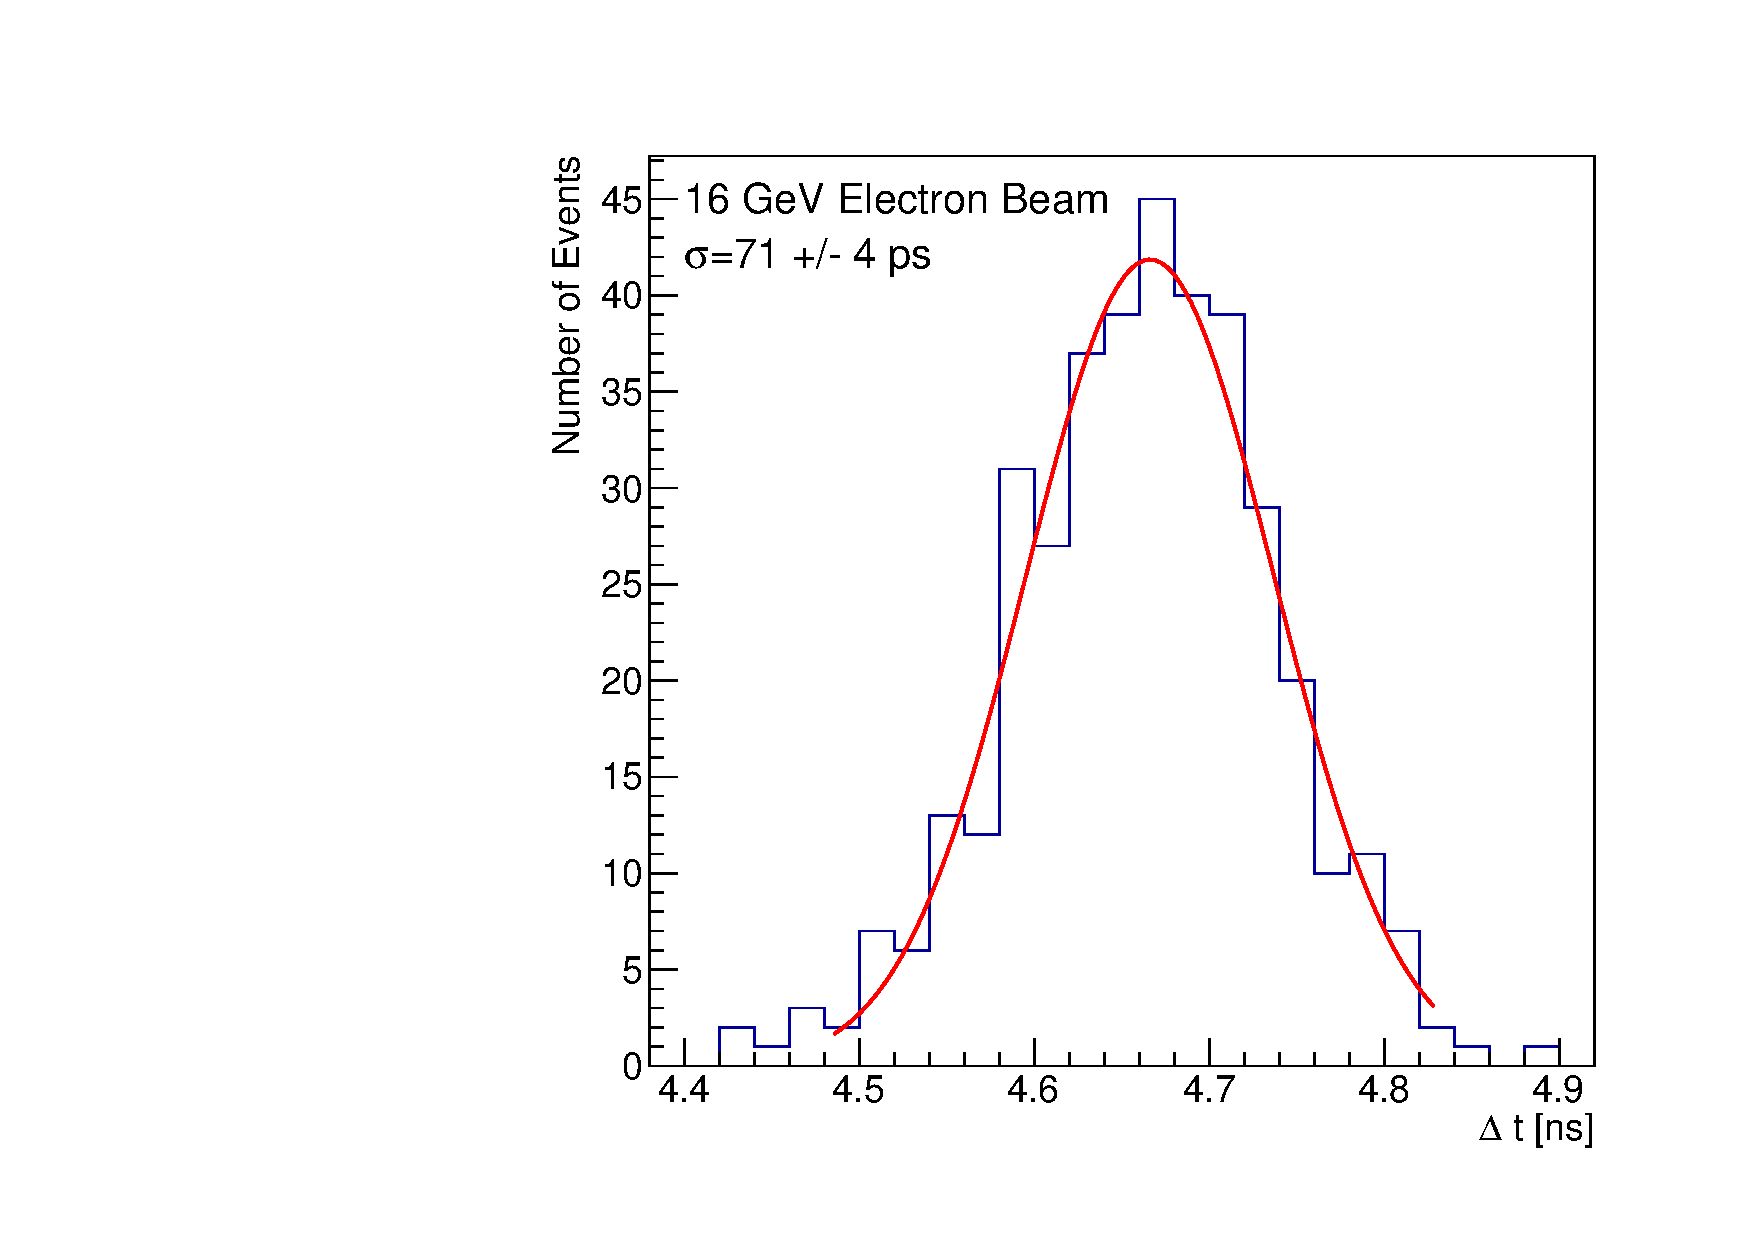
\includegraphics[width=0.32\textwidth]{figs/TOF_ShashlikSideReadout_Electron_16GeV} 
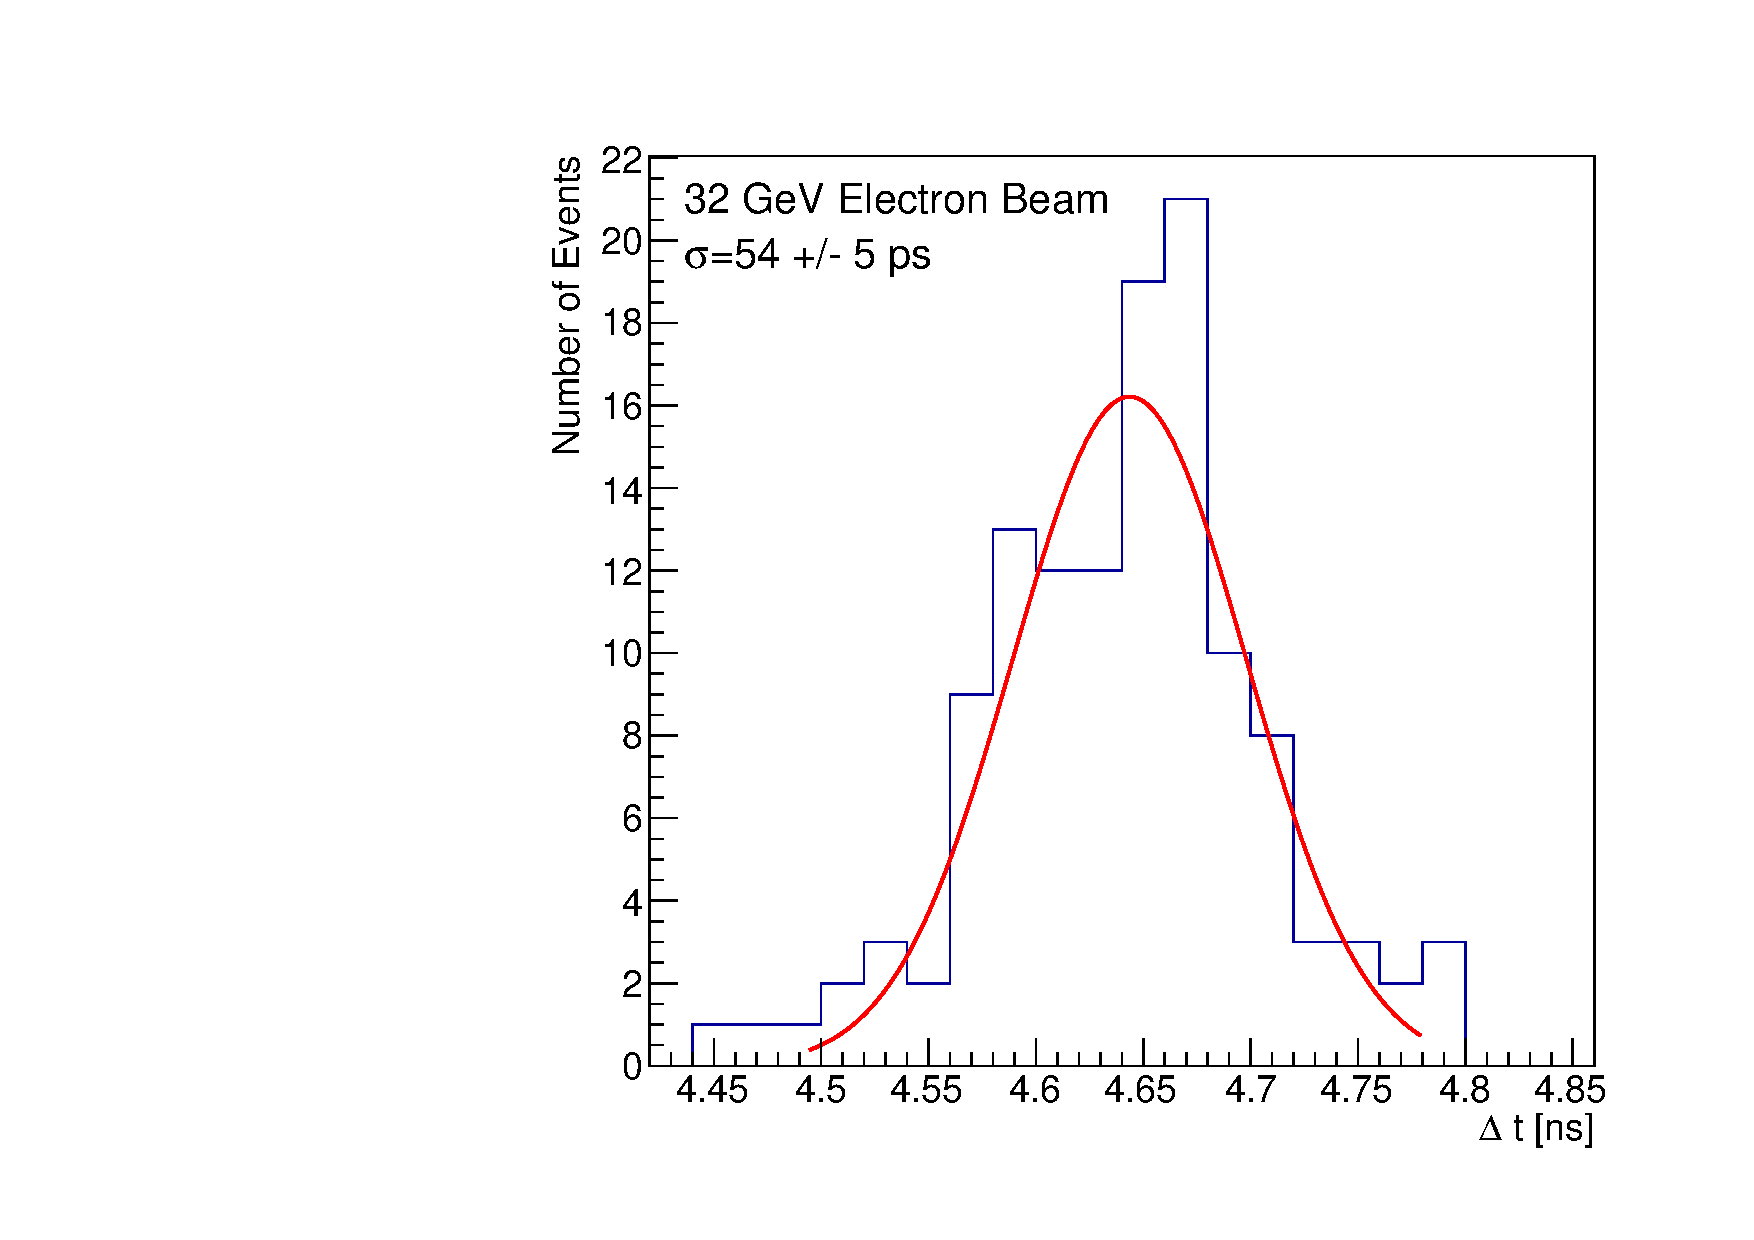
\includegraphics[width=0.32\textwidth]{figs/TOF_ShashlikSideReadout_Electron_32GeV} 
\caption{ Time of flight distributions for the LYSO-tungsten shashlik calorimeter
with signal extracted from the edges of two LYSO layers. } 
\label{fig:ShashlikSideReadoutTOF}
\end{figure}


\begin{figure}[h] \centering

\caption{\small}
\label{fig:LYSOCubeTOFResolutionVsEnergy}
\end{figure}
\begin{figure}[H] \centering
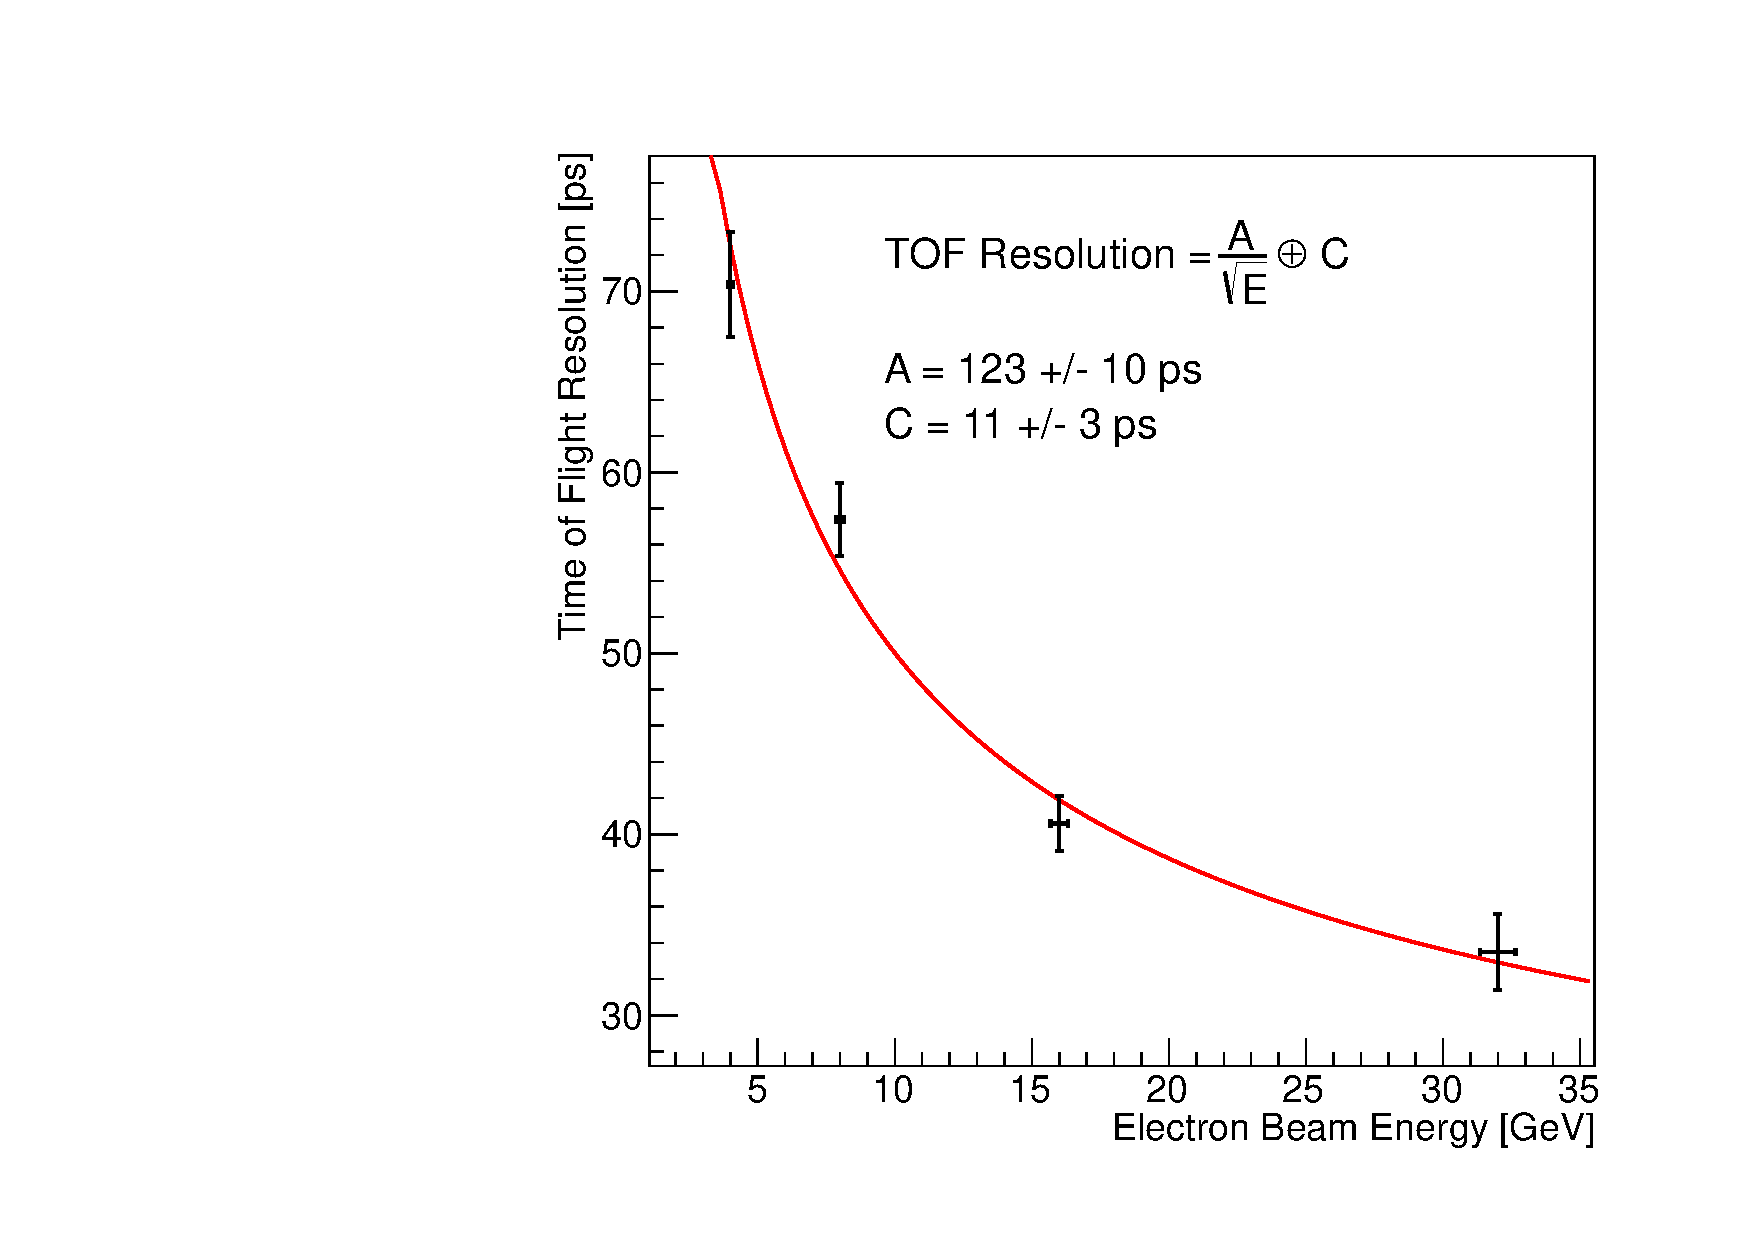
\includegraphics[width=0.32\textwidth]{figs/TimeResolutionVsEnergy_CrystalCube} 
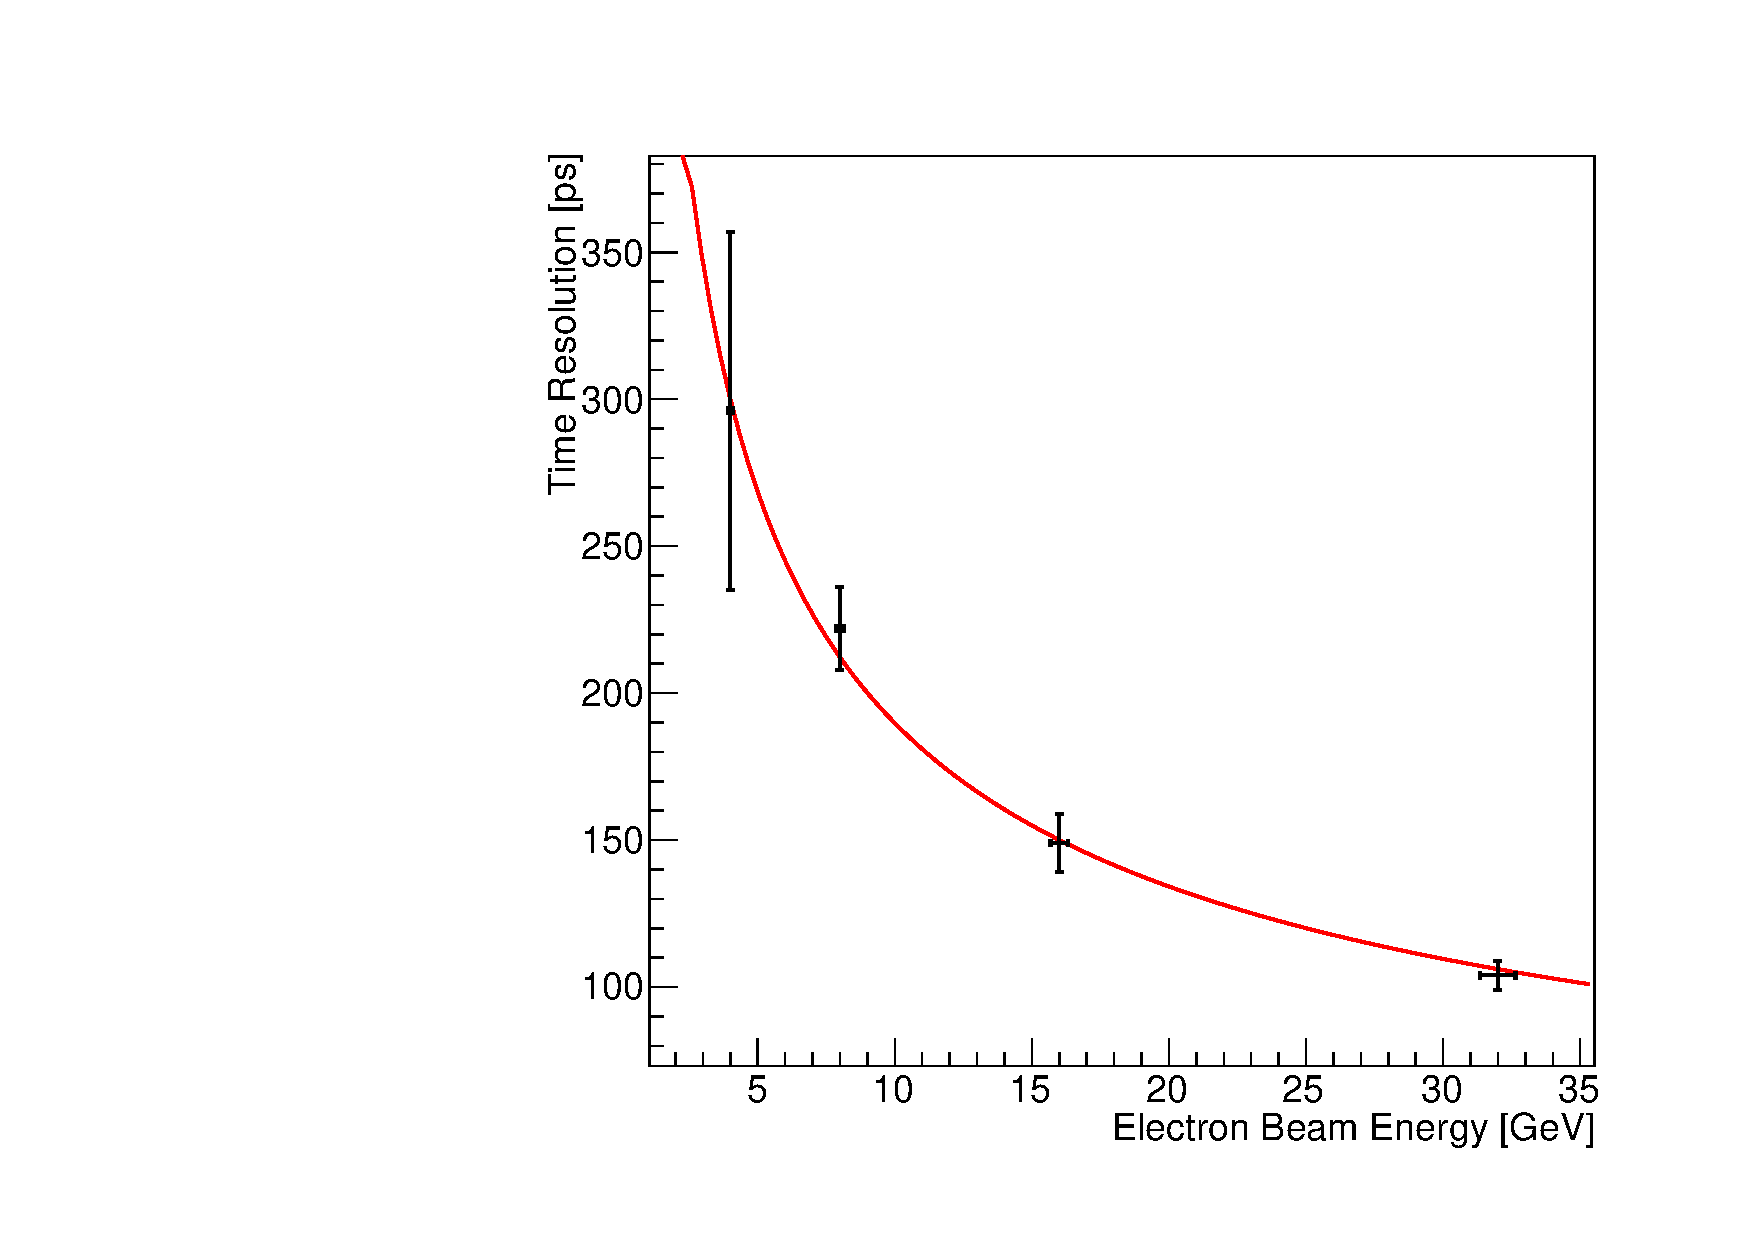
\includegraphics[width=0.32\textwidth]{figs/TimeResolutionVsEnergy_ShashlikDSB1Fiber} 
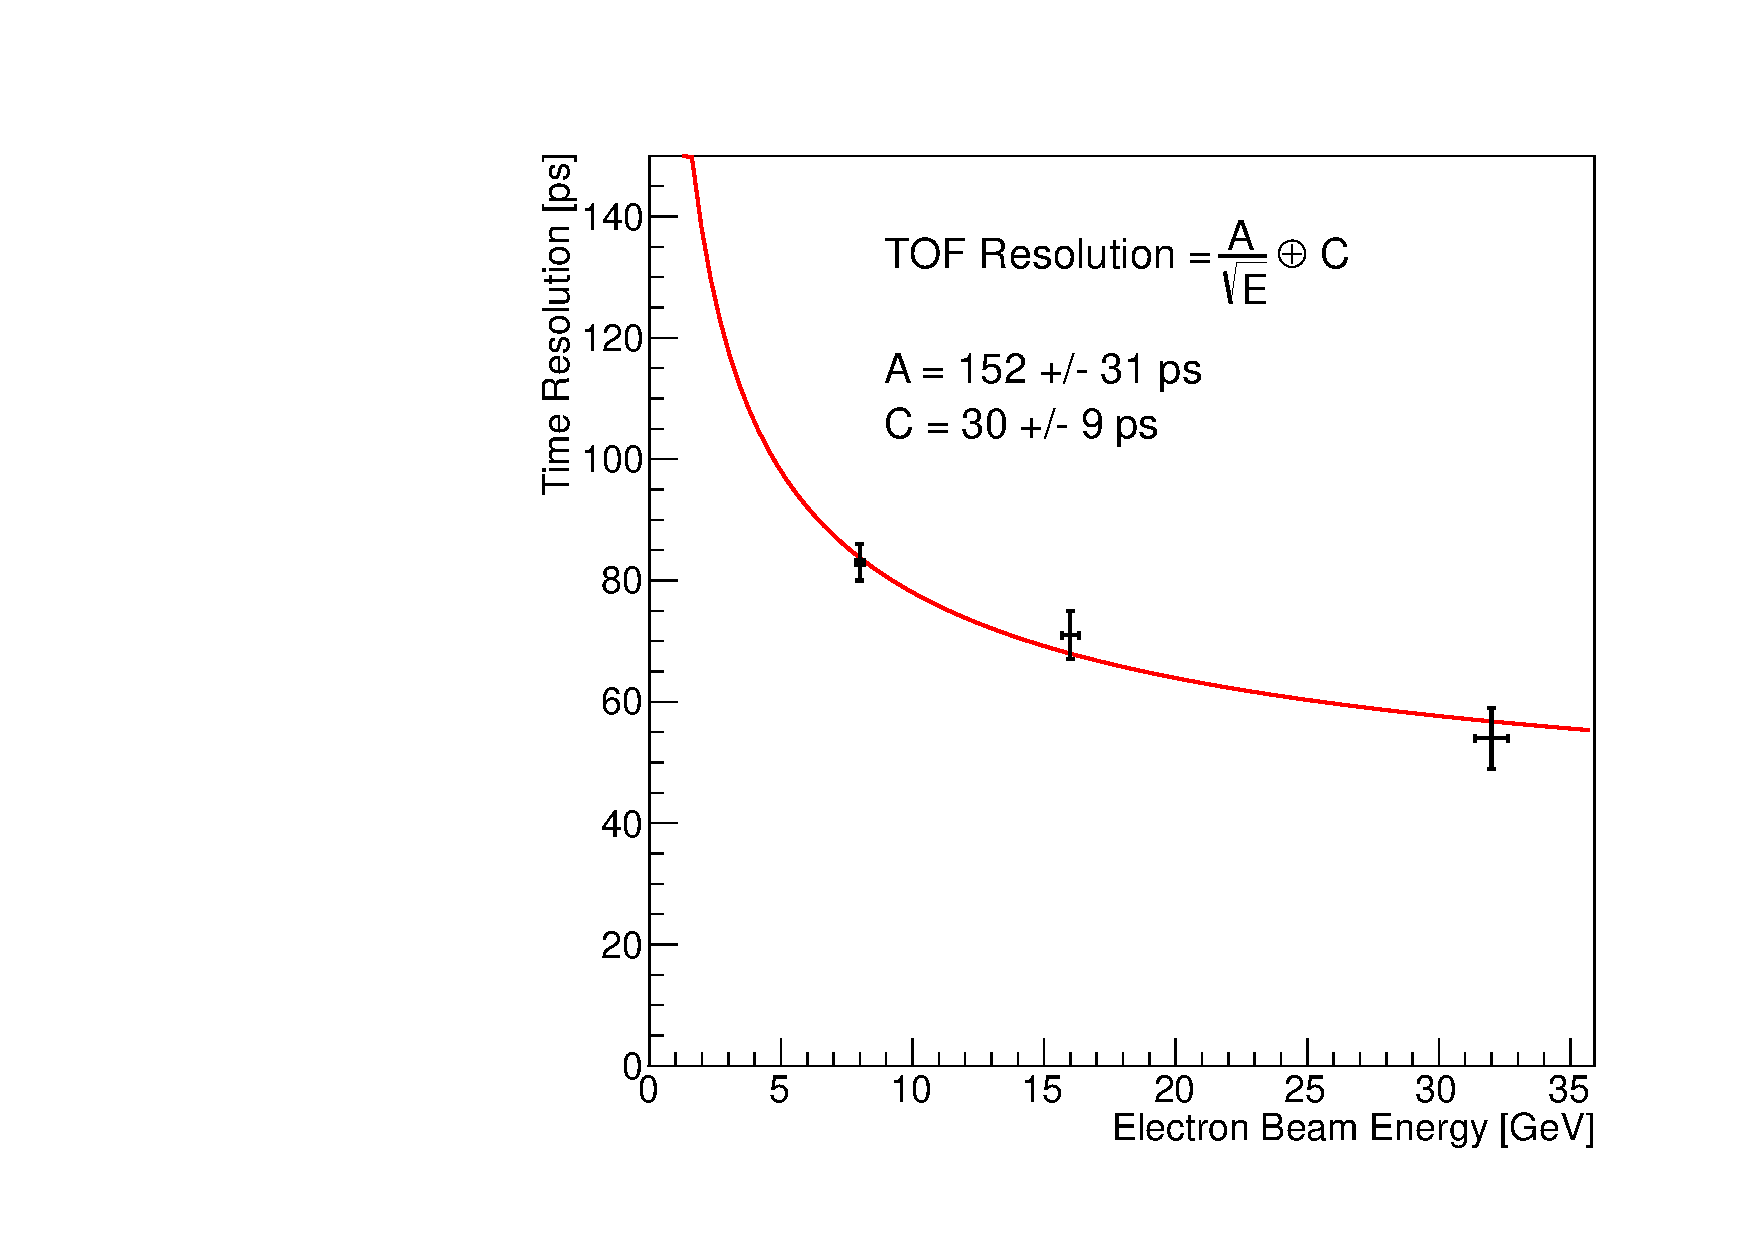
\includegraphics[width=0.32\textwidth]{figs/TimeResolutionVsEnergy_ShashlikSideReadout} 
\caption{ Timing resolution measurement as a function of the electron beam energy for (left) the LYSO cube
sampling calorimeter  
%Note that the energy absorbed in the LYSO cube is a small fraction of the incident electron energy. (Middle)The time resolution measured using  
(middle) the LYSO-tungsten shashlik
calorimeter read-out with  DSB1 fibers %is plotted as a function of
%the electron beam energy, and fitted to a $1/\sqrt{E}$ functional form. 
(right)  the LYSO-tungsten shashlik calorimeter read-out directly by optically coupling to the edges of two LYSO layers. 
%is plotted as a function of the electron beam energy, and fitted to the sum 
In all cases we fit the data with a function of $1/\sqrt{E}$  and a constant term. }
\label{fig:ShashlikSideReadoutTOFResolutionVsEnergy}
\end{figure}

In summary, we find that removing the impact of the wavelength shifting
mechanism and minimizing the impact of optical transit does indeed improve the
time resolution, but at a cost in photostatistics. Results obtained in this
experiment suggest that a LYSO-tungsten shashlik calorimeter with edge readout
can likely achieve $30$~ps resolution provided some improvement to the light
collection efficiency is achieved.

\section{Results Discussion and Summary }

In this article we have described studies characterizing the timing performance
of LYSO-based calorimeters. Using a (1.7~cm)$^{3}$ LYSO crystal that
samples the electromagnetic showers created by electrons of various energies
ranging from $4$~GeV to $32$~GeV at about $4.5$~$X_{0}$, we infer that the
contribution to the time resolution from event-by-event fluctuations of the
shower profile, the scintillation process, and the light propagation is less than
$30$~ps. Studies using different wavelength shifting fibers in a LYSO-tungsten shashlik calorimeter 
demonstrates that the choice of the fiber affects the timing performance. Besides the absorption 
and re-emission processes in the fibers, we found that another important factor influencing
the timing performance is the light extraction efficiency. Using DSB1 fibers, despite being 
photostatistics limited, we obtained a best time resolution of about $100$~ps.  A future 
development of such a detector will  be focused on increasing the light collection efficiency.
In a setup where  the scintillation light from the LYSO-tungsten
shashlik calorimeter is extracted via the edges of two LYSO layers, thereby
removing completely the wavelength shifting mechanism and long light propagation distance, 
we achieve a best time resolution of $55$~ps. The result  indicates  that such a
calorimeter design can achieve the $30$~ps time resolution benchmark achieved with the LYSO cube
provided some improvement to the light collection efficiency is achieved.

In comparing results using different light extraction schemes, we find that at a
given light yield the time resolution depends significantly on the light
propagation fluctuations. As the light yield increases the dependence on the
light propagation fluctuations is reduced. The effect can be seen in the summary
Figure~\ref{fig:ShashlikFiberAndCubeTOF} where we show the dependence of the
time resolution on the average pulse height for the shashlik cell with light
extracted through the DSB1 fibers and for the sampling calorimeter with the LYSO
cube. For the same average pulse height of 500 mV, the LYSO cube time resolution
is about half of the shashlik using the DSB1 fibers which have also twice the
rise time. As the pulse height increases the time resolution improves.
Extrapolating to the regime of very large light yield, we should be able to
reach asymptotically the best resolution without limitations from the light
propagation fluctuations. 


\begin{figure}[H] \centering
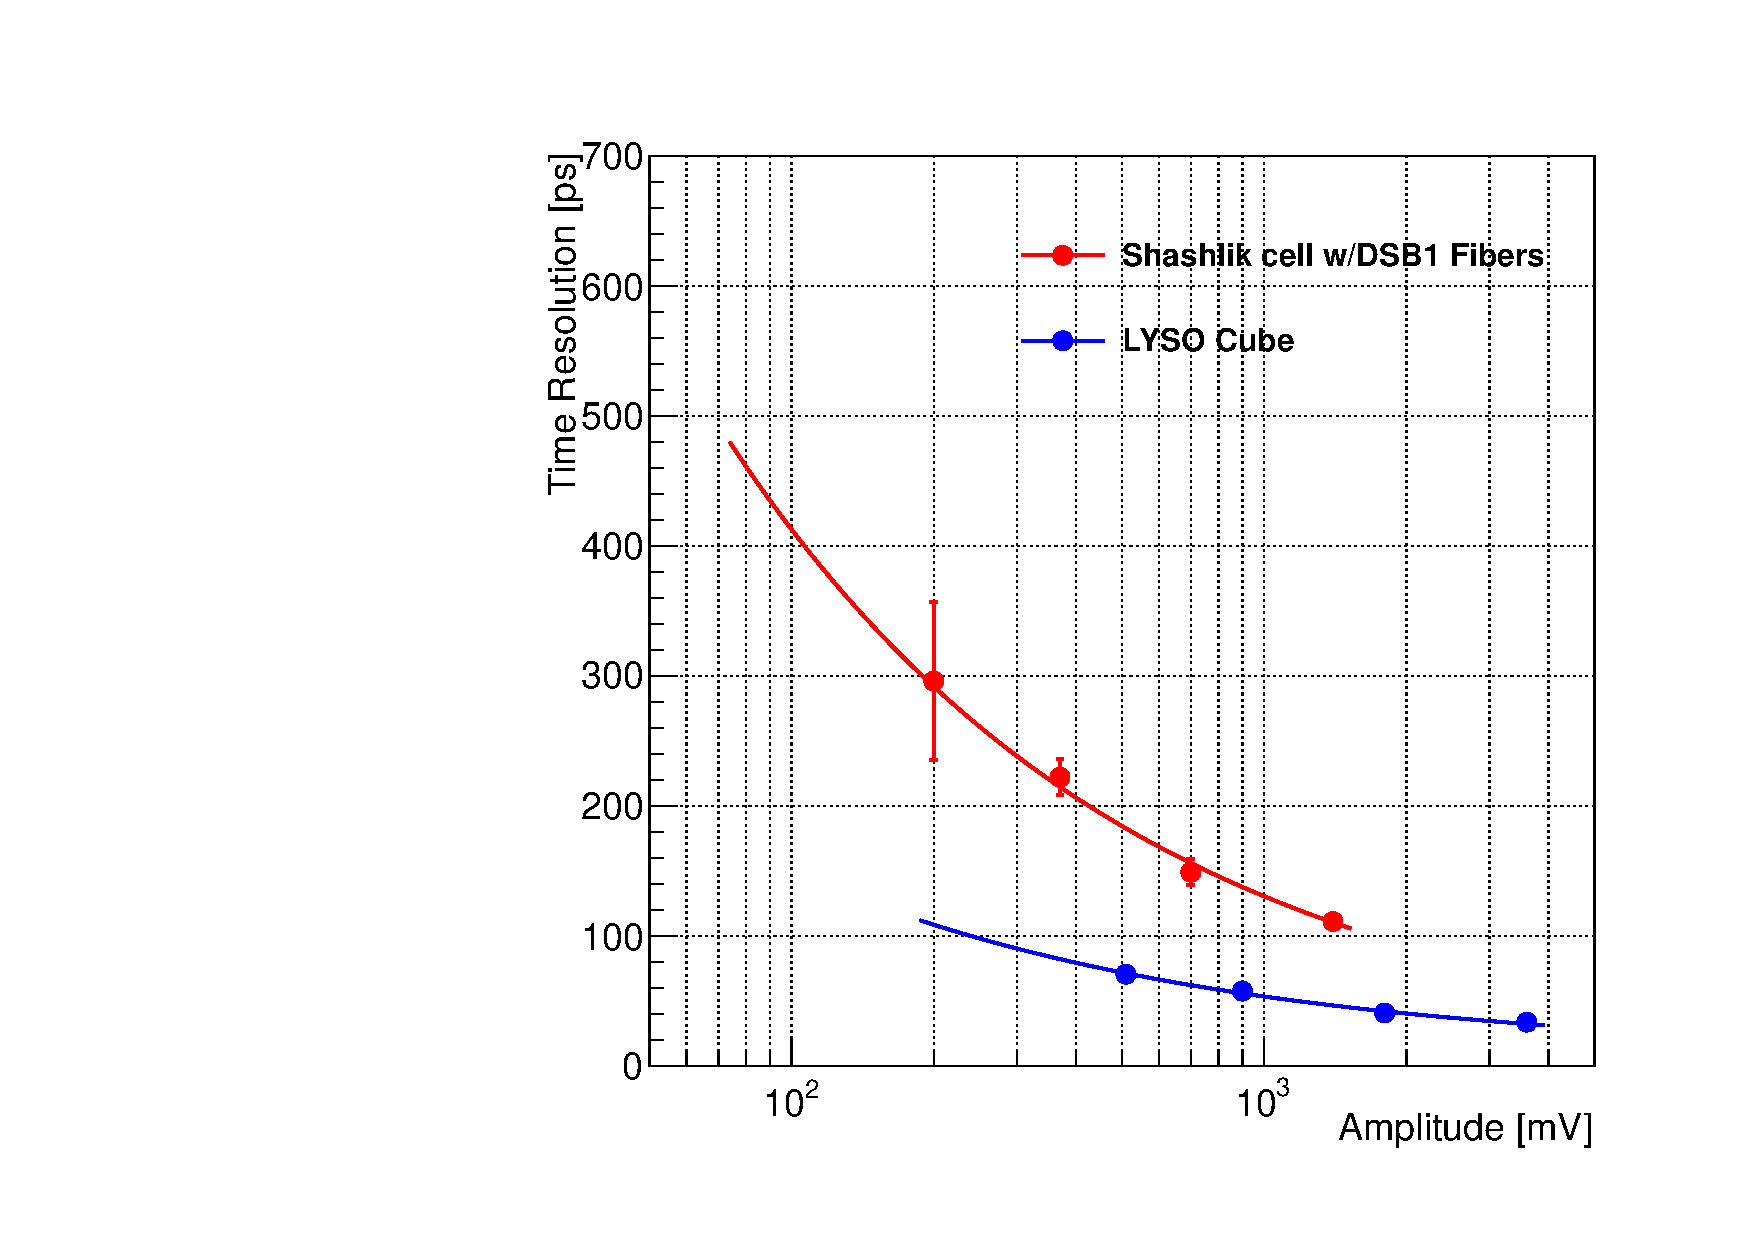
\includegraphics[width=0.55\textwidth]{figs/TimeResolutionVsEnergy_ShashlikDSB1FiberAndCube} 
\caption{\small Comparison of time resolutions obtained with the $(1.7$~cm$)^{3}$ LYSO cube (blue), 
and the LYSO-tungsten shashlik calorimeter with light extracted using DSB1 fibers (red). 
 The x-axis in this figure displays the amplitude of the
signal, corrected for the attenuation factors. }
\label{fig:ShashlikFiberAndCubeTOF}
\end{figure}

In summary, using a LYSO-based calorimeter and different light propagation experimental setups 
we obtain about $30$~ps resolution time measurement for the maximum light yield achieved. 
As a follow-up we will investigate the time resolution limitations in the limit of very large light yield, 
and attempt to improve the light collection efficiency in these types of detectors.

\section{Acknowledgements} We would like to thank Erik Ramberg and Sergey Los
for their support of our work, and Aria Soha and the FTBF test beam facility for
the good beam delivery and control. We thank Randy Ruchti for providing us with
the DSB1 fibers used in the measurements, and Eileen Hahn for the high quality
work in polishing the fibers. Thanks to Ewa Skup and Geoff Savage for help with
operation of Cherenkov counters, and to Todd Nobel for organizing and providing
supporting equipment at FTBF.


\bibliography{FastTimingPaperAug2014}{}
\bibliographystyle{ieeetr}
\end{document}    
        






























